% Chapter 1 of Bradley & Cracknell, The Mathematical Theory of Symmetry in Solids
% Rebuilt from direct page-image recognition (no MinerU). See 直接识别_ch1/工作日志.md
\documentclass[11pt,a4paper,twoside,openright]{book}
\usepackage{amsmath,amssymb}
\usepackage[margin=2.6cm]{geometry}
\usepackage{graphicx}
\usepackage{float}
\usepackage{fontspec}
\setmainfont{TeX Gyre Pagella}
\clubpenalty=10000 \widowpenalty=10000 \predisplaypenalty=10000
\setcounter{secnumdepth}{1}
\begin{document}
\chapter{Symmetry and the solid state}

\section{Introduction}

THE history of man's interest in symmetry goes back many centuries (Belov 1956\textit{b}, Coxeter and Moser 1965, Steno 1669), but its study on a modern scientific basis can be considered to have been started by the Abbé Haüy. Haüy studied the behaviour of a specimen of calcite when it was cleaved and, by breaking it into smaller and smaller pieces and studying the angles between the faces of the fragments, he convinced himself that the crystal was made up by the repetition of a large number of identical units. Haüy (1815\textit{a}–\textit{d}) studied many other crystals as well and summarized his conclusions in his so-called \textit{Loi de symétrie}. The study of symmetry developed through the nineteenth century with the formulation of ideas about point groups, Bravais lattices, and space groups.

A \textit{point group} is a set of symmetry operations acting at a point and obeying the requirements that they should form a group in the mathematical sense: the crystallographic point groups satisfy the extra requirement that they must be compatible with a space lattice. Only a finite number of different combinations of symmetry operations are observed to occur in real crystals. The derivation of these 32 point groups was published by Hessel (1830) but his work was neglected for over 30 years until they were derived again by Gadolin (1869). Since then the point groups have been studied extensively, both in their original crystallographic context and, more recently, in the context of group-theoretical studies of the physics and chemistry of molecules and solids. There are useful crystallographic texts, for example, by Buerger (1956) and Phillips (1963\textit{a}). General discussions of the theory associated with the applications of the group-theoretical studies of the point groups are given by many authors (for example; Bhagavantam and Venkatarayudu 1962, Cracknell 1968\textit{b}, Hamermesh 1962, Heine 1960, Tinkham 1964).

We can also consider another collection of groups, this time by considering translational symmetry operations. If we were to look at the internal structure of a crystal we would find that it is made up of a large number of atoms or molecules regularly arranged; it would be possible to find a set of points within the crystal which are similar. That is, the crystal looks exactly the same if viewed from any one of these points as it does if it is viewed from any other of them. If we consider such a set of identical points they make up what the mathematicians call a \textit{lattice}. It is possible to show that there is only a small number of essentially different ways of arranging a set of identical points so that the environment of each one is the same. This was done by Bravais (1850) who showed that in a three-dimensional space there are only 14 different lattices possible; consequently these are now known as \textit{Bravais lattices}, even though Frankenheim had deduced, incorrectly, 15 such lattices somewhat earlier.

A point group is concerned with the symmetry of a finite object and for natural crystals there are only 32 different point groups; a Bravais lattice is concerned with the arrangement in space of a collection of mathematical points. To study fully the internal structure of a crystal, that is, the exact detailed arrangement of the atoms within the unit cell of a crystal, one needs a further development of symmetry studies known as a \textit{space group}. A space group takes into consideration the symmetry of an arrangement of a set of identical objects, each of which is now not a point but is a finite object or a collection of atoms having some symmetry of its own. The actual operations present in a space group may be operations of the type which are present in point groups, namely pure rotations, reflections, the inversion operation, and roto-inversion or roto-reflection operations. But other operations are possible as well in a space group: they are screw rotation—and glide reflection operations—of symmetry. These are symmetry operations in which either a rotation axis or an ordinary reflection plane has a bodily movement of the crystal combined with it. In the descriptions of the derivation of the 230 space groups it is usually indicated that we owe them to Fedorov and Schönflies and sometimes the name of Barlow is added. A review of the history of the derivation of the space groups, together with a list of the publications of Barlow, Fedorov, and Schönflies, is given in an article by Burckhardt (1967). The derivation of the space groups has its origins in the works of Jordan (1868, 1869) and of Sohncke (1879). Sohncke had derived those space groups, of which there are 65, that contain only proper rotations and he noted that Jordan had previously derived them mathematically but had not translated his results into the more graphic terms of geometry. Schönflies re-derived these 65 space groups and extended the theory to include the space groups containing reflection planes of symmetry (Schönflies, 1887\textit{a}, \textit{b}, 1889, 1891). Similar results were derived by Fedorov (1885, 1891\textit{a}) but his work was written in Russian and has not become so well known in western Europe; an account of the life and work of E. S. Fedorov and a list of his publications is given (in Russian) in the book by Shafranovskiĭ (1963). It is evident that these two scientists began their works independently, one (Fedorov) as the director of a mine in the Urals and the other (Schönflies) at the suggestion of F. Klein at Göttingen, but in the course of time they heard of each other's work and compared their results. Barlow (1883) was first concerned with spherical packings and then starting with Sohncke's 65 groups he, too, obtained the remaining space groups by including reflection operations of symmetry (Barlow 1894). Burckhardt (1967) concludes that although Schönflies was not actually the first to establish the existence of the 230 space groups his writings have been the means of making their enumeration and identification generally known to the scientific world. His work, which is but little later than that of Fedorov and is quite independent, culminates in the book

\textit{Krystallsysteme und Krystallstructur} (Schönflies 1891). A letter from Schönflies to Fedorov, quoted by Burckhardt (1967), reads 'I express my great joy about the agreement with your own views; I am particularly pleased, because I am no longer alone with my theory; it will take great efforts before we shall succeed in winning over the crystallographers. \textit{I concede you the priority with pleasure}, it is of no primary importance to me.' A convenient detailed list of the space groups in modern notation can be found in Volume 1 of the \textit{International tables for X-ray crystallography} (Henry and Lonsdale 1965). At the present time there are about 9000 compounds whose space groups have been identified (for recent lists see Donnay, Donnay, Cox, Kennard, and King (1963), Nowacki, Edenharter, and Matsumoto (1967), and Wyckoff (1963, 1964, 1965, 1966, 1968)). The discovery of the two-dimensional space groups, which are also listed in detail in Volume 1 of the \textit{International tables for X-ray crystallography}, is lost in the mists of antiquity because they arose in practice, in many different civilizations, in the designs of wallpapers or tiled floors (see, for example, Coxeter and Moser (1965), p. 33).

Although studies of a vast number of crystal structures had been undertaken by X-ray methods and these crystals had been assigned to the appropriate space groups, the study of the theory of symmetry seemed not to advance very much, after the derivation of the 230 space groups in about 1890, until Shubnikov in 1951 published a book called \textit{Symmetry and anti-symmetry of finite figures} (in Russian, though this work is now translated into English, together with a list of many references to other works of Shubnikov (Shubnikov and Belov 1964)). A review of the developments in the theory of symmetry over the last 50 years is given by Koptsik (1967\textit{a}) and a brief biography of A. V. Shubnikov is given at the beginning of volume 2 of \textit{Kristallografiya} (\textit{Soviet Phys. Crystallogr.} (English transl.)) (1957)). The new developments were connected with introducing an operation of \textit{anti-symmetry}. The classical theory of symmetry, point groups, Bravais lattices, and space groups, was essentially a 3-dimensional study, that is, a point \textit{P} would be specified by the vector $\mathbf{r}\ \{=(x, y, z)\}$, and we would consider the effect of symmetry operations on this point. Shubnikov's basic idea was to say that in addition to the ordinary coordinates $x$, $y$, and $z$ of a point we now also give each point a fourth coordinate, $s$, which can only take one of two possible values. The coordinate $s$ can be the spin of a particle and the two allowed values will then correspond to spin up and spin down. Or, in purely abstract terms, they may be two colours such as black and white. If we include the coordinate $s$ and if the values of $s$ for the various atoms are randomly specified then the symmetry of the lattice has been completely destroyed. But if the spins are all parallel to a particular direction or if they are arranged in some regular fashion it is possible for some fraction of the symmetry to survive. If we introduce a new operation, which we may call the \textit{operation of anti-symmetry}, $\mathcal{R}$, and consider this in conjunction with all the ordinary point-group and space-group operations it is possible to obtain a whole collection of new point groups and space groups which are called \textit{black and white groups}, or

\textit{magnetic groups}, or \textit{Shubnikov groups}. The idea of black and white groups was actually introduced long before Shubnikov's work, by Heesch (1929\textit{a}, \textit{b}, 1930\textit{a}, \textit{b}) and also discussed by Woods (1935\textit{a}–\textit{c}), but at that time there seemed to be no very great use for these groups in the description of physical systems. It was only with the introduction of the use of neutron diffraction techniques that it became apparent that these groups could be used in the description of magnetically ordered structures. If we think of $s$ as being the two allowed values of a magnet's direction, parallel and anti-parallel to a particular direction, then $\mathcal{R}$ is the operation that reverses a magnetic moment. $\mathcal{R}$ can then be thought of as being the operation of \textit{time-inversion}.

The theory of finite groups dates from the time of Cauchy\footnote{1789–1857.} who was responsible for noticing that a number of apparently disconnected facts could be explained simultaneously by introducing the concept of a group. Galois\footnote{1811–32.} added to the theory a number of new concepts, including that of an invariant subgroup, and part of his work on the theory of equations was a first and most startling example of the power of group theory in its applications. However, it is to Serret (1866) that we owe the first connected account of group theory. Since then there has been an increasing flow of literature on the subject and today abstract group theory still flourishes as a major topic for research. Furthermore, the variety of applications of finite groups in a host of mathematical situations as diverse as the theory of permutations, the study of symmetry, and the theories of algebraic and differential equations, to mention just a few, means that a study of groups is essential for those engaged in many disciplines requiring mathematical techniques. The natural sciences are riddled with examples of problems requiring a knowledge of group theory and it is a safe assumption that the biological sciences and perhaps even the social sciences, as they become increasingly mathematical, will produce further interesting applications.

In a mathematical theory it is often possible to pick out a number of famous scholars who have been responsible for the major advances. Group theory is no exception. The only fear we have in mentioning certain names is that those of many others who have made great advances are likely to be omitted. However, it is surely no injustice to single out the names of Sylow, Frobenius, Burnside, Schur, Miller, and Mackey (apologizing immediately to Noether, Brauer, Ito, and many others who have made great contributions to the theory of abstract groups but whose work is not so directly related to the applications in this book).

Sylow (1872) made considerable progress in describing the structure of a finite group particularly in relation to its number of elements when this number is factorized as a product of primes. Frobenius (1896\textit{a}, \textit{b}, 1898) originated and was largely responsible for the theory of group representations and group characters, though Burnside (1903, 1911) made such significant simplifications and was responsible for so many original results that he also must be thought of as a group theoretician of great influence.

As a worker with a prodigious output (of approximately 800 papers between 1894 and 1946) Miller (1894, 1946) devoted considerable attention to the investigation of the structures and properties of various groups of finite order. He was responsible for determining the numbers of finite groups of various specific orders and studying the interrelationships between the structures of these groups, as exemplified by their generating relations.

The study of relations between representations of a group and those of an invariant subgroup leads inevitably to projective representations. Schur was the first to notice this and in an astounding sequence of definitive papers (1904, 1907, 1911) he not only laid the foundations of the general theory of projective representations but established most of the results that are regarded as being of particular significance. Again it was Frobenius (1898) who was responsible for the first construction of what is now called an induced representation. However, this particular notion, so important to applications in physics, was not developed significantly until after 1950 when Mackey in a series of papers (1951, 1952, 1953\textit{a}, \textit{b}, 1958) made extremely important advances that already find considerable application not only in the theory of space groups but throughout the whole realm of theoretical physics (see also Mackey (1968)).

We have described the importance of point groups, Bravais lattices, and space groups in specifying both the macroscopic symmetry of a crystal, as determined by goniometry, and the symmetry of the internal structure of a crystal, as determined by X-ray diffraction or neutron diffraction experiments. In classical physics there are some applications of group theory, such as, for instance, the investigation of the normal modes of vibration of a molecule or solid (Wigner 1930) or the determination, for a crystal belonging to a given point group, of relationships that may exist between the various components of a tensor describing some macroscopic property (see, for example, Nye (1957)). However, it was with the advent of quantum mechanics that all the powerful mathematics of group theory and representation theory really became most useful in helping to understand physical systems. Much of the pioneer work on the application of group theory in quantum mechanics was done by Weyl, Wigner, and von Neumann (see Weyl (1931), the translation of the classic book by Wigner (1959) and the collected works of von Neumann (1961, 1963)). In studying a crystal at the microscopic level one has to remember that each of the individual particles of which the crystal is composed obeys quantum mechanics rather than classical mechanics and therefore has to be described by an appropriate wave function $\psi$. The key to the application of group theory to quantum mechanics lies in the result that is expounded in Chapter 11 of Wigner's classic book (English translation, Wigner (1959)). If a quantum-mechanical system is described by the appropriate Schrödinger wave equation Wigner's theorem can be summarized as follows: '\textit{the representation of the group of the Schrödinger equation which belongs to a particular eigenvalue is uniquely determined up to a similarity transformation}.' Apart from accidental degeneracies this representation will be irreducible. The irreducible representations are therefore important because they can be used to label unambiguously the energy levels of a quantum-mechanical system. The irreducible representations of the crystallographic point groups and double point groups were determined a long time ago (Bethe 1929) and have been used extensively in labelling the energy levels of molecules (reviews and treatises include those of Eyring, Walter, and Kimball (1944), Nussbaum (1968), Rosenthal and Murphy (1936), Slater (1963), and Wilson, Decius, and Cross (1955)) in labelling the energy levels of ions or molecules in a crystal (reviews and discussions include those of Herzfeld and Meijer (1961), Hutchings (1964), Judd (1963), and McClure (1959\textit{a}, \textit{b}) and also in labelling excitons in a crystal (Overhauser 1956). A particularly useful summary of the important properties of the crystallographic point groups and their representations is given by Koster, Dimmock, Wheeler, and Statz (1963).

The theory that underlies the determination of the irreducible representations of a space group was studied by Seitz (1936\textit{b}) and first applied to symmorphic space groups by Bouckaert, Smoluchowski, and Wigner (1936), to non-symmorphic space groups by Herring (1942), and to double space groups by Elliott (1954). Subsequently, many authors have determined the irreducible representations of individual space groups and, in doing so, have employed many different sets of notation. A substantial review was written by Koster (1957) and there have recently been published some sets of complete tables of the irreducible representations of all the 230 space groups (Faddeev 1964, Kovalev 1965, Miller and Love 1967, Zak, Casher, Glück and Gur 1969). The importance of the irreducible representations of the space groups lies in the fact that, as a result of Wigner's theorem, they can be used in labelling the energy levels of a particle or quasi-particle in a crystal; they can therefore be used in labelling the electronic energy band structure and the phonon dispersion curves in crystalline solid (for reviews see Blount (1962), Jones (1960), Nussbaum (1966), Slater (1965\textit{b}, 1967) on electronic band structure, and Maradudin and Vosko (1968), Warren (1968) on phonon dispersion curves). Similarly, the irreducible representations of a space group can also be assigned to the magnon dispersion curves in a magnetic crystal. However, there is an added complication because the black and white Shubnikov space groups possess \textit{corepresentations} rather than ordinary representations (Dimmock and Wheeler 1962\textit{b}, Karavaev, Kudryavtseva, and Chaldyshev 1962, Loudon 1968, Wigner 1959, 1960\textit{a}, \textit{b}).

It is doubtful whether all the effort that workers have expended on the determination of point-group and space-group irreducible representations would be considered worth while if the only result was a scheme for labelling energy levels. However, the irreducible representations also enable one to determine the exact way in which a wave function $\psi_{i}$ will transform under the various operations of the Schrödinger group of a molecule or crystal. This often enables some simplifications to be made when an unknown wave function is expanded in terms of a set of known functions such as spherical harmonics (Altmann 1957, Altmann and Bradley 1963\textit{b}, Bell 1954, Betts 1959, McIntosh 1963, von der Lage and Bethe 1947) or plane waves (Cornwell 1969, Luehrmann 1968, Schlosser 1962, Slater 1965\textit{b}, 1967). By restricting the expansion of an unknown $\psi_{i}$ for an energy level $E_{i}$ to those functions that are known to belong to the representation of $E_{i}$ considerable simplifications can very often be achieved in the actual process of solving Schrödinger's equation to determine $\psi_{i}$. The knowledge of the transformation properties of the wave functions $\psi_{i}$ is also of importance when considering a transition of a system between two energy levels $E_{i}$ and $E_{j}$. It is then possible to use the condition that the quantum-mechanical matrix element of the transition is a pure number in order to determine, for any given perturbing potential, whether a given transition is allowed or forbidden, that is, to determine \textit{selection rules}. The group-theoretical determination of selection rules for transitions in isolated molecules and in ions or molecules in crystals involves the study of products of various point-group representations and this is discussed in the references we have already mentioned. To use the knowledge of the transformation properties of $\psi_{i}$ to study selection rules for transitions involving non-localized states in crystals is more complicated and initial work has been done by several authors (Birman 1962\textit{b}, 1963, Elliott and Loudon 1960, Lax and Hopfield 1961, Zak 1962).

\section{Group theory}

We begin the mathematical work of this book by giving a short account of the theory of groups and their representations. We do not give proofs of theorems as these appear in the first few chapters of many well-known books such as those by Hamermesh (1962), Lomont (1959), Lyubarskii (1960), and Wigner (1959). For the sake of clarity, however, we illustrate some of the definitions and theorems by means of an example; for this purpose we use a group containing six elements which, as an abstract group we call $\mathrm{G}_6^2$ (see Table 5.1) and which, in one of its realizations, is the symmetry group of an equilateral triangle.

There are two good reasons for starting with a preliminary account such as this. The first is that it makes clear what the background to the work is, and hence what it is recommended that the reader should be familiar with before proceeding with the rest of the book. The second reason is that it serves to introduce a large amount of notation; furthermore, when this is done on topics that are relatively familiar, then a reader can adjust himself more easily to the style and notation of the authors than if he is plunged immediately into new work.

The following set of definitions and theorems forms, therefore, the group-theoretical background to the work of this book. In later chapters some of them will be used as building blocks for further theorems that are either more advanced or more directly related to the study of solids. The groups that occur in the theory of solids have quite a complicated structure and, if the theorems needed for dealing with them are established rigorously and in complete detail, the proofs of such theorems require some advanced algebraic methods not commonly met in introductory courses on group theory. Some of these methods appear in Chapter 4 and they rest heavily for their appreciation on the material in this section and the next.

\textbf{DEFINITION 1.2.1.} \textit{Group.} A \textit{group} $\mathbf{G}$ is a set of elements together with a binary composition called a \textit{product} such that

\begin{quote}(i) the product of any two elements in the group is defined and is a member of the group: if $A$, $B \in \mathbf{G}$ then $AB \in \mathbf{G}$, (ii) the product is associative: $A(BC) = (AB)C$ for all $A$, $B$, $C \in \mathbf{G}$, (iii) there exists a unique identity\footnote{It is not necessary to postulate the uniqueness and two-sidedness of the identity and of the inverse elements; for the existence of a right identity ($AE = A$) and right inverses ($AA^{-1} = E$) together with axioms (i) and (ii) is sufficient to establish uniqueness and two-sidedness. However these properties are so fundamental that many authors include them in their definition.} $E$ in the group: $EA = AE = A$ for all $A \in \mathbf{G}$, and (iv) every element has a unique inverse\footnote{The group $\mathbf{H}$ is isomorphic to the subgroup $\mathbf{H}'$ of $\mathbf{G}$ consisting of elements $(H, E)$, all $H \in \mathbf{H}$. If $\mathbf{K}'$ is similarly defined then according to Definition 1.2.13 what we really have is $\mathbf{G} = \mathbf{H}' \otimes \mathbf{K}'$; however because of the isomorphism between $\mathbf{H}$ and $\mathbf{H}'$ and between $\mathbf{K}$ and $\mathbf{K}'$ it is customary to write $\mathbf{G} = \mathbf{H} \otimes \mathbf{K}$.} element: given $A \in \mathbf{G}$ there exists a unique element $A^{-1}$ such that $AA^{-1} = A^{-1}A = E$.\end{quote}

\textbf{DEFINITION 1.2.2.} \textit{Order of a group.} The number of elements in a group, $\mathbf{G}$, is called the \textit{order} of the group.

In what follows we shall be dealing only with \textit{groups of finite order}. The symbol $|\mathrm{G}|$ is often used to denote the order of $\mathbf{G}$.

\textbf{DEFINITION 1.2.3.} \textit{Order of an element.} The \textit{order of an element} $A \in \mathbf{G}$ is the least positive integer $s$ such that $A^{s} = E$.

From Definition 1.2.1 it follows that a group is completely defined by its multiplication table. In fact, it is sufficient to give a set of relations involving certain elements from which the whole multiplication table can be constructed. The elements $P_{1}$, $P_{2}$, ..., $P_{m}$ of a group $\mathbf{G}$ are called a set of \textit{generators} (or sometimes \textit{generating elements}) if every element of $\mathbf{G}$ is expressible as a finite product of powers (including negative powers) of $P_{1}$, $P_{2}$, ..., $P_{m}$. The set of relations $g_{k}(P_{1}, P_{2}, \ldots, P_{m}) = E$ ($k = 1, 2, \ldots, s$) satisfied by the generators, which are sufficient to determine the whole multiplication table of $\mathbf{G}$ are called the \textit{defining relations} (or sometimes \textit{generating relations}) of $\mathbf{G}$. For a lengthy discussion of generators and generating relations see, for example, the book by Coxeter and Moser (1965).

\textit{Example} 1.2.1. In Table 1.1 we give the multiplication table for the group $\mathbf{G}_6^2$ of order 6 whose generators are $P$ and $Q$ and whose defining relations are $P^{3} = E$, $Q^{2} = E$, and $QP = P^{2}Q$. $P$ is of order 3 and $Q$ is of order 2.

Sets of generators and defining relations are not by any means unique; in fact it is often more straightforward to take more generators than are strictly necessary. There is always, of course, a minimum number of generators without which one

cannot generate the group, but if one uses such a minimal set the defining relations can sometimes be extremely complicated and it is to avoid such complications that one often takes an over-determined set of generators. However in the simple example above we do have a minimal set.

A geometrical realization of the above group is the set of symmetry operations that carry an equilateral triangle, $\triangle ABC$, into itself. If the intersection of the medians of $\triangle ABC$ is denoted by $O$ then the operation $P$ may be thought of as the 120\textdegree  \textit{anti-clockwise} rotation about a line through $O$ perpendicular to the plane $ABC$ and $Q$ may be thought of as the reflection in the line $AO$. Equally well we could have taken $P$ to be a 120\textdegree  \textit{clockwise} rotation and $Q$ to be the reflection in $BO$, or for that matter in $CO$. In each case we would obtain the same group but with its elements labelled differently. This is a simple example of the non-uniqueness of a set of generators. In this example all six of the above sets of generators lead to the same defining relations; as we shall see in the next few paragraphs this is no accident, but on the other hand it must not be thought that different sets of generators always lead to the same defining relations.

\textbf{DEFINITION 1.2.4.} \textit{Homomorphism, isomorphism.} Given two groups $\mathbf{G}$ and $\mathbf{G}'$, a mapping $\theta$ of $\mathbf{G}$ onto $\mathbf{G}'$ which preserves multiplication is called a \textit{homomorphism}. Thus for a homomorphism $\theta$ it follows that, for all $G_{1}$, $G_{2} \in \mathbf{G}$,

\begin{equation*}
(\theta G_{1})(\theta G_{2}) = \theta(G_{1}G_{2}). \tag{1.2.1}
\end{equation*}

If in addition $\theta$ is a one-to-one mapping it is called an \textit{isomorphism}; $\mathbf{G}$ and $\mathbf{G}'$ are then said to be \textit{isomorphic}. If $\theta$ is an isomorphism and $\mathbf{G} = \mathbf{G}'$ then $\theta$ is called an \textit{automorphism}.

\textit{Example} 1.2.2. Let $\mathbf{G} = \mathbf{G}_6^2$ and $\mathbf{G}' = \mathbf{G}_2^1$, the cyclic group of order 2 composed of elements $E$ and $P'$ with $P'^{2} = E$ ($E$ being the identity) (see Table 5.1). Then if $\theta$ is defined so that $\theta E = E$, $\theta P = E$, $\theta P^{2} = E$, $\theta Q = P'$, $\theta(PQ) = P'$, and $\theta(P^{2}Q) = P'$, then $\theta$ is a homomorphism of $\mathbf{G}_6^2$ onto $\mathbf{G}_2^1$.

\bigskip\hrule\bigskip

\begin{minipage}{\textwidth}
\centering\textbf{TABLE 1.1}
\textit{The multiplication table for the group} $\mathbf{G}_6^2$.

\centering
\begin{tabular}{|l|l|l|l|l|l|}
\hline
 & $P$ & $P^{2}$ & $Q$ & $PQ$ & $P^{2}Q$ \\ \hline
$E$ & $P$ & $P^{2}$ & $Q$ & $PQ$ & $P^{2}Q$ \\ \hline
$P$ & $P^{2}$ & $E$ & $PQ$ & $P^{2}Q$ & $Q$ \\ \hline
$P^{2}$ & $E$ & $P$ & $P^{2}Q$ & $Q$ & $PQ$ \\ \hline
$Q$ & $P^{2}Q$ & $PQ$ & $E$ & $P^{2}$ & $P$ \\ \hline
$PQ$ & $Q$ & $P^{2}Q$ & $P$ & $E$ & $P^{2}$ \\ \hline
$P^{2}Q$ & $PQ$ & $Q$ & $P^{2}$ & $P$ & $E$ \\ \hline
\end{tabular}
\end{minipage}
\medskip

\textit{Notes to Table 1.1.}

\begin{quote}(i) The generating relations of this group are: $P^{3} = E$; $Q^{2} = E$; $QP = P^{2}Q$. (ii) In order to obtain a product $LM$ take the element in the row beginning with $L$ and the column headed $M$. Thus, for example, $(PQ)(P^{2}Q) = P^{2}$.\end{quote}

On the other hand, if it is given that $\theta$ is a homomorphism of $\mathbf{G}_6^2$ onto $\mathbf{G}_2^1$ then, by virtue of eqn. (1.2.1), it is sufficient in order to define $\theta$ to specify its action only on the generators of $\mathbf{G}_6^2$. Thus, if $\theta$ is a homomorphism, $\theta P = E$ and $\theta Q = P'$ defines $\theta$ completely.

\textit{Example} 1.2.3. Let $\mathbf{G} = \mathbf{G}' = \mathbf{G}_6^2$. Then if $\phi$ is such that $\phi(E) = E$, $\phi(P) = P^{2}$, $\phi(P^{2}) = P$, $\phi(Q) = Q$, $\phi(PQ) = P^{2}Q$, and $\phi(P^{2}Q) = PQ$, $\phi$ is an automorphism of $\mathbf{G}_6^2$ onto itself.

\textbf{THEOREM 1.2.1.} \textit{If $\phi_{1}$ and $\phi_{2}$ are two automorphisms of a group $\mathbf{G}$ then the mapping product $\phi_{1}\phi_{2}$ (where $(\phi_{1}\phi_{2})G = \phi_{1}(\phi_{2}G)$ for all $G \in \mathbf{G}$) is also an automorphism. Further the set of all automorphisms of a group $\mathbf{G}$ is itself a group $\mathbf{A}(\mathbf{G})$ of which the binary composition is the mapping product just defined.}

\textit{Example} 1.2.4. Consider $\mathbf{A}(\mathbf{G}_6^2)$. It is a group of six elements. Its generators may be taken to be $\phi$, as defined in Example 1.2.3, and $\rho$, where $\rho(P) = P$ and $\rho(Q) = P^{2}Q$. If the identity automorphism is denoted by $\varepsilon$ then $\phi^{2} = \varepsilon$, $\rho^{3} = \varepsilon$, and $\phi\rho = \rho^{2}\phi$. Let $\mathbf{G} = \mathbf{G}_6^2$ and $\mathbf{G}' = \mathbf{A}(\mathbf{G}_6^2)$. Then $\mathbf{G}$ and $\mathbf{G}'$ are isomorphic under the mapping $\alpha$: $\alpha P = \rho$ and $\alpha Q = \phi$.

\textit{Example} 1.2.5. $\mathbf{G}_6^2$ is isomorphic with $\mathbf{S}_3$, the group of permutations of three identical objects.

\textit{Example} 1.2.6. Example 1.2.4 explains the six possible sets of generators for $\mathbf{G}_6^2$ mentioned at the end of Example 1.2.1, for each automorphism leads to a different labelling of the group.

\textbf{DEFINITION 1.2.5.} \textit{Kernel.} If $\theta\mathbf{G} = \mathbf{G}'$ is a homomorphism of $\mathbf{G}$ onto $\mathbf{G}'$ then the \textit{kernel} of $\theta$ is the set of elements of $\mathbf{G}$ that is mapped onto the identity of $\mathbf{G}'$.

\textit{Example} 1.2.7. The kernel of an isomorphism consists of one element only, the identity of $\mathbf{G}$.

\textit{Example} 1.2.8. The kernel of the homomorphism $\theta$ defined in Example 1.2.2 consists of the elements $E$, $P$, and $P^{2}$.

\textbf{DEFINITION 1.2.6.} \textit{Subgroup.} A subset $\mathbf{H}$ of a group $\mathbf{G}$ that is itself a group under the same binary composition as in $\mathbf{G}$ is called a \textit{subgroup} of $\mathbf{G}$.

\textit{Example} 1.2.9. The following are subgroups of $\mathbf{G}_6^2$: (i) $\mathbf{G}_6^2$ itself, (ii) $\mathbf{G}_3^1$, consisting of $E$, $P$, and $P^{2}$, (iii) $\mathbf{G}_2^1$, consisting of $E$ and $Q$, (iv) $\mathbf{G}_2^{1'}$, consisting of $E$ and $PQ$, (v) $\mathbf{G}_2^{1''}$, consisting of $E$ and $P^{2}Q$, and (vi) $\mathbf{G}_1^1$, consisting of the identity $E$ alone.

A group always has at least two subgroups, namely the group itself and the group consisting of the identity alone. Such subgroups are called \textit{improper subgroups}. Other subgroups besides these two are called \textit{proper subgroups}. Thus $\mathbf{G}_6^2$ has 4 proper subgroups.

If $\mathbf{H}$ is a subset of $\mathbf{G}$ consisting of $t$ elements ($H_{1}$, $H_{2}$, ..., $H_{t}$) then by $\mathbf{AH}$, $A \in \mathbf{G}$, we mean the subset of $t$ elements ($AH_{1}$, $AH_{2}$, ..., $AH_{t}$).

If $\mathbf{K}$ is a subset of $\mathbf{G}$ consisting of $s$ elements ($K_{1}$, $K_{2}$, ..., $K_{s}$) then by $\mathbf{KH}$ we mean the set of $st$ elements $K_{i}H_{j}$ ($i = 1$ to $s$, $j = 1$ to $t$); by $\mathbf{H} + \mathbf{K}$ we mean the set of $(t+s)$ elements ($H_{1}$, $H_{2}$, ..., $H_{t}$, $K_{1}$, $K_{2}$, ..., $K_{s}$).

\textbf{DEFINITION 1.2.7.} \textit{Conjugate elements.} Two elements $G_{1}$, $G_{2} \in \mathbf{G}$ are said to be \textit{conjugate} if there exists an element $G \in \mathbf{G}$ such that $G_{2} = GG_{1}G^{-1}$.

\textit{Example} 1.2.10. In the group $\mathbf{G}_6^2$, $P$ and $P^{2}$ form a pair of conjugate elements. For it follows immediately from the defining relations that $P^{2} = QPQ^{-1}$ and $P = QP^{2}Q^{-1}$.

\textbf{DEFINITION 1.2.8.} \textit{Abelian group.} If $\mathbf{G}$ is a group and $G_{1}G_{2} = G_{2}G_{1}$ for all $G_{1}$, $G_{2} \in \mathbf{G}$ then $\mathbf{G}$ is called an \textit{Abelian group} (or sometimes a \textit{commutative group}).

\textit{Example} 1.2.11. The group $\mathbf{G}_3^1$ mentioned in Example 1.2.9 is an Abelian group.

\textbf{THEOREM 1.2.2.} \textit{A group} $\mathbf{G}$ \textit{splits into 'conjugacy classes' $C_{1}$, $C_{2}$, ..., $C_{r}$ such that the following properties hold:}

\begin{quote}(i) \textit{every element of} $\mathbf{G}$ \textit{is in some class, and no element of} $\mathbf{G}$ \textit{is in more than one class, so that} $\mathbf{G} = C_{1} + C_{2} + \ldots + C_{r}$, (ii) \textit{all the elements in a given class are mutually conjugate and consequently have the same order (though, of course, not all elements of the same order necessarily belong to the same class),} (iii) \textit{an element that commutes with all elements of the group is in a class by itself and is called a 'self-conjugate' element (the identity is always in a class by itself, and, further, if} $\mathbf{G}$ \textit{is Abelian then every element of} $\mathbf{G}$ \textit{is in a class by itself),} (iv) \textit{the number of elements in a class is a divisor of the order of the group,} (v)

\begin{equation*}
C_{i}C_{j} = \sum_{k=1}^{r} h_{ij,k}C_{k} \tag{1.2.2}
\end{equation*}

\textit{where the coefficients $h_{ij,k}$ are called the 'class multiplication coefficients' and are positive integers or zero. Also}

\begin{equation*}
h_{ij,k} = h_{ji,k}. \tag{1.2.3}
\end{equation*}
\end{quote}

\textit{Example} 1.2.12. For the group $\mathbf{G}_6^2$ take $C_{1} = E$; $C_{2} = P$, $P^{2}$; and $C_{3} = Q$, $PQ$, $P^{2}Q$. Then the conditions of Theorem 1.2.2 are satisfied with $r = 3$. Elements in $C_{2}$ are of order 3, and elements in $C_{3}$ are of order 2. The identity is the only element to be in a class by itself. 1, 2, and 3, the numbers of elements in the classes $C_{1}$, $C_{2}$, and $C_{3}$ are divisors of 6, the order of $\mathbf{G}_6^2$. The values of the $h_{ij,k}$ can easily be evaluated by using Table 1.1. They are $h_{11,1} = 1$, $h_{12,2} = 1$, $h_{13,3} = 1$, $h_{22,1} = 2$, $h_{22,2} = 1$, $h_{23,3} = 2$, $h_{33,1} = 3$, $h_{33,2} = 3$, and all others not derived from these by eqn. (1.2.3) are zero.

\textbf{DEFINITION 1.2.9.} \textit{Coset.} If $\mathbf{H}$ is a subgroup of $\mathbf{G}$ and $A$ is any element of $\mathbf{G}$ then the subset $\mathbf{H}A$ is called a \textit{right coset} of $\mathbf{H}$; similarly $A\mathbf{H}$ is called a \textit{left coset}. $A$ is called the \textit{coset representative} (and is not in any way special because if $B \in \mathbf{H}A$ then the coset $\mathbf{H}B = \mathbf{H}A$, so that any element of a coset can serve as the coset representative).

\textbf{THEOREM 1.2.3.} \textit{A group} $\mathbf{G}$ \textit{with a subgroup} $\mathbf{H}$ \textit{splits up into 'left cosets' of} $\mathbf{H}$. \textit{The following properties hold:}

\begin{quote}(i) \textit{every element of} $\mathbf{G}$ \textit{is in some left coset and no element of} $\mathbf{G}$ \textit{is in more than one left coset,} (ii) \textit{every left coset contains the same number of elements, this number being equal to the order of} $\mathbf{H}$. \textit{Thus the order of} $\mathbf{H}$ \textit{is a divisor of the order of} $\mathbf{G}$; \textit{the quotient} $|\mathbf{G}|/|\mathbf{H}|$, \textit{which is just the number, $t$, of left cosets of} $\mathbf{H}$, \textit{is called the 'index' of} $\mathbf{H}$ \textit{in} $\mathbf{G}$.\end{quote}

\textit{Example} 1.2.13. Take $\mathbf{G} = \mathbf{G}_6^2$ and $\mathbf{H} = \mathbf{G}_3^1$, consisting of $E$, $P$, and $P^{2}$. If we write $\mathbf{G}_6^2 = (E\mathbf{G}_3^1 + Q\mathbf{G}_3^1)$ then this is a decomposition of $\mathbf{G}_6^2$ satisfying the conditions of Theorem 1.2.3 with $t = 2$.

\textit{Example} 1.2.14. From Example 1.2.9 the orders of the subgroups of $\mathbf{G}_6^2$ are seen to be 1, 2, 3, and 6, and these numbers are all divisors of 6, the order of $\mathbf{G}_6^2$. This division property is called Lagrange's theorem.

\textbf{DEFINITION 1.2.10.} \textit{Invariant subgroup.} If $\mathbf{H}$ is a subgroup of $\mathbf{G}$ such that, for all $G \in \mathbf{G}$ and all $H \in \mathbf{H}$, $GHG^{-1} \in \mathbf{H}$, then $\mathbf{H}$ is said to be an \textit{invariant subgroup} (or sometimes a \textit{normal subgroup} or a \textit{self-conjugate subgroup}) of $\mathbf{G}$.

\textbf{THEOREM 1.2.4.} \textit{If} $\mathbf{H}$ \textit{is a subgroup of} $\mathbf{G}$ \textit{then} $\mathbf{H}$ \textit{is invariant if and only if} $A\mathbf{H} = \mathbf{H}A$ \textit{for all} $A \in \mathbf{G}$; \textit{that is, if and only if all right and left cosets coincide.}

\textit{Example} 1.2.15. An immediate result from Theorem 1.2.4 is that all subgroups of index 2 are invariant subgroups. In particular, we see from Example 1.2.13 that $\mathbf{G}_3^1$ is invariant in $\mathbf{G}_6^2$.

\textbf{DEFINITION 1.2.11.} \textit{Inner automorphism.} The mapping $\beta$ from $\mathbf{G}$ onto itself such that $\beta G = BGB^{-1}$ for all $G \in \mathbf{G}$ (and where $B$ is a fixed element of $\mathbf{G}$) is an automorphism, and an automorphism produced by conjugation in this way is called an \textit{inner automorphism} (all others being called \textit{outer automorphisms}).

\textit{Example} 1.2.16. All automorphisms of $\mathbf{G}_6^2$ are inner. Indeed it can soon be verified from Example 1.2.4 and Table 1.1 that $\rho$ corresponds to conjugation by $P$ and $\phi$ corresponds to conjugation by $Q$.

\textbf{THEOREM 1.2.5.} \textit{A subgroup} $\mathbf{H}$ \textit{of} $\mathbf{G}$ \textit{is an invariant subgroup if and only if} $\mathbf{H}$ \textit{is invariant under all inner automorphisms of} $\mathbf{G}$.

\textbf{THEOREM 1.2.6.} \textit{A subgroup} $\mathbf{H}$ \textit{of} $\mathbf{G}$ \textit{is invariant if and only if} $\mathbf{H}$ \textit{is composed of entire conjugacy classes of} $\mathbf{G}$.

\textit{Example} 1.2.17. From Theorem 1.2.6 and Examples 1.2.9 and 1.2.13 it follows at once that the subgroup $\mathbf{G}_3^1$ is the only proper invariant subgroup of $\mathbf{G}_6^2$.

\textbf{DEFINITION 1.2.12.} \textit{Simple groups.} If a group $\mathbf{G}$ has no proper invariant subgroup then it is said to be \textit{simple}. If a group $\mathbf{G}$ has no proper invariant Abelian subgroup it is said to be \textit{semi-simple}.

\textit{Example} 1.2.18. $\mathbf{G}_6^2$ is not simple. Nor is it even semi-simple, for its subgroup $\mathbf{G}_3^1$ is a proper invariant Abelian subgroup.

\textbf{THEOREM 1.2.7.}

\begin{quote}(i) \textit{If} $\mathbf{H}$ \textit{is an invariant subgroup of} $\mathbf{G}$ \textit{then the left cosets of} $\mathbf{H}$ \textit{form a group with binary composition defined by the equation}

\begin{equation*}
(G_{i}\mathbf{H})(G_{j}\mathbf{H}) = (G_{i}G_{j})\mathbf{H}. \tag{1.2.4}
\end{equation*}

\textit{This group is called the quotient group} $\mathbf{G}/\mathbf{H}$ \textit{and its order is equal to the index of} $\mathbf{H}$ \textit{in} $\mathbf{G}$. \textit{The identity of} $\mathbf{G}/\mathbf{H}$ \textit{is the subgroup} $\mathbf{H}$ \textit{itself.}

(ii) \textit{If $\theta$ is a homomorphism of} $\mathbf{G}$ \textit{onto} $\mathbf{G}'$ \textit{and} $\mathbf{H}$ \textit{is the kernel of $\theta$ then} $\mathbf{H}$ \textit{is an invariant subgroup of} $\mathbf{G}$ \textit{and} $\mathbf{G}'$ \textit{is isomorphic to} $\mathbf{G}/\mathbf{H}$.

(iii) \textit{Conversely, if} $\mathbf{H}$ \textit{is an invariant subgroup of} $\mathbf{G}$ \textit{and $\theta$ is a mapping of} $\mathbf{G}$ \textit{onto} $\mathbf{G}/\mathbf{H}$ \textit{such that $\theta G = G\mathbf{H}$ for all} $G \in \mathbf{G}$, \textit{then $\theta$ is a homomorphism and the kernel of $\theta$ is} $\mathbf{H}$.\end{quote}

\textit{Example} 1.2.19. Let $\mathbf{G} = \mathbf{G}_6^2$ and $\mathbf{H} = \mathbf{G}_3^1$. From Example 1.2.15 $\mathbf{G}_3^1$ is invariant and so the quotient group $\mathbf{G}_6^2/\mathbf{G}_3^1$ is defined. From Example 1.2.13 it is seen to consist of the two elements $E\mathbf{G}_3^1$ and $Q\mathbf{G}_3^1$. From Example 1.2.2 and Theorem 1.2.7(ii) it follows that this quotient group is isomorphic with $\mathbf{G}' = \mathbf{G}_2^1$, the cyclic group of order 2 defined in Example 1.2.2.

\textbf{DEFINITION 1.2.13.} \textit{Outer direct product.} Let $\mathbf{G}$ be a group with subgroups $\mathbf{H}$ and $\mathbf{K}$ such that

\begin{quote}(i) if $H \in \mathbf{H}$, $K \in \mathbf{K}$ then $HK = KH$, (ii) all $G \in \mathbf{G}$ can be expressed in the form $G = HK$ with $H \in \mathbf{H}$ and $K \in \mathbf{K}$, and (iii) the intersection of $\mathbf{H}$ and $\mathbf{K}$, $\mathbf{H} \cap \mathbf{K} = \{E\}$, the set consisting of the identity element of $\mathbf{G}$.\end{quote}

Then $\mathbf{G}$ is called the \textit{outer direct product} of $\mathbf{H}$ and $\mathbf{K}$ and the factorization in (ii) is unique. We write $\mathbf{G} = \mathbf{H} \otimes \mathbf{K} = \mathbf{K} \otimes \mathbf{H}$.

\textbf{THEOREM 1.2.8.} \textit{If} $\mathbf{G} = \mathbf{H} \otimes \mathbf{K}$ \textit{then}

\begin{quote}(i) $\mathbf{H}$ \textit{and} $\mathbf{K}$ \textit{are both invariant subgroups of} $\mathbf{G}$, \textit{and} (ii) \textit{the number of classes in} $\mathbf{G}$ \textit{is the product of the number of classes in} $\mathbf{H}$ \textit{and the number of classes in} $\mathbf{K}$.\end{quote}

\textit{If further, $\mathbf{H}$ and $\mathbf{K}$ are Abelian, then $\mathbf{G}$ is also Abelian.}

\textit{Example} 1.2.20. Given two groups $\mathbf{H}$ and $\mathbf{K}$ it is possible to form the outer direct product $\mathbf{H} \otimes \mathbf{K} = \mathbf{G}$ by writing the elements of $\mathbf{G}$ in the form $(H, K)$ with multiplication

\begin{equation*}
(H_{1}, K_{1})(H_{2}, K_{2}) = (H_{1}H_{2}, K_{1}K_{2}). \tag{1.2.5}
\end{equation*}

Equation (1.2.5) ensures the validity of rules (i)–(iii) of Definition 1.2.13.\footnote{Some writers use the word \textit{isomorphous} where we use the word \textit{isogonal}.}

\textbf{DEFINITION 1.2.14.} \textit{Inner direct product.} The subgroup of elements of the outer direct product $\mathbf{H} \otimes \mathbf{H}$ of the form $(H, \dot{H})$ is a group $\dot{G}$ isomorphic to $\mathbf{H}$ called the \textit{inner direct product} of $\mathbf{H}$ with itself. We write $\mathbf{G} = \mathbf{H} \boxtimes \mathbf{H}$. The notation is specially designed to distinguish between the outer direct product, $\mathbf{H} \otimes \mathbf{H}$, and the inner direct product, $\mathbf{H} \boxtimes \mathbf{H}$, of two isomorphic groups.

\textbf{DEFINITION 1.2.15.} \textit{Normal series.} A \textit{normal series} of a group $\mathbf{G} = \mathbf{H}_{0}$ is a series of subgroups $\mathbf{H}_{0}$, $\mathbf{H}_{1}$, ..., $\mathbf{H}_{s}$, $\mathbf{G}_1^1$ ($\mathbf{G}_1^1$ being the group consisting of the identity, $E$, alone) such that $\mathbf{H}_{k+1}$ is a proper invariant (normal) subgroup of $\mathbf{H}_{k}$, $k = 0$ to $(s-1)$.

\textit{Example} 1.2.21. From Example 1.2.9 it follows that $\mathbf{G}_6^2$, $\mathbf{G}_3^1$, $\mathbf{G}_1^1$ forms a normal series for $\mathbf{G}_6^2$.

\textbf{DEFINITION 1.2.16.} \textit{Solvable groups.} A group $\mathbf{H}_{0}$ is said to be \textit{solvable} if and only if it possesses a normal series $\mathbf{H}_{0}$, $\mathbf{H}_{1}$, ..., $\mathbf{H}_{s}$, $\mathbf{G}_1^1$ whose quotient groups $\mathbf{H}_{0}/\mathbf{H}_{1}$, $\mathbf{H}_{1}/\mathbf{H}_{2}$, ..., $\mathbf{H}_{s}/\mathbf{G}_1^1$ are Abelian.

\textit{Example} 1.2.22. The group $\mathbf{G}_6^2$ is solvable, for $\mathbf{G}_6^2/\mathbf{G}_3^1$ is isomorphic with $\mathbf{G}_2^1$, and both $\mathbf{G}_2^1$ and $\mathbf{G}_3^1$ are Abelian.

\textbf{DEFINITION 1.2.17.} \textit{Semi-direct product.} Let $\mathbf{G}$ be a group with subgroups $\mathbf{H}$ and $\mathbf{K}$ such that

\begin{quote}(i) if $K \in \mathbf{K}$ then $K\mathbf{H} = \mathbf{H}K$, (ii) all $G \in \mathbf{G}$ can be expressed in the form $G = HK$ with $H \in \mathbf{H}$ and $K \in \mathbf{K}$, and (iii) the intersection of $\mathbf{H}$ and $\mathbf{K}$, $\mathbf{H} \cap \mathbf{K} = \{E\}$, the set consisting of the identity element of $\mathbf{G}$.\end{quote}

Then $\mathbf{G}$ is called the \textit{semi-direct product} of $\mathbf{H}$ and $\mathbf{K}$ and the factorization in (ii) is unique. We write $\mathbf{G} = \mathbf{H} \wedge \mathbf{K}$. Note that in contrast to the symbol $\otimes$ the caret symbol $\wedge$ is not commutative. $\mathbf{H}$ is invariant in $\mathbf{G}$ but $\mathbf{K}$ is not necessarily invariant in $\mathbf{G}$. In an expression such as $\mathbf{H} \wedge \mathbf{K}$ \textit{we always write the invariant subgroup first}.

\textit{Example} 1.2.23. Using the notation of Example 1.2.9, $\mathbf{G}_6^2 = \mathbf{G}_3^1 \wedge \mathbf{G}_2^1$. Note that $\mathbf{G}_2^1$ is not invariant in $\mathbf{G}_6^2$, so that $\mathbf{G}_6^2$ is \textit{not} the direct product of $\mathbf{G}_3^1$ and $\mathbf{G}_2^1$.

Let $\mathbf{G}$ be a group and $\mathbf{A}(\mathbf{G})$ its group of automorphisms. Then it is always possible to form the semi-direct product $\mathbf{G} \wedge \mathbf{A}(\mathbf{G})$. It consists of ordered pairs $(G, \alpha)$ with $G \in \mathbf{G}$ and $\alpha \in \mathbf{A}(\mathbf{G})$ and with the product defined by

\begin{equation*}
(G_{1}, \alpha_{1})(G_{2}, \alpha_{2}) = (G_{1}\alpha_{1}(G_{2}), \alpha_{1}\alpha_{2}). \tag{1.2.6}
\end{equation*}

\textbf{DEFINITION 1.2.18.} \textit{Holomorph.} The group $\mathbf{G} \wedge \mathbf{A}(\mathbf{G})$ is called the \textit{holomorph} of $\mathbf{G}$.

\textit{Example} 1.2.24. The holomorph of $\mathbf{G}_3^1$ is isomorphic with $\mathbf{G}_6^2$. (Indeed every semi-direct product is isomorphic with a subgroup of the holomorph of the invariant subgroup out of which the semi-direct product is formed.) This follows because $\mathbf{G}_6^2 = \mathbf{G}_3^1 \wedge \mathbf{G}_2^1$ and $\mathbf{G}_2^1$ is isomorphic with $\mathbf{A}(\mathbf{G}_3^1)$.

In some of the examples given above the reasoning is omitted or abbreviated. The reader is recommended to fill in the gaps and to convince himself where statements are made that seem to require further explanation.

\section{Group representations}

We now move on from the abstract theory of groups described in section 1.2 to the more specialized topic of group representations, for our main concern in this book is with the representations of groups that appear in the study of solids and not with the development of the abstract theory of groups. It is true that for pure mathematicians there are interesting topics from more advanced abstract group theory, such as the theory of central extensions and cohomology groups, which throw considerable light on the groups in which we are interested; but in a book for applied mathematicians and theoretical physicists a study of these would be a long and perhaps indigestible digression. In this section we continue to give some elementary definitions and theorems, illustrated again, where possible, by examples using the group $\mathbf{G}_6^2$.

\textbf{DEFINITION 1.3.1.} \textit{Matrix group.} A \textit{matrix group} $\boldsymbol{\Delta}$ is a group of non-singular matrices. If all the matrices of the group are unitary then it is said to be a \textit{unitary matrix group}.

In what follows we shall be concerned with matrix groups of finite order and with matrices of finite dimension.

\textbf{DEFINITION 1.3.2.} \textit{Equivalence.} Two matrices $\mathbf{D}_{1}$ and $\mathbf{D}_{2}$ are said to be conjugate if there exists a non-singular matrix $\mathbf{S}$ such that $\mathbf{D}_{1} = \mathbf{S}\mathbf{D}_{2}\mathbf{S}^{-1}$.

Two matrix groups $\boldsymbol{\Delta}_{1}$ and $\boldsymbol{\Delta}_{2}$ are said to be \textit{equivalent} if there exists a non-singular matrix $\mathbf{S}$ such that $\boldsymbol{\Delta}_{1} = \mathbf{S}\boldsymbol{\Delta}_{2}\mathbf{S}^{-1}$. Note that the matrices of the two groups not only have to be conjugate in pairs but that the conjugation must be produced by using the \textit{same} matrix $\mathbf{S}$ for all pairs. This is a very strong condition, so strong that it follows immediately that $\boldsymbol{\Delta}_{1}$ and $\boldsymbol{\Delta}_{2}$ must be isomorphic. The converse is not true because $\boldsymbol{\Delta}_{1}$ and $\boldsymbol{\Delta}_{2}$ can be isomorphic and yet have different dimensions and then they are obviously not equivalent.

\textbf{THEOREM 1.3.1.} \textit{Every matrix group is equivalent to a unitary matrix group.}

The following symbols will be used in dealing with matrices:

\begin{itemize}
\item $\mathbf{D}^{T}$ — for the transpose of $\mathbf{D}$,
\item $\mathbf{D}^{*}$ — for the complex conjugate of $\mathbf{D}$,
\item $\mathbf{D}^{\dagger}$ $[= (\mathbf{D}^{*})^{T}]$ — for the Hermitean conjugate of $\mathbf{D}$,
\item $\tilde{\mathbf{D}}$ $[= (\mathbf{D}^{-1})^{T}]$ — for the contragredient of $\mathbf{D}$,
\item $\dim \mathbf{D}$ — for the dimension of $\mathbf{D}$.
\end{itemize}

\textbf{DEFINITION 1.3.3.} \textit{Trace, character.} The \textit{trace} of a matrix $\mathbf{D}$ is the sum of its diagonal elements, written $\mathrm{tr}\ \mathbf{D}$.

The \textit{character} of a matrix group $\boldsymbol{\Delta}$ is the function $\chi$ defined on all elements $\mathbf{D} \in \boldsymbol{\Delta}$ such that $\chi(\mathbf{D}) = \mathrm{tr}\ \mathbf{D}$.

\textbf{THEOREM 1.3.2.} \textit{If $\boldsymbol{\Delta}$ is a matrix group with identity} $\mathbf{E}$ \textit{then} $\chi(\mathbf{E}) = \dim \mathbf{E}$; \textit{and further, if} $\mathbf{C}$ \textit{and} $\mathbf{D}$ \textit{are in the same conjugacy class in} $\boldsymbol{\Delta}$, \textit{then} $\chi(\mathbf{C}) = \chi(\mathbf{D})$.

\textbf{THEOREM 1.3.3.} \textit{Two matrix groups are isomorphic and have the same character if and only if they are equivalent.}

\textbf{DEFINITION 1.3.4.} \textit{Representation of a group.} A \textit{representation of a group} $\mathbf{G}$ is a homomorphism $\gamma$ of $\mathbf{G}$ onto a group $\mathbf{T}$ of non-singular linear operators acting on a finite-dimensional vector space $V$ over the complex field. We write $\gamma G = \mathbf{T}_{G}$, for all $G \in \mathbf{G}$.

From Definition 1.3.4 it follows that when $\gamma$ is a representation then

\begin{quote}(i) $\mathbf{T}_{G_{1}}(\mathbf{T}_{G_{2}}\mathbf{x}) = \mathbf{T}_{G_{1}G_{2}}\mathbf{x}$ for all $G_{1}$, $G_{2} \in \mathbf{G}$ and for all $\mathbf{x} \in V$, (ii) $\mathbf{T}_{E}\mathbf{x} = \mathbf{x}$ for all $\mathbf{x} \in V$; that is, $\mathbf{T}_{E}$ is the identity operator, and (iii) $\mathbf{T}_{G}^{-1}\mathbf{x} = \mathbf{T}_{G^{-1}}\mathbf{x}$ for all $G \in \mathbf{G}$ and for all $\mathbf{x} \in V$.\end{quote}

If $\gamma$ is an isomorphism the representation is said to be \textit{faithful}.

Suppose now that we choose a basis $\langle \mathbf{x}|$ consisting of linearly independent vectors $\mathbf{x}_{1}$, $\mathbf{x}_{2}$, ..., $\mathbf{x}_{d}$ spanning the space $V$, and let us define matrices $\boldsymbol{\Gamma}_{\mathbf{x}}(G)$ by the equations

\begin{equation*}
\mathbf{T}_{G}\mathbf{x}_{i} = \sum_{j=1}^{d} \mathbf{x}_{j}\boldsymbol{\Gamma}_{\mathbf{x}}(G)_{ji} \quad (i = 1 \text{ to } d), \tag{1.3.1}
\end{equation*}

then $\boldsymbol{\Gamma}_{\mathbf{x}}(G)$ is said to be the matrix representing $G$ with respect to the basis $\langle \mathbf{x}|$ in the representation $\gamma$. The set of all distinct matrices $\boldsymbol{\Gamma}_{\mathbf{x}}(G)$ is a matrix group and it is the homomorphic image of $\mathbf{G}$ under the mapping $G \rightarrow \boldsymbol{\Gamma}_{\mathbf{x}}(G)$, the kernel of the homomorphism being the elements of $\mathbf{G}$ mapped onto the unit matrix.

\textit{Example} 1.3.1. Let $\mathbf{G}$ be the group $\mathbf{G}_6^2$, the multiplication table of which is given in Table 1.1. A geometrical realization of this group was described in Example 1.2.1.

This involved an equilateral triangle $ABC$ with centroid $O$. Let $\mathbf{OA} = \mathbf{a}$, $\mathbf{OB} = \mathbf{b}$, and $\mathbf{OC} = \mathbf{c}$; then $\mathbf{a} + \mathbf{b} + \mathbf{c} = 0$, and the plane of the triangle forms a vector space $V$ of dimension 2. This we take to be the underlying vector space of the representation $\gamma$. Take as basis for this vector space $\mathbf{x}_{1} = \mathbf{b}$ and $\mathbf{x}_{2} = \mathbf{c}$. The representation $\gamma$ maps $P$ and $Q$ onto elements $\mathbf{T}_{P}$ and $\mathbf{T}_{Q}$ which are respectively an anti-clockwise rotation of 120\textdegree  about $O$ and a reflection in the line $AO$. The operators $\mathbf{T}_{P}$ and $\mathbf{T}_{Q}$ are operators acting on $V$ and from their definition $\mathbf{T}_{P}\mathbf{b} = \mathbf{c}$, $\mathbf{T}_{P}\mathbf{c} = \mathbf{a} = -\mathbf{b}-\mathbf{c}$, $\mathbf{T}_{Q}\mathbf{b} = \mathbf{c}$, and $\mathbf{T}_{Q}\mathbf{c} = \mathbf{b}$. From eqn. (1.3.1) it follows that

\begin{equation*}
\boldsymbol{\Gamma}_{\mathbf{x}}(P) = \begin{pmatrix} 0 & -1 \\ 1 & -1 \end{pmatrix} \quad \text{and} \quad \boldsymbol{\Gamma}_{\mathbf{x}}(Q) = \begin{pmatrix} 0 & 1 \\ 1 & 0 \end{pmatrix}. \tag{1.3.2}
\end{equation*}

Since $\gamma$ is a homomorphism the rest of the matrix group follows from multiplication. Thus, for example,

\begin{equation*}
\boldsymbol{\Gamma}_{\mathbf{x}}(P^{2}) = \boldsymbol{\Gamma}_{\mathbf{x}}(P)\boldsymbol{\Gamma}_{\mathbf{x}}(P) = \begin{pmatrix} -1 & 1 \\ -1 & 0 \end{pmatrix}, \tag{1.3.3}
\end{equation*}

and so on. It can easily be checked that $\gamma$ is a faithful representation. However it contains non-unitary matrices. $\gamma$ is of dimension 2. Thus if $\chi_{\gamma}$ is the character of $\gamma$ it follows from Theorem 1.3.2 and eqn. (1.3.2) that $\chi_{\gamma}(E) = 2$, $\chi_{\gamma}(P) = \chi_{\gamma}(P^{2}) = -1$, and $\chi_{\gamma}(Q) = \chi_{\gamma}(PQ) = \chi_{\gamma}(P^{2}Q) = 0$.

\textit{Example} 1.3.2. Corresponding to the homomorphism $\theta$ defined in Example 1.2.2 there exists the 1-dimensional matrix representation $\mathbf{B}$ in which $\mathbf{B}(P) = 1$ and $\mathbf{B}(Q) = -1$. This is because of the isomorphism between $\mathbf{G}_2^1$ and the multiplicative group of order 2 consisting of the numbers 1 and $-1$.

\textit{Example} 1.3.3. There always exists, for any group $\mathbf{G}$, the symmetric (or trivial) 1-dimensional representation $A$ in which $A(G) = 1$ for all $G \in \mathbf{G}$.

From Examples 1.3.2 and 1.3.3 it can be seen that we can often find a matrix representation of a group without specifying an underlying vector space and a choice of basis. This is because an abstract group has homomorphisms that are matrix groups, and are therefore matrix representations. However, as far as we are concerned, the way representations arise out of Definition 1.3.4, as illustrated by Example 1.3.1, seems to be more natural. This is because all the groups in which we are interested have geometrical realizations, and their representations are most easily constructed by considering the action of their elements within these realizations on appropriate vector spaces.

\textbf{THEOREM 1.3.4.} \textit{Let $\langle \mathbf{x}|$ and $\langle \mathbf{y}|$ be two bases of} $V$ \textit{defined so that}

\begin{equation*}
\mathbf{y}_{k} = \sum_{i=1}^{d} \mathbf{x}_{i}\mathbf{S}_{ik} \quad (k = 1 \text{ to } d) \tag{1.3.4}
\end{equation*}

\textit{where $\mathbf{S}$ is non-singular, then}

\begin{equation*}
\boldsymbol{\Gamma}_{\mathbf{y}}(G) = \mathbf{S}^{-1}\boldsymbol{\Gamma}_{\mathbf{x}}(G)\mathbf{S} \quad \textit{for all } G \in \mathbf{G}. \tag{1.3.5}
\end{equation*}

That is to say, a change of basis leads to matrix groups $\boldsymbol{\Gamma}_{\mathbf{x}}(G)$ and $\boldsymbol{\Gamma}_{\mathbf{y}}(G)$, which are equivalent. Hence, using Theorem 1.3.1, it is possible to choose a basis $\langle \mathbf{z}|$ in $V$ such that $\boldsymbol{\Gamma}_{\mathbf{z}}(G)$ is a unitary matrix group.

\textit{Example} 1.3.4. Using the same notation as in Example 1.3.1 we define the new basis $\langle \mathbf{z}|$ so that $\mathbf{z}_{1} = \left(\frac{1}{3}\sqrt{3}\right)(-\mathbf{b} + \mathbf{c})$ and $\mathbf{z}_{2} = -(\mathbf{b} + \mathbf{c})$ then, since $\mathbf{x}_{1} = \mathbf{b}$ and $\mathbf{x}_{2} = \mathbf{c}$,

\begin{equation*}
\langle \mathbf{z}_{1}, \mathbf{z}_{2}| = \langle \mathbf{x}_{1}, \mathbf{x}_{2}| \begin{pmatrix} -\frac{1}{3}\sqrt{3} & -1 \\ \frac{1}{3}\sqrt{3} & -1 \end{pmatrix}. \tag{1.3.6}
\end{equation*}

Hence, from Theorem 1.3.4,

\begin{equation*}
\boldsymbol{\Gamma}_{\mathbf{z}}(G) = \mathbf{S}^{-1}\boldsymbol{\Gamma}_{\mathbf{x}}(G)\mathbf{S}, \tag{1.3.7}
\end{equation*}

where

\begin{equation*}
\mathbf{S} = \begin{pmatrix} -\frac{1}{3}\sqrt{3} & -1 \\ \frac{1}{3}\sqrt{3} & -1 \end{pmatrix}. \tag{1.3.8}
\end{equation*}

It follows from eqns. (1.3.2), (1.3.7), and (1.3.8) that

\begin{equation*}
\boldsymbol{\Gamma}_{\mathbf{z}}(P) = \begin{pmatrix} -\frac{1}{2} & -\frac{1}{2}\sqrt{3} \\ \frac{1}{2}\sqrt{3} & -\frac{1}{2} \end{pmatrix} \quad \text{and} \quad \boldsymbol{\Gamma}_{\mathbf{z}}(Q) = \begin{pmatrix} -1 & 0 \\ 0 & 1 \end{pmatrix}, \tag{1.3.9}
\end{equation*}

so that with the new basis $\langle \mathbf{z}|$ the matrix representation $\boldsymbol{\Gamma}_{\mathbf{z}}(G)$ is unitary. The geometrical reason for this is that $\mathbf{z}_{1}$ and $\mathbf{z}_{2}$ are orthogonal and equal in length, and that the operators $\mathbf{T}_{P}$ and $\mathbf{T}_{Q}$ are unitary, and therefore preserve angles and lengths. Note that in accordance with Theorem 1.3.3 $\boldsymbol{\Gamma}_{\mathbf{z}}(G)$ and $\boldsymbol{\Gamma}_{\mathbf{x}}(G)$ have the same characters.

\textit{We shall assume from now on that whenever we have a matrix representation $\boldsymbol{\Gamma}(G)$ the basis in the vector space $V$ has been chosen so that the matrices $\boldsymbol{\Gamma}(G)$ are unitary and that we can therefore use the following relationship:}

\begin{equation*}
\boldsymbol{\Gamma}(G^{-1})_{ij} = \boldsymbol{\Gamma}^{*}(G)_{ji}. \tag{1.3.10}
\end{equation*}

Because of Theorems 1.3.1 and 1.3.3 there is no loss of generality in considering in this way only those matrix representations which are unitary.

\textbf{DEFINITION 1.3.5.} \textit{Invariant subspace.} Let $\gamma$ be a representation of $\mathbf{G}$ so that $\mathbf{T} = \gamma\mathbf{G}$ is a group of non-singular linear operators acting on a vector space $V$. $U$ is said to be an \textit{invariant subspace} of $V$ under $\mathbf{T}$ if

\begin{quote}(i) $U$ is a vector subspace of $V$, and (ii) $\mathbf{T}_{G}\mathbf{x} \in U$ for all $\mathbf{T}_{G} \in \mathbf{T}$ and for all $\mathbf{x} \in U$.\end{quote}

\textbf{DEFINITION 1.3.6.} \textit{Irreducible representation.} If $V$ has no proper invariant subspace under $\mathbf{T}$ (that is, no subspace invariant under $\mathbf{T}$ except $V$ itself and the zero-vector) then $\gamma$ is said to be an \textit{irreducible representation}. If there exists a proper invariant subspace under $\mathbf{T}$ then $\gamma$ is said to be \textit{reducible}. If $V$ can be split up into the direct sum of subspaces each of which is invariant under $\mathbf{T}$ and each of which is the carrier space for an irreducible representation of $\mathbf{G}$ then $\gamma$ is said to be \textit{completely reducible}.

\textbf{THEOREM 1.3.5.} \textit{All representations of a finite group} $\mathbf{G}$ \textit{are completely reducible.}

\textbf{THEOREM 1.3.6.} \textit{Schur's lemma. Let $\boldsymbol{\Gamma}(G)$ and $\boldsymbol{\Gamma}'(G)$ be two irreducible representations of $\mathbf{G}$ such that $\boldsymbol{\Gamma}(G)\mathbf{S} = \mathbf{S}\boldsymbol{\Gamma}'(G)$ for all $G \in \mathbf{G}$, then either $\mathbf{S} = 0$ or $\mathbf{S}$ is a non-singular matrix and $\boldsymbol{\Gamma}(G)$ is equivalent to $\boldsymbol{\Gamma}'(G)$.}

The following criteria for irreducibility are useful.

\textbf{THEOREM 1.3.7.} \textit{A representation is irreducible if, and only if, the only matrices which commute with all matrices of the representation are scalar multiples of the unit matrix.}

\textbf{THEOREM 1.3.8.} \textit{Let} $\mathbf{G}$ \textit{be a group of order} $|\mathbf{G}|$ \textit{with elements} $G_{1}$, $G_{2}$, ..., $G_{|\mathbf{G}|}$. \textit{Then $\boldsymbol{\Gamma}(G)$ is an irreducible representation if and only if}

\begin{equation*}
\frac{1}{|\mathbf{G}|}\sum_{i=1}^{|\mathbf{G}|} |\chi_{\gamma}(G_{i})|^{2} = 1 \tag{1.3.11}
\end{equation*}

\textit{where $\chi_{\gamma}(G_{i})$ is the character of $\boldsymbol{\Gamma}(G_{i})$.}

\textit{Example} 1.3.5. The representations $A$, $\mathbf{B}$, and $\boldsymbol{\Gamma}_{\mathbf{z}}(G)$ of $\mathbf{G}_6^2$, as defined in Examples 1.3.2 1.3.4  are irreducible.

It should now be clear from the theorems and remarks made in this section that the task of finding all the representations of a finite group $\mathbf{G}$ can be limited to the task of finding all the non-equivalent unitary irreducible representations of $\mathbf{G}$. \textit{From now on we shall abbreviate the phrase 'unitary irreducible representation' by the word 'rep'.} In discussing the problem of the determination of the reps of a finite group, $\mathbf{G}$, we shall use the following symbols:

\begin{tabular}{|p{0.30\textwidth}|p{0.62\textwidth}|}
\hline
Symbol & Meaning \\ \hline
$\mathbf{G}$ & a group, \\ \hline
$|\mathbf{G}|$ & the order of $\mathbf{G}$, \\ \hline
$G_{j}$ & $j = 1$ to $|\mathbf{G}|$, the elements of $\mathbf{G}$, \\ \hline
$r$ & the number of classes of $\mathbf{G}$, \\ \hline
$C_{t}$ & $t = 1$ to $r$, the classes of $\mathbf{G}$, \\ \hline
$r_{t}$ & the number of elements in $C_{t}$, \\ \hline
$\boldsymbol{\Gamma}^{i}$ & the label for the $i$th rep of $\mathbf{G}$, \\ \hline
$d_{i}$ or $\dim \boldsymbol{\Gamma}^{i}$ & the dimension of $\boldsymbol{\Gamma}^{i}$ \\ \hline
$\mathbf{V}^{i}$ & the underlying vector space (or carrier space) of $\boldsymbol{\Gamma}^{i}$ \\ \hline
\end{tabular}
\medskip

\begin{tabular}{|p{0.30\textwidth}|p{0.62\textwidth}|}
\hline
Symbol & Meaning \\ \hline
$\langle \mathbf{z}^{i}|$ & a basis in $\mathbf{V}^{i}$ for the rep $\boldsymbol{\Gamma}^{i}$, \\ \hline
$\mathbf{z}_{p}^{i}$ & $p = 1$ to $d_{i}$, the elements of the basis $\langle \mathbf{z}^{i}|$, \\ \hline
$\chi^{i}(G_{j})$ & the character of $G_{j}$ in $\boldsymbol{\Gamma}^{i}$, \\ \hline
$\chi^{i}(C_{t})$ & the character of any element in the class $C_{t}$ in $\boldsymbol{\Gamma}^{i}$, \\ \hline
$\boldsymbol{\Gamma}^{i}(G_{j})_{pq}$ & the $(p, q)$ element of the matrix representative of $G_{j}$ in the rep $\boldsymbol{\Gamma}^{i}$ \\ \hline
$\delta_{pq} = \begin{cases}1 & \text{if } p = q, \\ 0 & \text{if } p \neq q,\end{cases}$ &  \\ \hline
$\delta^{ik} = \begin{cases}1 & \text{if } \boldsymbol{\Gamma}^{i} \text{ is \textit{identical} to } \boldsymbol{\Gamma}^{k}, \\ 0 & \text{if } \boldsymbol{\Gamma}^{i} \text{ is not equivalent to } \boldsymbol{\Gamma}^{k}.\end{cases}$ &  \\ \hline
\end{tabular}
\medskip

\textbf{DEFINITION 1.3.7.} \textit{Classification of reps}

\begin{quote}(i) A rep $\Gamma$ is of the \textit{first kind} if $\Gamma$ is equivalent to a group of real matrices. (ii) A rep $\Gamma$ is of the \textit{second kind} if $\Gamma$ is equivalent to $\Gamma^{*}$ but not to any group of real matrices. (iii) A rep $\Gamma$ is of the \textit{third kind} if $\Gamma$ is not equivalent to $\Gamma^{*}$.\end{quote}

\textbf{THEOREM 1.3.9}

\begin{equation*}
\frac{1}{|\mathbf{G}|}\sum_{j=1}^{|\mathbf{G}|} \chi(G_{j}^{2}) = \begin{cases} 1 & \textit{if and only if } \Gamma \textit{ is of the first kind,} \\ -1 & \textit{if and only if } \Gamma \textit{ is of the second kind,} \\ 0 & \textit{if and only if } \Gamma \textit{ is of the third kind.} \end{cases} \tag{1.3.12}
\end{equation*}

\textit{Example} 1.3.6. The reps $A$, $\mathbf{B}$, and $\boldsymbol{\Gamma}_{\mathbf{z}}(G)$ of $\mathbf{G}_6^2$ are all of the first kind.

\textbf{THEOREM 1.3.10.} \textit{The number of reps = the number of classes = $r$.}

\textit{Example} 1.3.7. There are three classes in $\mathbf{G}_6^2$ (see Example 1.2.12) and so the three reps $A$, $\mathbf{B}$, and $\boldsymbol{\Gamma}_{\mathbf{z}}(G)$ are the only reps that exist for this group, in the sense that any other rep must be equivalent to one or other of these three.

\textbf{THEOREM 1.3.11}

\begin{equation*}
\sum_{i=1}^{r} d_{i}^{2} = |\mathbf{G}|. \tag{1.3.13}
\end{equation*}

\textit{Example} 1.3.8. As an example of Theorem 1.3.11 $\mathbf{G}_6^2$ is of order 6 and the dimensions of its reps are 1, 1, and 2.

\textbf{THEOREM 1.3.12.} \textit{Orthogonality relationships for matrix elements.}

\begin{equation*}
\sum_{j=1}^{|\mathbf{G}|} \boldsymbol{\Gamma}^{i*}(G_{j})_{pv}\boldsymbol{\Gamma}^{k}(G_{j})_{qw} = \frac{|\mathbf{G}|}{d_{i}}\delta^{ik}\delta_{pq}\delta_{vw}. \tag{1.3.14}
\end{equation*}

\textbf{DEFINITION 1.3.8.} \textit{Character table.} The \textit{character table} of a group is an $(r \times r)$ square array whose entries are $\chi^{i}(C_{t})$ ($i = 1$ to $r$, $t = 1$ to $r$).

Note that as a result of Theorems 1.3.3 and 1.3.4 the character table of a group is invariant under changes of basis in the vector spaces $\mathbf{V}^{i}$. However if, instead of a character table, the full table of matrix elements $\boldsymbol{\Gamma}^{i}(G_{j})_{pq}$ is given in a $(|\mathbf{G}| \times |\mathbf{G}|)$ square array ($i = 1$ to $r$, $p = 1$ to $d_{i}$, $q = 1$ to $d_{i}$, $j = 1$ to $|\mathbf{G}|$) then the bases $\langle \mathbf{z}^{i}|$ being used should be stated since this array is not invariant under a change of basis in any $\mathbf{V}^{i}$ for which $d_{i} > 1$.

If we consider as matrices $(|\mathbf{G}| \times |\mathbf{G}|)$ square arrays (with rows and columns labelled $(ipq)$ and $j$ respectively and with meaning for the labels as above) then Theorem 1.3.12 expresses the fact that the matrix whose entries are $\sqrt{(d_{i}/|\mathbf{G}|)}\boldsymbol{\Gamma}^{i}(G_{j})_{pq}$ is a unitary matrix. Thus we have the immediate corollary:

\begin{equation*}
\sum_{i=1}^{r}\sum_{p=1}^{d_{i}}\sum_{q=1}^{d_{i}} d_{i}\boldsymbol{\Gamma}^{i}(G_{j})_{pq}\boldsymbol{\Gamma}^{i*}(G_{m})_{pq} = |\mathbf{G}|\ \delta_{jm}. \tag{1.3.15}
\end{equation*}

Equation (1.3.14) provides the following orthogonality relationships for characters:

\textbf{THEOREM 1.3.13.} \textit{Orthogonality relationships for characters}

\begin{equation*}
\sum_{i=1}^{r} r_{t}\chi^{i*}(C_{t})\chi^{k}(C_{t}) = |\mathbf{G}|\ \delta^{ik}. \tag{1.3.16}
\end{equation*}

Whereupon if we consider as matrices the $(r \times r)$ square arrays (with rows and columns labelled $i$ and $t$ respectively) then Theorem 1.3.13 expresses the fact that the matrix whose entries are $\sqrt{(r_{t}/|\mathbf{G}|)}\chi^{i}(C_{t})$ is a unitary matrix. Thus we have the immediate corollary:

\begin{equation*}
\sum_{i=1}^{r} \chi^{i*}(C_{t})\chi^{i}(C_{s}) = \frac{|\mathbf{G}|}{r_{t}}\delta_{ts}. \tag{1.3.17}
\end{equation*}

\textit{Example} 1.3.9. For $\mathbf{G}_6^2$ let $\boldsymbol{\Gamma}^{1} = A$, $\boldsymbol{\Gamma}^{2} = \mathbf{B}$, and $\boldsymbol{\Gamma}^{3} = \boldsymbol{\Gamma}_{\mathbf{z}}(G)$. Also let $G_{1} = E$, $G_{2} = P$, $G_{3} = P^{2}$, $G_{4} = Q$, $G_{5} = PQ$, and $G_{6} = P^{2}Q$. Then $C_{1} = \{G_{1}\}$, $C_{2} = \{G_{2}, G_{3}\}$, and $C_{3} = \{G_{4}, G_{5}, G_{6}\}$ so that $r_{1} = 1$, $r_{2} = 2$, and $r_{3} = 3$. Further $d_{1} = 1$, $d_{2} = 1$, and $d_{3} = 2$. In what follows we use matrices for $\boldsymbol{\Gamma}^{3}$ given by eqn. (1.3.9) with basis in $\mathbf{V}^{3}$ as defined in Example 1.3.4. For the ordering of the composite labels $(ipq)$ we use dictionary order: $(111)$, $(211)$, $(311)$, $(312)$, $(321)$, $(322)$. Then the following $(3 \times 3)$ unitary matrix with elements $\sqrt{(r_{t}/|\mathbf{G}|)}\chi^{i}(C_{t})$ (with rows and columns labelled $i$ and $t$ respectively) demonstrates the orthogonality relationships for characters given by eqns. (1.3.16) and (1.3.17):

\begin{equation*}
\begin{pmatrix} \dfrac{1}{\sqrt{6}} & \dfrac{1}{\sqrt{3}} & \dfrac{1}{\sqrt{2}} \\[2mm] \dfrac{1}{\sqrt{6}} & \dfrac{1}{\sqrt{3}} & -\dfrac{1}{\sqrt{2}} \\[2mm] \dfrac{2}{\sqrt{6}} & -\dfrac{1}{\sqrt{3}} & 0 \end{pmatrix},
\end{equation*}
 while the following $(6 \times 6)$ unitary matrix with elements $\sqrt{(d_{i}/|\mathbf{G}|)}\boldsymbol{\Gamma}^{i}(G_{j})_{pq}$ (with rows and columns labelled $(ipq)$ and $j$ respectively) demonstrates the orthogonality relationships for matrix elements given by eqns. (1.3.14) and (1.3.15):

\begin{equation*}
\left( \begin{array}{cccccc} \dfrac{1}{\sqrt{6}} & \dfrac{1}{\sqrt{6}} & \dfrac{1}{\sqrt{6}} & \dfrac{1}{\sqrt{6}} & \dfrac{1}{\sqrt{6}} & \dfrac{1}{\sqrt{6}} \\[2mm] \dfrac{1}{\sqrt{6}} & \dfrac{1}{\sqrt{6}} & \dfrac{1}{\sqrt{6}} & -\dfrac{1}{\sqrt{6}} & -\dfrac{1}{\sqrt{6}} & -\dfrac{1}{\sqrt{6}} \\[2mm] \dfrac{1}{\sqrt{3}} & -\dfrac{1}{2\sqrt{3}} & -\dfrac{1}{2\sqrt{3}} & \dfrac{1}{\sqrt{3}} & \dfrac{1}{2\sqrt{3}} & \dfrac{1}{2\sqrt{3}} \\[2mm] 0 & -\dfrac{1}{2} & \dfrac{1}{2} & 0 & -\dfrac{1}{2} & \dfrac{1}{2} \\[2mm] 0 & \dfrac{1}{2} & -\dfrac{1}{2} & 0 & -\dfrac{1}{2} & \dfrac{1}{2} \\[2mm] \dfrac{1}{\sqrt{3}} & -\dfrac{1}{2\sqrt{3}} & -\dfrac{1}{2\sqrt{3}} & \dfrac{1}{\sqrt{3}} & -\dfrac{1}{2\sqrt{3}} & -\dfrac{1}{2\sqrt{3}} \end{array} \right)
\end{equation*}

\textbf{THEOREM 1.3.14.} \textit{Let $\Gamma$ be an arbitrary matrix representation of} $\mathbf{G}$ \textit{with character $\chi$ then when $\Gamma$ has been completely reduced by suitable equivalence transformations to block-diagonal form it becomes a direct sum of reps} $\sum_{i=1}^{r} c_{i}\boldsymbol{\Gamma}^{i}$, \textit{where}

\begin{equation*}
c_{i} = \frac{1}{|\mathbf{G}|}\sum_{t=1}^{r} r_{t}\chi(C_{t})\chi^{i*}(C_{t}). \tag{1.3.18}
\end{equation*}

Theorems 1.3.11 and 1.3.13 help in the determination of character tables and together with the aid of the following theorem the task of calculating characters is made a completely determinate problem.

\textbf{THEOREM 1.3.15}

\begin{equation*}
r_{t}r_{s}\chi^{i}(C_{t})\chi^{i}(C_{s}) = d_{i}\sum_{w=1}^{r} h_{ts,w}r_{w}\chi^{i}(C_{w}), \tag{1.3.19}
\end{equation*}

\textit{where the $h_{ts,w}$ are the class multiplication coefficients defined by eqn. (1.2.2).}

\textit{Example} 1.3.10. If we write $\chi^{i}(C_{t}) = x_{t}$ and $d_{i} = d$, and if we substitute the values of the numbers $r_{t}$ and $h_{ts,w}$ from Example 1.2.12 then for $\mathbf{G}_6^2$ eqn. (1.3.19) becomes $x_{1}^{2} = dx_{1}$, $2x_{1}x_{2} = 2dx_{2}$, $3x_{1}x_{3} = 3dx_{3}$, $4x_{2}^{2} = 2dx_{1} + 2dx_{2}$, $6x_{2}x_{3} = 6dx_{3}$, and $9x_{3}^{2} = 3dx_{1} + 6dx_{2}$. From Theorem 1.3.11 it follows that $d \leqslant 2$. The three solutions satisfying Theorem 1.3.13 as well are $d = 1$, $x_{1} = 1$, $x_{2} = 1$, $x_{3} = 1$; $d = 1$, $x_{1} = 1$, $x_{2} = 1$, $x_{3} = -1$; and $d = 2$, $x_{1} = 2$, $x_{2} = -1$, $x_{3} = 0$. These correspond respectively to the reps $A$, $\mathbf{B}$, and $\boldsymbol{\Gamma}_{\mathbf{z}}(G)$.

\textbf{THEOREM 1.3.16.} \textit{Outer direct product. Let} $\mathbf{G} = \mathbf{H} \otimes \mathbf{K}$; \textit{if} $\boldsymbol{\Delta}^{i}$ ($i = 1$ to $r$) \textit{and} $\boldsymbol{\Lambda}^{j}$ ($j = 1$ to $s$) \textit{are the reps of} $\mathbf{H}$ \textit{and} $\mathbf{K}$ \textit{respectively, then the reps of} $\mathbf{G}$ \textit{can be constructed as follows.}

\textit{If} $G = (H, K)$, \textit{we define $\boldsymbol{\Gamma}^{ij}(G) = \boldsymbol{\Delta}^{i}(H) \otimes \boldsymbol{\Lambda}^{j}(K)$, that is, the Kronecker matrix product whose matrix elements are given by}

\begin{equation*}
\boldsymbol{\Gamma}^{ij}(G)_{pq;rs} = \boldsymbol{\Delta}^{i}(H)_{pr}\boldsymbol{\Lambda}^{j}(K)_{qs}. \tag{1.3.20}
\end{equation*}

\textit{and then $\boldsymbol{\Gamma}^{ij}(G)$ is a rep of} $\mathbf{G}$, \textit{and each of the $rs$ reps of} $\mathbf{G}$ \textit{can be obtained in this way by running through all pairs of values of $i$ and $j$.}

\textit{Also the basis for $\boldsymbol{\Gamma}^{ij}$ is $|\mathbf{z}^{i}\mathbf{t}^{j}\rangle$ in the Cartesian product space $\mathbf{V}^{ij} = \mathbf{U}^{i} \otimes \mathbf{W}^{j}$, where $|\mathbf{z}^{i}\rangle$ is the basis for $\boldsymbol{\Delta}^{i}$ in $\mathbf{U}^{i}$; and $|\mathbf{t}^{j}\rangle$ is the basis for $\boldsymbol{\Lambda}^{j}$ in $\mathbf{W}^{j}$.}

It follows also from eqn. (1.3.20) that the character of $\boldsymbol{\Gamma}^{ij}$ is given by the following rule:

\begin{equation*}
\chi^{ij}(G) = \chi^{i}(H)\chi^{j}(K) \tag{1.3.21}
\end{equation*}

and in particular

\begin{equation*}
\dim \boldsymbol{\Gamma}^{ij} = (\dim \boldsymbol{\Delta}^{i})(\dim \boldsymbol{\Lambda}^{j}). \tag{1.3.22}
\end{equation*}

$\mathbf{H} \boxtimes \mathbf{H}$, the inner direct product of $\mathbf{H}$ with itself, is the subgroup of elements of $\mathbf{H} \otimes \mathbf{H}$ of the form $(H, \dot{H})$. Using the notation of Theorem 1.3.16 we obtain for the representatives of elements in this subgroup,

\begin{equation*}
\boldsymbol{\Gamma}^{ij}(H, \dot{H}) = \boldsymbol{\Delta}^{i}(H) \otimes \boldsymbol{\Delta}^{j}(\dot{H}). \tag{1.3.23}
\end{equation*}

But on the inner direct product $\boldsymbol{\Gamma}^{ij}$ is reducible and is equal to the direct sum $\sum_{k=1}^{r} c_{ij,k}\boldsymbol{\Delta}^{k}$ (for, since $\mathbf{H} \boxtimes \mathbf{H}$ is isomorphic to $\mathbf{H}$, its reps are just the same as the reps of $\mathbf{H}$). Also from Theorem 1.3.14 and eqn. (1.3.21) we obtain

\begin{equation*}
c_{ij,k} = \frac{1}{|\mathbf{H}|}\sum_{p=1}^{|\mathbf{H}|} \chi^{i}(H_{p})\chi^{j}(H_{p})\chi^{k*}(H_{p}), \tag{1.3.24}
\end{equation*}

where $H_{p}$, $p = 1$ to $|\mathbf{H}|$, are the elements of $\mathbf{H}$.

\textbf{DEFINITION 1.3.9.} \textit{Clebsch–Gordan decomposition.} The decomposition

\begin{equation*}
(\boldsymbol{\Delta}^{i} \boxtimes \boldsymbol{\Delta}^{j})(H) = \boldsymbol{\Delta}^{i}(H) \otimes \boldsymbol{\Delta}^{j}(H) \equiv \sum_{k=1}^{r} c_{ij,k}\boldsymbol{\Delta}^{k}(H), \tag{1.3.25}
\end{equation*}

in which the symbol $\equiv$ means 'equivalent to' in the technical sense given in Definition 1.3.2 and in which the $c_{ij,k}$ are given by eqn. (1.3.24), is called the \textit{Clebsch–Gordan decomposition} of the \textit{inner-direct product} $\boldsymbol{\Delta}^{i} \boxtimes \boldsymbol{\Delta}^{j}$ of the reps $\boldsymbol{\Delta}^{i}$ and $\boldsymbol{\Delta}^{j}$, and the coefficients $c_{ij,k}$ are called the \textit{Clebsch–Gordan coefficients}, or sometimes \textit{Wigner coefficients}. Note that

\begin{equation*}
c_{ij,k} = c_{ji,k}. \tag{1.3.26}
\end{equation*}

\textit{Example} 1.3.11. Using the notation of Example 1.3.9, repeated use of eqn. (1.3.24) leads to the following values of the Clebsch–Gordan coefficients for $\mathbf{G}_6^2$: $c_{11,1} = 1$; $c_{12,2} = 1$; $c_{13,3} = 1$; $c_{22,1} = 1$; $c_{23,3} = 1$; $c_{33,1} = 1$; $c_{33,2} = 1$; $c_{33,3} = 1$; and all others not derived from these by eqn. (1.3.26) are zero.

\section{Point groups}

A 3-dimensional point group is a group of symmetry operators which act at a point $O$ (and therefore keep $O$ fixed) and which also leave invariant all distances and angles in a 3-dimensional Euclidean space, $E(3)$. The symmetry operators having these properties are the unitary operators acting at $O$, namely rotations about axes through $O$ or products of such rotations and the inversion. Such products include reflections in planes through $O$.

If the group contains all possible rotations and no other elements it is called the \textit{3-dimensional proper rotation group} and it is isomorphic with the group $SO(3)$ of all $(3 \times 3)$ orthogonal matrices having determinant $+1$. The reason for this is that under a rotation $R$ a point $P$ with position vector $\mathbf{r}$ will be moved to a point $P'$ with position vector $\mathbf{r}'$ governed by an equation of the form

\begin{equation*}
\mathbf{r}' = \mathbf{R}\mathbf{r}, \tag{1.4.1}
\end{equation*}

where $\mathbf{R}$ is a $(3 \times 3)$ matrix. Since all distances and angles are to be left invariant it follows that the equation

\begin{equation*}
\mathbf{r}.\mathbf{s} = \mathbf{Rr}.\mathbf{Rs} = \mathbf{r}'.\mathbf{s}'. \tag{1.4.2}
\end{equation*}

must be true for all possible pairs of vectors $\mathbf{r}$, $\mathbf{s}$. This holds if and only if $\mathbf{R}$ is an orthogonal matrix. As is well known the determinant of any orthogonal matrix is either $+1$ or $-1$. In fact only those orthogonal matrices with determinant $+1$ correspond to rotations; this is because the rotation through zero angle is the identity and its determinant is $+1$ and from requirements of continuity it follows that the determinant of a matrix corresponding to any rotation is also $+1$.

If the group contains all possible rotations and their products with the inversion it is called the \textit{3-dimensional rotation group} and it is isomorphic with the group $O(3)$ of all $(3 \times 3)$ orthogonal matrices. Operators that correspond to matrices with determinant $-1$ are called improper rotations and are products of a proper rotation and the inversion. The inversion commutes with all rotations; this follows at once from the fact that it is represented in $O(3)$ by minus the unit matrix.

It is important at this stage to make clear the convention we use when dealing with unitary operators. From what has so far been written the convention may already be clear, but, in case this is not so, it is worth emphasizing that we interpret unitary operators as acting on the points of space and that the coordinates of these points are always referred to a fixed set of axes. Operators that move the points of a space and leave the axes fixed are said to be \textit{active}. Operators that move the axes and leave the points fixed are said to be \textit{passive}. \textit{In this book we shall always use the active convention.} The equation linking the two conventions is simply

\begin{equation*}
\mathbf{R}_{\mathrm{active}} = \mathbf{R}_{\mathrm{passive}}^{-1}. \tag{1.4.3}
\end{equation*}

However, great care must be exercised in transferring from one convention to the other because the correspondence between the two conventions is not an automorphism but rather an anti-automorphism; that is to say, if $\mathbf{R}$, $\mathbf{S}$, and $\mathbf{T}$ are the matrices of three rotations such that in the active mode

\begin{equation*}
\mathbf{R}_{\mathrm{active}}\mathbf{S}_{\mathrm{active}} = \mathbf{T}_{\mathrm{active}} \tag{1.4.4}
\end{equation*}

then the corresponding equation for passive operators is

\begin{equation*}
\mathbf{S}_{\mathrm{passive}}\mathbf{R}_{\mathrm{passive}} = \mathbf{T}_{\mathrm{passive}}, \tag{1.4.5}
\end{equation*}

the order of multiplication of the operators on the left being reversed, rather than preserved as would have been the case for an automorphism.

Every subgroup of the 3-dimensional rotation group is a \textit{point group}. Subgroups of the proper rotation group are called \textit{proper point groups}. A proper point group contains only rotations about axes through $O$. In what follows we are concerned only with point groups of finite order.

We now classify the proper point groups of finite order. These are:

(i) \textit{The cyclic groups}

The cyclic groups occur when there is only one axis of rotation, say $Oz$. Such groups are denoted by $n$ in the international notation and by $C_{n}$ in the Schönflies notation. For each positive integer $n$ there is a well-defined cyclic group whose $n$ elements are rotations about the given axis through angles $2\pi q/n$, where $q = 0, 1, 2, \ldots, (n-1)$. In the Schönflies notation the anti-clockwise rotation through an angle $2\pi/n$ about the axis $Oz$ is denoted by $C_{nz}^{+}$; the corresponding clockwise rotation is denoted by $C_{nz}^{-}$. The superscript $\pm$ is omitted when $n = 2$.

(ii) \textit{The dihedral groups}

Dihedral groups consist of all rotations that transform a regular $n$-sided prism into itself. Such groups are denoted in the international notation by $n22$, $n$ even, and by $n2$, $n$ odd, and by $D_{n}$ in the Schönflies notation. For each positive integer $n \geqslant 2$ there is a well-defined dihedral group whose $2n$ elements are: $n$ rotations about the axis of the prism parallel to its edges through angles $2\pi q/n$, where $q = 0, 1, 2, \ldots, (n-1)$, the axis of these rotations being called \textit{the principal axis}; and $n$ further rotations each of order 2 (that is, through an angle $\pi$)—each such rotation being about an axis called a \textit{secondary axis}, which is perpendicular to the principal axis. There are $n$ secondary axes and they are symmetrically placed within the prism so that the angle between any two adjacent secondary axes is $\pi/n$. When $n$ is even half the secondary axes pass through the centres of the faces of the prism and half through the mid-points of the edges, and when $n$ is odd each secondary axis passes both through the centre of a face and through the mid-point of the opposite edge. In the Schönflies notation the $n$ rotations about the principal axis are labelled as in the cyclic group of order $n$, and a rotation about a secondary axis $Op$ is denoted by $C_{2p}$.

(iii) \textit{The tetrahedral group}

The tetrahedral group consists of all the rotations that transform a regular tetrahedron into itself. It is denoted by 23 in the international notation and by $T$ in the Schönflies notation. This group has four axes of order 3 passing through the vertices of the tetrahedron, and three axes of order 2 that join the mid-points of its opposite edges. The three axes of order 2 form a right triad and are therefore conveniently labelled $Ox$, $Oy$, and $Oz$. If we denote the vertices of the tetrahedron by 1, 2, 3, and 4 then the four axes of order 3 are labelled 01, 02, 03, and 04 (see Fig. 1.3). Using the Schönflies notation, as described above, the 12 elements of 23 ($T$) are therefore $E$ (the identity), $C_{3j}^{\pm}$ ($j = 1, 2, 3,$ and $4$) and $C_{2m}$ ($m = x, y,$ and $z$).

(iv) \textit{The octahedral group}

The octahedral or cubic group consists of all the pure rotations that transform a cube into itself. It is denoted by 432 (sometimes abbreviated to 43) in the international notation and by $O$ in the Schönflies notation. A regular tetrahedron 1234 can be inscribed in the cube so that its four vertices lie at four corners of the cube; in this way the elements of the cubic group can be related to the elements of the tetrahedral group—indeed 23 ($T$) is a subgroup of 432 ($O$). The axes 01, 02, 03, and 04 are still of order 3, but now the axes $Ox$, $Oy$, and $Oz$ are of order 4. There are in addition six axes of order 2 which join the mid-points of opposite edges of the cube and which we denote, as in Fig. 1.3, by $Oa$, $Ob$, $Oc$, $Od$, $Oe$, and $Of$. Using the Schönflies notation the 24 elements of 432 ($O$) are therefore $E$, $C_{3j}^{\pm}$ ($j = 1, 2, 3,$ and $4$), $C_{4m}^{\pm}$ ($m = x, y,$ and $z$), $C_{2m}$ ($m = x, y, z$), and $C_{2p}$ ($p = a, b, c, d, e,$ and $f$).

(v) \textit{The icosahedral group}

The icosahedral group consists of all rotations that transform either a pentagonal dodecahedron or a regular icosahedron into itself. It has six axes of order 5, 10 axes of order 3, and 15 axes of order 2 and it consists therefore of 60 elements (Cohan 1958, Cotton 1963). This group is denoted by 532 in the international notation and by $Y$ in the Schönflies notation.

If we denote by $\bar{1}$ (or $C_{i}$) the group consisting of the identity $E$ and the inversion $I$, then given a proper point group $\mathbf{P}$ it is always possible to construct the outer direct product $\mathbf{P} \otimes \bar{1}$ (or $\mathbf{P} \otimes C_{i}$), as explained in Definition 1.2.13. This process leads to a new set of point groups that are subgroups of $O(3)$. These point groups, for which we give the international notation followed in brackets by its Schönflies equivalent, are as follows:

\begin{quote}(i) From $n$ ($C_{n}$), $n$ odd, we derive $\bar{n}$ ($S_{2n}$); and from $n$ ($C_{n}$), $n$ even, we derive $n/m$ ($C_{nh}$). (In the Schönflies notation $S_{2}$ is often replaced by $C_{i}$.) (ii) From $n2$ ($D_{n}$), $n$ odd, we derive $\bar{n}m$ ($D_{nd}$); and from $n22$ ($D_{n}$), $n$ even, we derive $n/mmm$ ($D_{nh}$). (When $n = 2$ the international symbol is usually given as $mmm$.) (iii) From 23 ($T$) we derive $m3$ ($T_{h}$). (iv) From 432 ($O$) we derive $m3m$ ($O_{h}$). (v) From 532 ($Y$) we derive $\bar{5}3m$ ($Y_{h}$).\end{quote}

There is a second method of obtaining new point groups from a proper point group $\mathbf{P}$ which is fruitful whenever $\mathbf{P}$ has an invariant subgroup $\mathbf{Q}$ of index 2. In this case we can write

\begin{equation*}
\mathbf{P} = \mathbf{Q} + R\mathbf{Q} \tag{1.4.6}
\end{equation*}

for some rotation $R$. Then the group

\begin{equation*}
\mathbf{P}' = \mathbf{Q} + IR\mathbf{Q}, \tag{1.4.7}
\end{equation*}

where $I$ is the inversion, is also a point group. The point groups derived in this way are as follows.

\begin{quote}(i) From $2n$ ($C_{2n}$), $n$ odd, and its invariant subgroup $n$ ($C_{n}$) we derive $\bar{2}n$ ($C_{nh}$) (except that $\bar{2}$ ($C_{1h}$) is usually replaced by the symbols $m$ ($C_{s}$)). From $2n$ ($C_{2n}$), $n$ even, and its invariant subgroup $n$ ($C_{n}$) we derive $\bar{2}n$ ($S_{2n}$). (ii) From $n22$ or $n2$ ($D_{n}$) and its invariant subgroup $n$ ($C_{n}$) we derive $nmm$ or $nm$ ($C_{nv}$); and from $(2n)2$ ($D_{2n}$) ($n \geqslant 2$) and its invariant subgroup $n22$ or $n2$ ($D_{n}$) we derive $(\bar{2}n)2m$ ($D_{nh}$), $n$ odd, and $(\bar{2}n)2m$ ($D_{nd}$), $n$ even. (iii) 23 ($T$) has no invariant subgroup of index 2 and so no new group can be derived in this way from 23 ($T$). (iv) From 432 ($O$) and its invariant subgroup 23 ($T$) we derive $\bar{4}3m$ ($T_{d}$). (v) 532 ($Y$) has no invariant subgroups, and so no new group can be derived in this way from 532 ($Y$).\end{quote}

These two methods of obtaining further point groups from the proper point groups account for all the point groups of finite order which are subgroups of $O(3)$ but which do not consist entirely of proper rotations. This therefore completes the classification of the finite point groups. It will have been seen that there are at least two rival notations in use for the labelling of the point groups and their symmetry elements, the international notation and the Schönflies notation. For the labelling of the point groups and space groups in this book we use both the international notation and the Schönflies notation; the Schönflies label is always given in brackets following the international label.

We now elaborate slightly on the meaning of the notations used. In the international notation for the labelling of the point groups a number $n$ implies the presence of a rotation axis of order $n$, a bar over a number, $\bar{n}$, implies the presence of a rotation-inversion axis of order $n$ and the letter $m$ implies the presence of a reflection plane.

Also, if the letter $m$ is separated from a number by a solidus (/), then one plane of symmetry is perpendicular to the principal rotation axis. Finally, in the Schönflies notation for the point groups the subscripts $h$, $v$, and $d$ stand for reflection planes that are respectively horizontal, vertical, and diagonal which is, of course, meaningless except when the point group concerned is in some standard orientation. In many cases we have to use settings of the point groups that are non-standard and this is why we prefer the international notation for the label of the point group itself. However no confusion can arise because in such non-standard settings all the elements will be given a definite label that the reader can identify by referring to Table 1.3.

We began this section by saying that a point group is a group of symmetry operations which act at a point $O$ and also leave invariant all distances and angles in a 3-dimensional Euclidean space, $E(3)$. In this book we are concerned with the theory of the representations of the groups of symmetry operations of crystalline solids. We therefore shall be restricting our discussion to the \textit{crystallographic point groups}. A crystallographic point group must satisfy the extra requirement that it be compatible with the translational symmetry of some crystalline solid. The possible point-group operations that may satisfy the extra requirement are the identity, the inversion, reflections in certain planes, and rotations about certain axes of orders 1, 2, 3, 4, or 6. It is possible to show that only a finite number of essentially different groups can be constructed from these operations. In fact there are 32 different crystallographic point groups and many books give discussions of various of their properties (for example, Buerger (1956), Koster, Dimmock, Wheeler, and Statz (1963), Phillips (1963\textit{a})). The 32 point groups can be classified into seven \textit{crystal systems} (sometimes called \textit{syngonies}) according to the order of the principal axis. There are five crystal systems for point groups with a single principal axis of order 1, 2, 3, 4, or 6, namely the triclinic, monoclinic, trigonal, tetragonal, and hexagonal crystal systems respectively. Two more systems also exist to complete the seven, the orthorhombic system which has three mutually perpendicular rotation axes of order 2, and the cubic system which has four rotation axes directed towards the vertices of a regular tetrahedron, each of order 3. Most of the point groups that have been described in this chapter are crystallographic point groups. Examples of non-crystallographic point groups that we have described are the icosahedral group and the cyclic and dihedral groups of order $n$, where $n$ takes any value except 1, 2, 3, 4, or 6.

\textit{Notation of point-group operations}

There are, in fact, very many different notations to be found in the literature for the labelling of the symmetry elements of the point groups; none of them is entirely satisfactory (for a discussion of various notations see Warren (1968)). Some authors (for example, Kovalev (1965), Miller and Love (1967), Slater (1965\textit{b})), apparently disconcerted by this lack of uniformity, have taken, for example, to labelling the elements of the cubic group $m3m$ ($O_{h}$) by $\mathbf{R}_{1}$, $\mathbf{R}_{2}$, ..., $\mathbf{R}_{48}$ and of the hexagonal

\begin{minipage}{\textwidth}
\centering\textbf{TABLE 1.2}
\textit{Symmetry elements for the seven crystal systems}

\noindent\resizebox{\textwidth}{!}{
\centering
\begin{tabular}{|l|l|l|l|l|l|l|}
\hline
Triclinic & Monoclinic & Orthorhombic & Tetragonal & Trigonal & Hexagonal & Cubic \\ \hline
$\bar{1}$ ($C_{i}$) & $2/m$ ($C_{2h}$) & $mmm$ ($D_{2h}$) & $4/mmm$ ($D_{4h}$) & $\bar{3}m$ ($D_{3d}$) & $6/mmm$ ($D_{6h}$) & $m3m$ ($O_{h}$) \\ \hline
$E, I$ & $E, I$\newline $C_{2z}, \sigma_{z}$ & $E, I$\newline $C_{2m}, \sigma_{m}$ & $E, I$\newline $C_{4z}^{\pm}, S_{4z}^{\mp}$\newline $C_{2m}, \sigma_{m}$\newline $C_{2s}, \sigma_{ds}$ & $E, I$\newline $C_{3}^{\pm}, S_{6}^{\mp}$\newline $C'_{2i}, \sigma_{di}$ & $E, I$\newline $C_{6}^{\pm}, S_{3}^{\mp}$\newline $C_{3}^{\pm}, S_{6}^{\mp}$\newline $C_{2}, \sigma_{h}$\newline $C'_{2i}, \sigma_{di}$\newline $C''_{2i}, \sigma_{vi}$ & $E, I$\newline $C_{2m}, \sigma_{m}$\newline $C_{3j}^{\pm}, S_{6j}^{\mp}$\newline $C_{4m}^{\pm}, S_{4m}^{\mp}$\newline $C_{2p}, \sigma_{dp}$ \\ \hline
\end{tabular}
}
\end{minipage}
\medskip

\textit{Notes to Table 1.2.}

\begin{quote}(i) There is an alternative setting for the trigonal system using $C''_{2i}$ instead of $C'_{2i}$ as a standard setting. (ii) See Figs. 1.1, 1.2, and 1.3 for the positions of the following axes:
$m = x, y, z$;　$s = a, b$;　$i = 1, 2, 3$;　$j = 1, 2, 3, 4$;　and　$p = a, b, c, d, e, f$.\end{quote}

group $6/mmm$ ($D_{6h}$) by $\mathbf{R}_{1}$, $\mathbf{R}_{2}$, ..., $\mathbf{R}_{24}$; this scheme is very convenient when computers are being used. However, because the well-established notations, while far from perfect, do carry some meaning (which is not the case for an arbitrary labelling) we therefore use in this book the Schönflies notation for the actual symmetry operations of both point groups and space groups, elaborated so that each point-group

\begin{figure}[H]
\centering
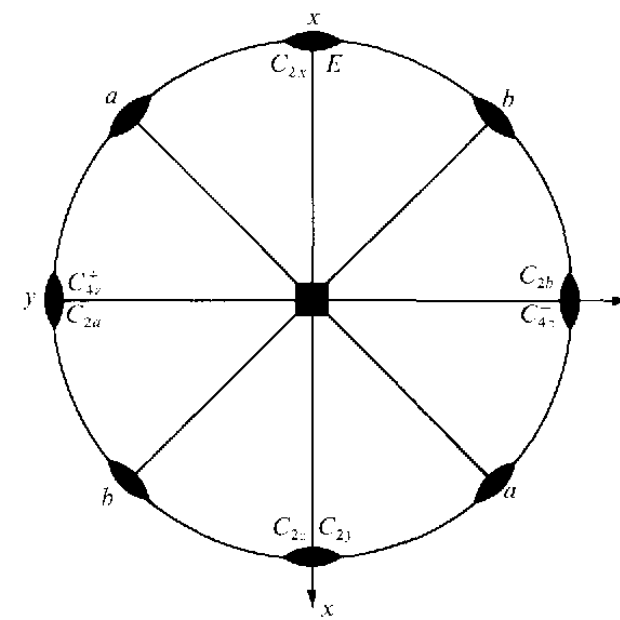
\includegraphics[width=0.60\textwidth]{figures/fig1_1.png}
\caption{Symmetry elements: triclinic, monoclinic, orthorhombic, and tetragonal systems. The point groups in these systems are subgroups of $m3m$ ($O_{h}$) and so the same notation is used. $x$, $y$, $z$ form a right-handed set of axes. The labels of the symmetry operations are placed on the figure in the position to which the letter $E$ is taken by that operation.}
\end{figure}

operator can be separately identified. The notation for the proper rotations has already been indicated in the classification of the proper point groups; the identification is made complete by reference to Tables 1.2 and 1.3 and to Figs. 1.1–1.3.

\begin{figure}[H]
\centering
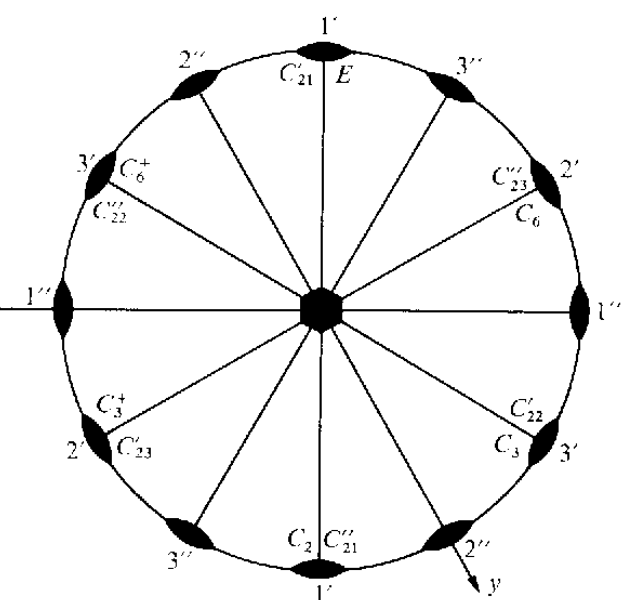
\includegraphics[width=0.60\textwidth]{figures/fig1_2.png}
\caption{Symmetry elements: trigonal and hexagonal systems. The $z$-axis is vertically upwards, out of the page. The labels of the symmetry operations are placed on the figure in the position to which the letter $E$ is taken by that operation.}
\end{figure}

Many results depend for their usefulness on a complete identification of the symmetry elements present and so we shall give some attention to this matter. To identify the symmetry elements for point groups belonging to most crystal systems it is possible to use a plane figure such as a stereogram, and we do this for the triclinic, monoclinic, orthorhombic, and tetragonal systems in Fig. 1.1 and for the trigonal and hexagonal systems in Fig. 1.2. Two-sided paper models have been used by Schiff (1954) to help visualize the different non-cubic point groups. However, for the cubic system it is easier to identify the symmetry elements from the figure of a cube; this is done in Fig. 1.3. $C_{nr}^{+}$ is an anti-clockwise rotation of the points of space through $2\pi/n$ radians about the axis labelled by $r$ on the figure in question. $C_{nr}^{-}$ is a clockwise rotation of the points of space through $2\pi/n$ radians about the same axis. $E$ is the identity and $I$ is the inversion. In Table 1.2 the operators that appear in a given system are listed for each of the seven crystal systems; in each part of the table there are two columns, the elements in the right-hand column being the product of $I$ with the corresponding elements in the left-hand column. The elements given in this table are those that appear when the appropriate point group is in the standard setting with respect to the $x$, $y$, and $z$ axes of the figure. Non-standard settings of certain point groups will sometimes have to be used, but since each element is given a definite label this will be no cause for confusion. It should be noticed that reflection planes are always denoted by $\sigma$ and other rotation reflections by $S$; it should also be noted that in the notation that we are using $IC_{2} = \sigma$, $IC_{3}^{+} = S_{6}^{-}$, $IC_{4}^{+} = S_{4}^{-}$, $IC_{6}^{+} = S_{3}^{-}$ (that is, $IC_{3}^{+} = S_{6}^{-}$, and so on). This is because $S_{n}^{+}$ denotes an anti-clockwise rotation by $2\pi/n$ followed by a reflection in the plane perpendicular to the rotation and hence $IC_{n}^{+} = \sigma C_{2}C_{n}^{+} = \sigma(C_{n}^{+})^{n+2} = (S_{2n}^{-})^{n+2}$.

A final and very important point, which we have mentioned earlier, must be stressed and that is that when dealing with a point-group operator it will be interpreted always as an \textit{active} operator moving the points of space and leaving the axes fixed; similarly, when dealing with a space-group operator written in the form $\{R \,|\, \mathbf{v}\}$ (see section 1.5) it too will be interpreted as active.

\begin{figure}[H]
\centering
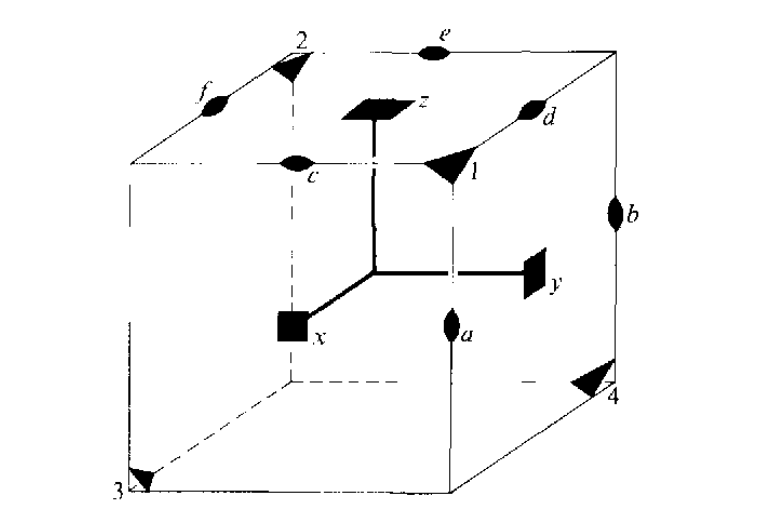
\includegraphics[width=0.60\textwidth]{figures/fig1_3.png}
\caption{Symmetry elements: cubic system (Altmann and Bradley 1963\textit{b}).}
\end{figure}

In Table 1.3 we identify the symmetry operations that are present in each of the 32 crystallographic point groups. The point groups are arranged according to the seven crystal systems and all the elements of each point group are given. Wherever a point group has a principal axis this axis is set in the $Oz$ direction and this is called the \textit{standard setting}, but of course many other settings are possible. In Fig. 1.4 are shown stereograms for the 32 crystallographic point groups; for details of the theory of stereographic projection see, for example, Phillips (1963). In any given crystal system the point group that contains the largest number of symmetry operations is called the \textit{holosymmetric} point group of that system.

\textit{The multiplication of point-group operations}

The result of the application of two point-group operations in succession is easily obtained with the help of a stereogram for all point groups other than the cubic

\begin{figure}[H]
\centering
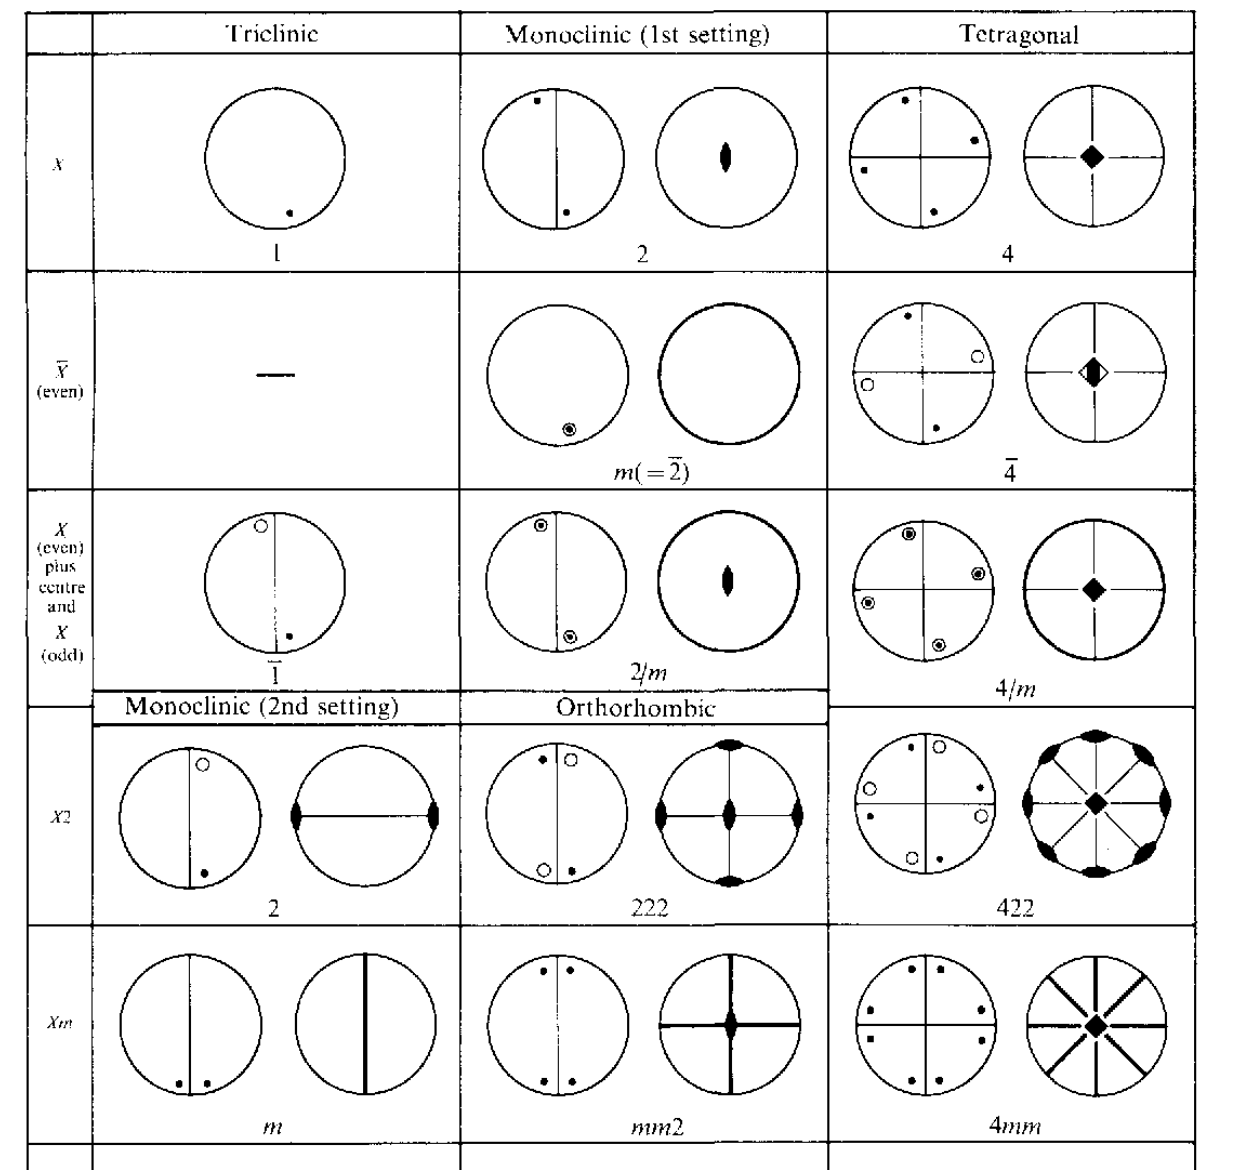
\includegraphics[width=0.98\textwidth]{figures/fig1_4a.png}
\end{figure}
\begin{figure}[H]
\centering
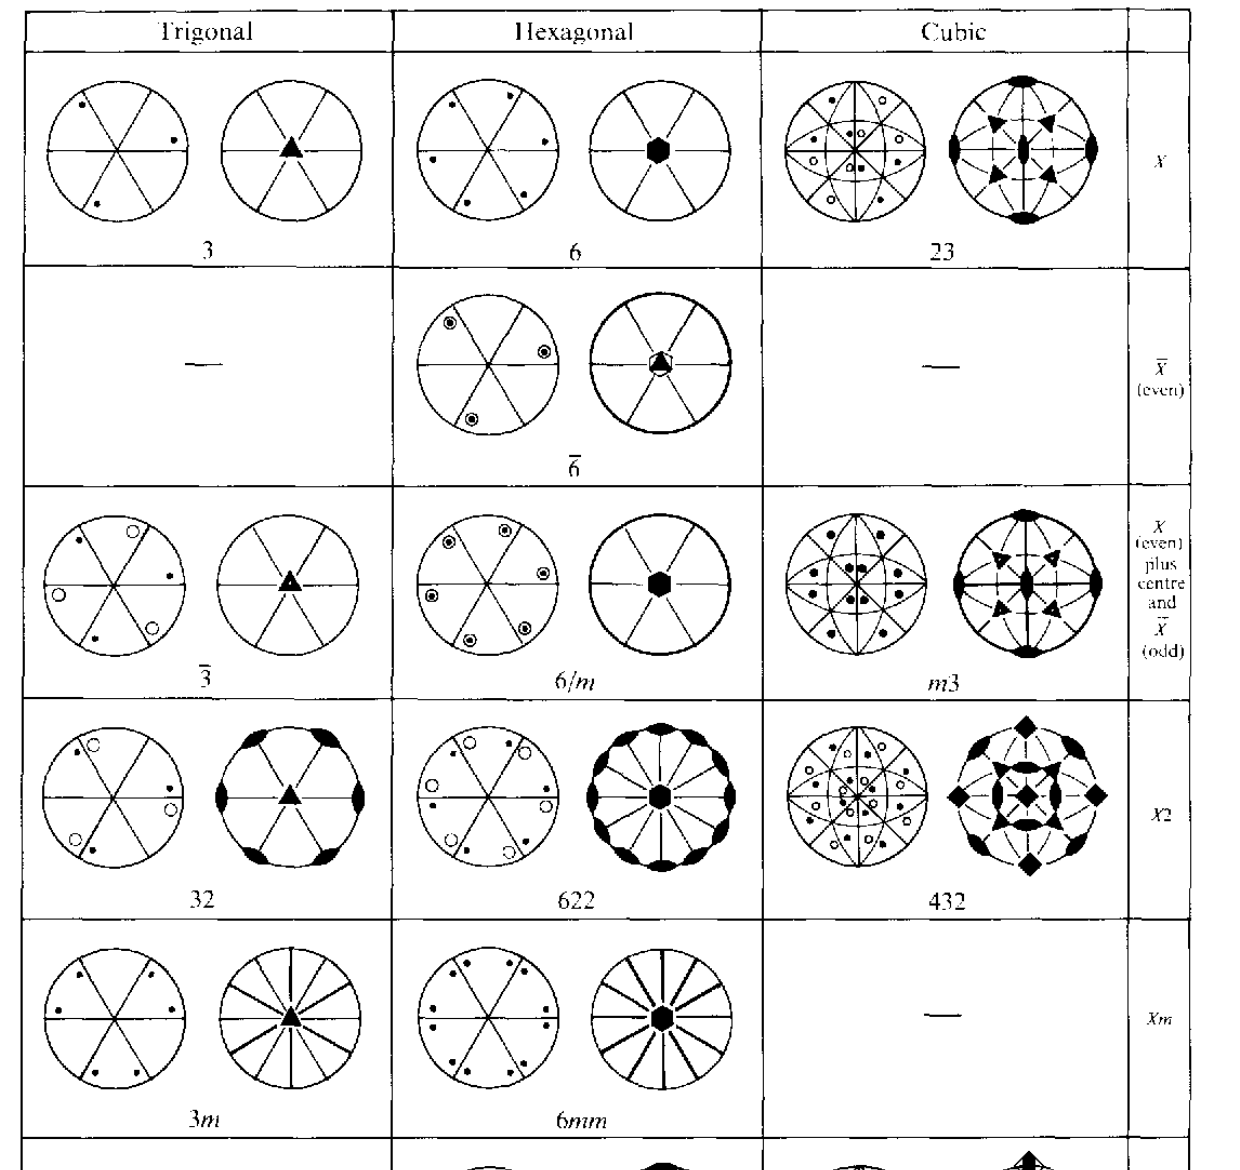
\includegraphics[width=0.98\textwidth]{figures/fig1_4b.png}
\caption{Stereograms of poles of general equivalent directions and symmetry elements of each of the 32 point groups ($z$-axis normal to the paper in all drawings; for $m3$ and $m3m$ only half the points are shown) (Henry and Lonsdale 1965).}
\end{figure}

\begin{minipage}{\textwidth}
\centering\textbf{TABLE 1.3}
\textit{The 32 point groups}

\centering
\begin{tabular}{|c|c|c|p{0.58\textwidth}|}
\hline
No. & Label &  & Elements \\ \hline
\textit{Triclinic} &  &  &  \\ \hline
1 & $1$ & $C_{1}$ & $E$ \\ \hline
2 & $\bar{1}$ & $C_{i}$ & $E, I$ \\ \hline
\textit{Monoclinic} &  &  &  \\ \hline
3 & $2$ & $C_{2}$ & $E, C_{2z}$ \\ \hline
4 & $m$ & $C_{s}, C_{1h}$ & $E, \sigma_{z}$ \\ \hline
5 & $2/m$ & $C_{2h}$ & $E, C_{2z}, I, \sigma_{z}$ \\ \hline
\textit{Orthorhombic} &  &  &  \\ \hline
6 & $222$ & $D_{2}$ & $E, C_{2x}, C_{2y}, C_{2z}$ \\ \hline
7 & $mm2$ & $C_{2v}$ & $E, C_{2z}, \sigma_{x}, \sigma_{y}$ \\ \hline
8 & $mmm$ & $D_{2h}$ & $E, C_{2x}, C_{2y}, C_{2z}, I, \sigma_{x}, \sigma_{y}, \sigma_{z}$ \\ \hline
\textit{Tetragonal} &  &  &  \\ \hline
9 & $4$ & $C_{4}$ & $E, C_{4z}^{+}, C_{4z}^{-}, C_{2z}$ \\ \hline
10 & $\bar{4}$ & $S_{4}$ & $E, S_{4z}^{+}, S_{4z}^{-}, C_{2z}$ \\ \hline
11 & $4/m$ & $C_{4h}$ & $E, C_{4z}^{+}, C_{4z}^{-}, C_{2z}, I, S_{4z}^{-}, S_{4z}^{+}, \sigma_{z}$ \\ \hline
12 & $422$ & $D_{4}$ & $E, C_{4z}^{+}, C_{4z}^{-}, C_{2z}, C_{2x}, C_{2y}, C_{2a}, C_{2b}$ \\ \hline
13 & $4mm$ & $C_{4v}$ & $E, C_{4z}^{+}, C_{4z}^{-}, C_{2z}, \sigma_{x}, \sigma_{y}, \sigma_{da}, \sigma_{db}$ \\ \hline
14 & $\bar{4}2m$ & $D_{2d}$ & $E, S_{4z}^{+}, S_{4z}^{-}, C_{2z}, C_{2x}, C_{2y}, \sigma_{da}, \sigma_{db}$ \\ \hline
15 & $4/mmm$ & $D_{4h}$ & $E, C_{4z}^{+}, C_{4z}^{-}, C_{2z}, C_{2x}, C_{2y}, C_{2a}, C_{2b}$\newline $I, S_{4z}^{-}, S_{4z}^{+}, \sigma_{z}, \sigma_{x}, \sigma_{y}, \sigma_{da}, \sigma_{db}$ \\ \hline
\textit{Trigonal} &  &  &  \\ \hline
16 & $3$ & $C_{3}$ & $E, C_{3}^{+}, C_{3}^{-}$ \\ \hline
17 & $\bar{3}$ & $C_{3i}$ & $E, C_{3}^{+}, C_{3}^{-}, I, S_{6}^{-}, S_{6}^{+}$ \\ \hline
18 & $32$ & $D_{3}$ & $E, C_{3}^{+}, C_{3}^{-}, C'_{21}, C'_{22}, C'_{23}$ \\ \hline
19 & $3m$ & $C_{3v}$ & $E, C_{3}^{+}, C_{3}^{-}, \sigma_{d1}, \sigma_{d2}, \sigma_{d3}$ \\ \hline
20 & $\bar{3}m$ & $D_{3d}$ & $E, C_{3}^{+}, C_{3}^{-}, C'_{21}, C'_{22}, C'_{23}, I, S_{6}^{-}, S_{6}^{+}, \sigma_{d1}, \sigma_{d2}, \sigma_{d3}$ \\ \hline
\textit{Hexagonal} &  &  &  \\ \hline
21 & $6$ & $C_{6}$ & $E, C_{6}^{+}, C_{6}^{-}, C_{3}^{+}, C_{3}^{-}, C_{2}$ \\ \hline
22 & $\bar{6}$ & $C_{3h}$ & $E, S_{3}^{-}, S_{3}^{+}, C_{3}^{+}, C_{3}^{-}, \sigma_{h}$ \\ \hline
23 & $6/m$ & $C_{6h}$ & $E, C_{6}^{+}, C_{6}^{-}, C_{3}^{+}, C_{3}^{-}, C_{2}, I, S_{3}^{-}, S_{3}^{+}, S_{6}^{-}, S_{6}^{+}, \sigma_{h}$ \\ \hline
24 & $622$ & $D_{6}$ & $E, C_{6}^{+}, C_{6}^{-}, C_{3}^{+}, C_{3}^{-}, C_{2}, C'_{21}, C'_{22}, C'_{23}, C''_{21}, C''_{22}, C''_{23}$ \\ \hline
25 & $6mm$ & $C_{6v}$ & $E, C_{6}^{+}, C_{6}^{-}, C_{3}^{+}, C_{3}^{-}, C_{2}, \sigma_{d1}, \sigma_{d2}, \sigma_{d3}, \sigma_{v1}, \sigma_{v2}, \sigma_{v3}$ \\ \hline
26 & $\bar{6}2m$ & $D_{3h}$ & $E, S_{3}^{-}, S_{3}^{+}, C_{3}^{+}, C_{3}^{-}, \sigma_{h}, C'_{21}, C'_{22}, C'_{23}, \sigma_{v1}, \sigma_{v2}, \sigma_{v3}$ \\ \hline
27 & $6/mmm$ & $D_{6h}$ & $E, C_{6}^{+}, C_{6}^{-}, C_{3}^{+}, C_{3}^{-}, C_{2}, C'_{21}, C'_{22}, C'_{23}, C''_{21}, C''_{22}, C''_{23}$\newline $I, S_{3}^{-}, S_{3}^{+}, S_{6}^{-}, S_{6}^{+}, \sigma_{h}, \sigma_{d1}, \sigma_{d2}, \sigma_{d3}, \sigma_{v1}, \sigma_{v2}, \sigma_{v3}$ \\ \hline
\textit{Cubic} &  &  &  \\ \hline
28 & $23$ & $T$ & $E, C_{2m}, C_{3j}^{+}, C_{3j}^{-}$ \\ \hline
29 & $m3$ & $T_{h}$ & $E, C_{2m}, C_{3j}^{+}, C_{3j}^{-}, I, \sigma_{m}, S_{6j}^{-}, S_{6j}^{+}$ \\ \hline
30 & $432$ & $O$ & $E, C_{2m}, C_{3j}^{+}, C_{3j}^{-}, C_{2p}, C_{4m}^{+}, C_{4m}^{-}$ \\ \hline
31 & $\bar{4}3m$ & $T_{d}$ & $E, C_{2m}, C_{3j}^{+}, C_{3j}^{-}, \sigma_{dp}, S_{4m}^{-}, S_{4m}^{+}$ \\ \hline
32 & $m3m$ & $O_{h}$ & $E, C_{2m}, C_{3j}^{+}, C_{3j}^{-}, C_{2p}, C_{4m}^{+}, C_{4m}^{-}$\newline $I, \sigma_{m}, S_{6j}^{-}, S_{6j}^{+}, \sigma_{dp}, S_{4m}^{-}, S_{4m}^{+}$ \\ \hline
\end{tabular}
\end{minipage}
\medskip

\textit{Notes to Table 1.3}

\begin{quote}(i) The arbitrary numbers in column 1 are those of Koster, Dimmock, Wheeler, and Statz (1963). (ii) The labels of the symmetry operations can be identified from Figs. 1.1–1.3; $j = 1, 2, 3,$ and $4$; $m = x, y,$ and $z$; $p = a, b, c, d, e,$ and $f$. (iii) The principal axes have been set in the $Oz$ direction but there are still possible alternative settings for some of the point groups, for example $\bar{4}2m$ ($D_{2d}$) may contain the elements, $E$, $S_{4z}^{-}$, $C_{2z}$, $S_{4z}^{+}$, $\sigma_{x}$, $\sigma_{y}$, $C_{2a}$, and $C_{2b}$; sometimes alternatives of this kind are important when one considers the space groups (see Chapter 3).\end{quote}

groups. For example, the multiplication $C_{2x}C_{4z}^{+} = C_{2b}$ is illustrated in Fig. 1.5, in which a dot represents a point above the plane of the drawing and a circle a point below the plane of the drawing. The point $A$ is taken into the point $B$ by the operation $C_{4z}^{-}$; $B$ is in turn taken into the point $C$ by the operation $C_{2x}$. The result is the operation that takes $A$ directly into the point $C$, namely $C_{2b}$, as can be seen from Fig 1.1.

\begin{figure}[H]
\centering
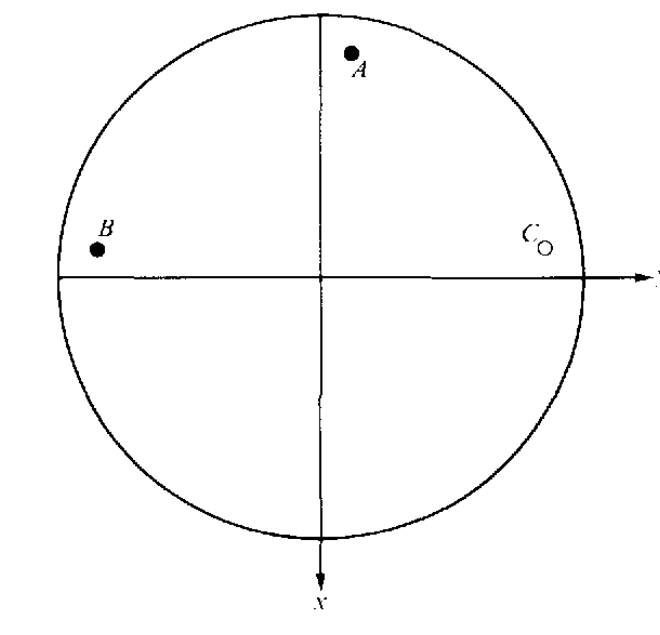
\includegraphics[width=0.60\textwidth]{figures/fig1_5.png}
\caption{}
\end{figure}

For a cubic point group the easiest way to obtain the group multiplication table is to use the Jones' faithful representation of the operators given in Table 1.4(a). The Jones symbol for the operator $R$ is just the vector formed by the action of the operator $R$ on the vector $(x, y, z)$; these symbols may be recognized as the coordinates of equivalent positions in the unit cells of symmorphic cubic and hexagonal space groups in Table 4.3 of Volume 1 of the \textit{International tables for X-ray crystallography} (Henry and Lonsdale 1965). If $(x, y, z)$ is a vector referred to a basis of unit vectors $\mathbf{i}$, $\mathbf{j}$, and $\mathbf{k}$ along the coordinate axes, then, for example, $C_{4z}^{+}x\mathbf{i} = x\mathbf{j}$, $C_{4z}^{+}y\mathbf{j} = -y\mathbf{i}$, and $C_{4z}^{+}z\mathbf{k} = z\mathbf{k}$, so that we may write $C_{4z}^{+}(x, y, z) = (-y, x, z)$ or

\begin{equation*}
C_{4z}^{+}(x\mathbf{i} + y\mathbf{j} + z\mathbf{k}) = (-y\mathbf{i} + x\mathbf{j} + z\mathbf{k}) \tag{1.4.8}
\end{equation*}

and the Jones' faithful representation of $C_{4z}^{+}$ is then written as $(\bar{y}xz)$. The matrix representing $C_{4z}^{+}$ with respect to the basis consisting of the row vector $\langle \mathbf{i}, \mathbf{j}, \mathbf{k}|$ is

\begin{equation*}
\mathbf{D}(C_{4z}^{+}) = \begin{pmatrix} 0 & -1 & 0 \\ 1 & 0 & 0 \\ 0 & 0 & 1 \end{pmatrix} \tag{1.4.9}
\end{equation*}
 and thus the Jones' symbol is an abbreviation for this matrix representative. Equation (1.4.9) follows from the fact that

\begin{equation*}
C_{4z}^{+}\langle \mathbf{i}, \mathbf{j}, \mathbf{k}| = \langle \mathbf{i}, \mathbf{j}, \mathbf{k}| \begin{pmatrix} 0 & -1 & 0 \\ 1 & 0 & 0 \\ 0 & 0 & 1 \end{pmatrix}, \tag{1.4.10}
\end{equation*}

which illustrates why $D$ is a faithful representation.

The multiplication rule for these symbols is easily derived from the multiplication rule for matrices. Thus, for example,

\begin{equation*}
(zxy)(\bar{y}xz) = \begin{pmatrix} 0 & 0 & 1 \\ 1 & 0 & 0 \\ 0 & 1 & 0 \end{pmatrix} \begin{pmatrix} 0 & -1 & 0 \\ 1 & 0 & 0 \\ 0 & 0 & 1 \end{pmatrix} = \begin{pmatrix} 0 & 0 & 1 \\ 0 & -1 & 0 \\ 1 & 0 & 0 \end{pmatrix} = (z\bar{y}x). \tag{1.4.11}
\end{equation*}

There is no need to write out the matrices in full, for

\begin{equation*}
(zxy)(\bar{y}xz) = (z'x'y'), \quad \text{where} \quad (x'y'z') = (\bar{y}xz),
\end{equation*}

so that

\begin{equation*}
(z'x'y') = (z\bar{y}x).
\end{equation*}

Equation (1.4.11) is a representation equation reading

\begin{equation*}
\mathbf{D}(C_{31}^{+})\mathbf{D}(C_{4z}^{+}) = \mathbf{D}(C_{2c}) \tag{1.4.12}
\end{equation*}

as can be seen from Table 1.4(a) in which the Jones' faithful representation symbol is given for each of the 48 cubic point-group operations. Since $D$ is a faithful representation it follows at once that $C_{31}^{+}C_{4z}^{+} = C_{2c}$. The Jones' symbols given in Table 1.4(a) can also be used for the elements of tetragonal or orthorhombic point groups and for monoclinic or triclinic point groups where the vector $(x, y, z)$ is referred to a basis of unit vectors $\mathbf{i}$, $\mathbf{j}$, and $\mathbf{k}$ parallel to the axes of the crystal. A similar set of symbols in Table 1.4(b) gives the effect of the operations of a hexagonal or trigonal point group on a vector $(x, y, z)$ where $(x, y, z)$ is referred to a basis of unit vectors $\mathbf{i}$, $\mathbf{j}$, and $\mathbf{k}$, where $\mathbf{i}$ and $\mathbf{j}$ are at 120\textdegree  to each other and are in the plane normal to $\mathbf{k}$.

In Tables 1.5 and 1.6 we give the group multiplication tables for the two point groups 432 ($O$) and 622 ($D_{6}$) (Belov 1957\textit{b}, Belov and Tarkhova 1960, Hurley 1966, Koptsik 1966). These two point groups consist only of pure rotations; all those other

\begin{minipage}{\textwidth}
\centering\textbf{TABLE 1.4}
\textit{Jones' faithful representation symbols}

\noindent\resizebox{\textwidth}{!}{
\centering
\begin{tabular}{|l|l|l|l|l|l|l|l|}
\hline
(a) \textit{Cubic} &  &  &  &  &  & (b) \textit{Hexagonal} &  \\ \hline
$E$ & $xyz$ & $I$ & $\bar{x}\bar{y}\bar{z}$ & $C_{4x}^{+}$ & $x\bar{z}y$ & $E$ & $x, y, z$ \\ \hline
$C_{2x}$ & $x\bar{y}\bar{z}$ & $\sigma_{x}$ & $\bar{x}yz$ & $C_{4y}^{+}$ & $zy\bar{x}$ & $C_{6}^{+}$ & $x-y, x, z$ \\ \hline
$C_{2y}$ & $\bar{x}y\bar{z}$ & $\sigma_{y}$ & $x\bar{y}z$ & $C_{4z}^{+}$ & $\bar{y}xz$ & $C_{3}^{+}$ & $\bar{y}, x-y, z$ \\ \hline
$C_{2z}$ & $\bar{x}\bar{y}z$ & $\sigma_{z}$ & $xy\bar{z}$ & $C_{4x}^{-}$ & $xz\bar{y}$ & $C_{2}$ & $\bar{x}, \bar{y}, z$ \\ \hline
$C_{31}^{+}$ & $zxy$ & $S_{61}^{-}$ & $\bar{z}\bar{x}\bar{y}$ & $C_{4y}^{-}$ & $\bar{z}yx$ & $C_{3}^{-}$ & $y-x, \bar{x}, z$ \\ \hline
$C_{32}^{+}$ & $\bar{z}x\bar{y}$ & $S_{62}^{-}$ & $z\bar{x}y$ & $C_{4z}^{-}$ & $y\bar{x}z$ & $C_{6}^{-}$ & $y, y-x, z$ \\ \hline
$C_{33}^{+}$ & $\bar{z}\bar{x}y$ & $S_{63}^{-}$ & $zx\bar{y}$ & $C_{2a}$ & $yx\bar{z}$ & $C'_{21}$ & $y-x, y, \bar{z}$ \\ \hline
$C_{34}^{+}$ & $z\bar{x}\bar{y}$ & $S_{64}^{-}$ & $\bar{z}xy$ & $C_{2b}$ & $\bar{y}\bar{x}z$ & $C'_{22}$ & $x, x-y, \bar{z}$ \\ \hline
$C_{31}^{-}$ & $yzx$ & $S_{61}^{+}$ & $\bar{y}\bar{z}\bar{x}$ & $C_{2c}$ & $z\bar{y}x$ & $C'_{23}$ & $\bar{y}, \bar{x}, \bar{z}$ \\ \hline
$C_{32}^{-}$ & $y\bar{z}\bar{x}$ & $S_{62}^{+}$ & $\bar{y}zx$ & $C_{2d}$ & $\bar{z}\bar{y}\bar{x}$ & $C''_{21}$ & $x-y, \bar{y}, \bar{z}$ \\ \hline
$C_{33}^{-}$ & $\bar{y}z\bar{x}$ & $S_{63}^{+}$ & $yz\bar{x}$ & $C_{2e}$ & $\bar{x}zy$ & $C''_{22}$ & $\bar{x}, y-x, \bar{z}$ \\ \hline
$C_{34}^{-}$ & $\bar{y}\bar{z}x$ & $S_{64}^{+}$ & $yzx$ & $C_{2f}$ & $\bar{x}\bar{z}\bar{y}$ & $C''_{23}$ & $y, x, \bar{z}$ \\ \hline
$S_{4x}^{-}$ & $\bar{x}z\bar{y}$ & $\sigma_{da}$ & $\bar{y}\bar{x}z$ & $\sigma_{v1}$ & $y-x, y, z$ &  &  \\ \hline
$S_{4y}^{-}$ & $\bar{z}yx$ & $\sigma_{db}$ & $yx\bar{z}$ & $\sigma_{v2}$ & $x, x-y, z$ &  &  \\ \hline
$S_{4z}^{-}$ & $\bar{y}\bar{x}\bar{z}$ & $\sigma_{dc}$ & $\bar{z}y\bar{x}$ & $\sigma_{v3}$ & $\bar{y}, \bar{x}, z$ &  &  \\ \hline
$S_{4x}^{+}$ & $\bar{x}\bar{z}y$ & $\sigma_{dd}$ & $zyx$ &  &  &  &  \\ \hline
$S_{4y}^{+}$ & $z\bar{y}\bar{x}$ & $\sigma_{de}$ & $x\bar{z}\bar{y}$ &  &  &  &  \\ \hline
$S_{4z}^{+}$ & $\bar{y}x\bar{z}$ & $\sigma_{df}$ & $xzy$ &  &  &  &  \\ \hline
\end{tabular}
}
\end{minipage}
\medskip

\textit{Notes to Table 1.4}

\begin{quote}(i) As mentioned in the text the symbol next to an (active) operator $R$ is just the vector formed from the vector $(x, y, z)$ by $R$. (ii) In (a) the unit vectors $\mathbf{i}$, $\mathbf{j}$, and $\mathbf{k}$ are mutually orthogonal and are along the $x$, $y$, and $z$ axes of Fig. 1.1. In (b) the unit vectors $\mathbf{i}$, $\mathbf{j}$, and $\mathbf{k}$ are along the $x$, $y$, and $z$ axes of Fig. 1.2; therefore $\mathbf{i}$ and $\mathbf{j}$ are at 120\textdegree  to each other and are in the plane normal to $\mathbf{k}$. (iii) Thus, for example, $C_{4z}^{-}$ has the symbol $(y\bar{x}z)$  so that

\begin{equation*}
C_{4z}^{-}(x\mathbf{i} + y\mathbf{j} + z\mathbf{k}) = (y\mathbf{i} - x\mathbf{j} + z\mathbf{k}).
\end{equation*}

(iv) (a) is also to be used for the tetragonal, orthorhombic, monoclinic, and triclinic systems; for the monoclinic and triclinic systems $\mathbf{i}$, $\mathbf{j}$, and $\mathbf{k}$ are parallel to the axes of the crystal. (b) is also to be used for the trigonal system. (v) The symbols in (a) and (b) may be recognized as simply the coordinates of equivalent positions in the unit cells of symmorphic cubic and hexagonal space groups in Table 4.3 of Volume 1 of the \textit{International tables for X-ray crystallography} (Henry and Lonsdale 1965).\end{quote}

point groups that consist only of pure rotations are subgroups of one or other of these two point groups. Each of those remaining point groups that contain operations that are not pure rotations is simply related to one of the point groups consisting of pure rotations only. Thus, from Tables 1.5 and 1.6 it is possible to obtain very quickly the group multiplication table of any of the 32 point groups.

\section{Space groups}

Before discussing the definition of a space group it is desirable to consider what is meant by a \textit{Bravais lattice}. A lattice is a collection of mathematical points arranged in such a way that each lattice point has the same environment in the same orientation. With reference to crystalline solids, the atoms or molecules of which such a solid is composed are found to be arranged in a regular manner (Haüy 1815\textit{a}–\textit{d}). That is, within a crystalline solid there is a set of mathematical lattice points. If a Maxwell demon were to view such a crystal from any one of these points he would see an

\begin{minipage}{\textwidth}
\centering\textbf{TABLE 1.5}
\textit{The group multiplication table for the point group} 432 ($O$)

\noindent\resizebox{\textwidth}{!}{
\centering
\begin{tabular}{|l|l|l|l|l|l|l|l|l|l|l|l|l|l|l|l|l|l|l|l|l|l|l|l|l|}
\hline
 & $E$ & $C_{2x}$ & $C_{2y}$ & $C_{2z}$ & $C_{4-}^{}$ & $C_{4-}^{}$ & $C_{4-}^{}$ & $C_{4+}^{}$ & $C_{4+}^{}$ & $C_{4+}^{}$ & $C_{3-}^{}$ & $C_{3-}^{}$ & $C_{3-}^{}$ & $C_{3-}^{}$ & $C_{3+}^{}$ & $C_{3+}^{}$ & $C_{3+}^{}$ & $C_{3+}^{}$ & $C_{2a}$ & $C_{2b}$ & $C_{2c}$ & $C_{2d}$ & $C_{2e}$ & $C_{2f}$ \\ \hline
$E$ & $E$ & $C_{2x}$ & $C_{2y}$ & $C_{2z}$ & $C_{4-}^{}$ & $C_{4-}^{}$ & $C_{4-}^{}$ & $C_{4+}^{}$ & $C_{4+}^{}$ & $C_{4+}^{}$ & $C_{3-}^{}$ & $C_{3-}^{}$ & $C_{3-}^{}$ & $C_{3-}^{}$ & $C_{3+}^{}$ & $C_{3+}^{}$ & $C_{3+}^{}$ & $C_{3+}^{}$ & $C_{2a}$ & $C_{2b}$ & $C_{2c}$ & $C_{2d}$ & $C_{2e}$ & $C_{2f}$ \\ \hline
$C_{2x}$ & $C_{2x}$ & $E$ & $C_{2z}$ & $C_{2y}$ & $C_{4+}^{}$ & $C_{2d}$ & $C_{2a}$ & $C_{4-}^{}$ & $C_{2c}$ & $C_{2b}$ & $C_{3-}^{}$ & $C_{3-}^{}$ & $C_{3-}^{}$ & $C_{3-}^{}$ & $C_{3+}^{}$ & $C_{3+}^{}$ & $C_{3+}^{}$ & $C_{3+}^{}$ & $C_{4-}^{}$ & $C_{4+}^{}$ & $C_{4+}^{}$ & $C_{4-}^{}$ & $C_{2f}$ & $C_{2e}$ \\ \hline
$C_{2y}$ & $C_{2y}$ & $C_{2z}$ & $E$ & $C_{2x}$ & $C_{2e}$ & $C_{4+}^{}$ & $C_{2b}$ & $C_{2f}$ & $C_{4-}^{}$ & $C_{2a}$ & $C_{3-}^{}$ & $C_{3-}^{}$ & $C_{3-}^{}$ & $C_{3-}^{}$ & $C_{3+}^{}$ & $C_{3+}^{}$ & $C_{3+}^{}$ & $C_{3+}^{}$ & $C_{4+}^{}$ & $C_{4-}^{}$ & $C_{2d}$ & $C_{2c}$ & $C_{4-}^{}$ & $C_{4+}^{}$ \\ \hline
$C_{2z}$ & $C_{2z}$ & $C_{2y}$ & $C_{2x}$ & $E$ & $C_{2f}$ & $C_{2c}$ & $C_{4+}^{}$ & $C_{2e}$ & $C_{2d}$ & $C_{4-}^{}$ & $C_{3-}^{}$ & $C_{3-}^{}$ & $C_{3-}^{}$ & $C_{3-}^{}$ & $C_{3+}^{}$ & $C_{3+}^{}$ & $C_{3+}^{}$ & $C_{3+}^{}$ & $C_{2b}$ & $C_{2a}$ & $C_{4-}^{}$ & $C_{4+}^{}$ & $C_{4+}^{}$ & $C_{4-}^{}$ \\ \hline
$C_{4-}^{}$ & $C_{4-}^{}$ & $C_{4+}^{}$ & $C_{2f}$ & $C_{2e}$ & $C_{2x}$ & $C_{3+}^{}$ & $C_{3-}^{}$ & $E$ & $C_{3+}^{}$ & $C_{3-}^{}$ & $C_{2a}$ & $C_{4-}^{}$ & $C_{2b}$ & $C_{4+}^{}$ & $C_{4+}^{}$ & $C_{2d}$ & $C_{4-}^{}$ & $C_{2c}$ & $C_{3-}^{}$ & $C_{3-}^{}$ & $C_{3+}^{}$ & $C_{3+}^{}$ & $C_{2y}$ & $C_{2z}$ \\ \hline
$C_{4-}^{}$ & $C_{4-}^{}$ & $C_{2c}$ & $C_{4+}^{}$ & $C_{2d}$ & $C_{3-}^{}$ & $C_{2y}$ & $C_{3+}^{}$ & $C_{3-}^{}$ & $E$ & $C_{3+}^{}$ & $C_{2e}$ & $C_{4+}^{}$ & $C_{4-}^{}$ & $C_{2f}$ & $C_{4+}^{}$ & $C_{2a}$ & $C_{2b}$ & $C_{4-}^{}$ & $C_{3+}^{}$ & $C_{3+}^{}$ & $C_{2z}$ & $C_{2x}$ & $C_{3-}^{}$ & $C_{3-}^{}$ \\ \hline
$C_{4-}^{}$ & $C_{4-}^{}$ & $C_{2b}$ & $C_{2a}$ & $C_{4+}^{}$ & $C_{3+}^{}$ & $C_{3-}^{}$ & $C_{2z}$ & $C_{3+}^{}$ & $C_{3-}^{}$ & $E$ & $C_{2c}$ & $C_{2d}$ & $C_{4+}^{}$ & $C_{4-}^{}$ & $C_{4+}^{}$ & $C_{4-}^{}$ & $C_{2e}$ & $C_{2f}$ & $C_{2x}$ & $C_{2y}$ & $C_{3-}^{}$ & $C_{3-}^{}$ & $C_{3+}^{}$ & $C_{3+}^{}$ \\ \hline
$C_{4+}^{}$ & $C_{4+}^{}$ & $C_{4-}^{}$ & $C_{2e}$ & $C_{2f}$ & $E$ & $C_{3+}^{}$ & $C_{3-}^{}$ & $C_{2x}$ & $C_{3+}^{}$ & $C_{3-}^{}$ & $C_{4-}^{}$ & $C_{2a}$ & $C_{4+}^{}$ & $C_{2b}$ & $C_{2c}$ & $C_{4-}^{}$ & $C_{2d}$ & $C_{4+}^{}$ & $C_{3-}^{}$ & $C_{3-}^{}$ & $C_{3+}^{}$ & $C_{3+}^{}$ & $C_{2z}$ & $C_{2y}$ \\ \hline
$C_{4+}^{}$ & $C_{4+}^{}$ & $C_{2d}$ & $C_{4-}^{}$ & $C_{2c}$ & $C_{3-}^{}$ & $E$ & $C_{3+}^{}$ & $C_{3-}^{}$ & $C_{2y}$ & $C_{3+}^{}$ & $C_{4-}^{}$ & $C_{2f}$ & $C_{2e}$ & $C_{4+}^{}$ & $C_{2a}$ & $C_{4+}^{}$ & $C_{4-}^{}$ & $C_{2b}$ & $C_{3+}^{}$ & $C_{3+}^{}$ & $C_{2x}$ & $C_{2z}$ & $C_{3-}^{}$ & $C_{3-}^{}$ \\ \hline
$C_{4+}^{}$ & $C_{4+}^{}$ & $C_{2a}$ & $C_{2b}$ & $C_{4-}^{}$ & $C_{3+}^{}$ & $C_{3-}^{}$ & $E$ & $C_{3+}^{}$ & $C_{3-}^{}$ & $C_{2z}$ & $C_{4-}^{}$ & $C_{4+}^{}$ & $C_{2d}$ & $C_{2c}$ & $C_{2e}$ & $C_{2f}$ & $C_{4+}^{}$ & $C_{4-}^{}$ & $C_{2y}$ & $C_{2x}$ & $C_{3-}^{}$ & $C_{3-}^{}$ & $C_{3+}^{}$ & $C_{3+}^{}$ \\ \hline
$C_{3-}^{}$ & $C_{3-}^{}$ & $C_{3-}^{}$ & $C_{3-}^{}$ & $C_{3-}^{}$ & $C_{2c}$ & $C_{2a}$ & $C_{2e}$ & $C_{4-}^{}$ & $C_{4-}^{}$ & $C_{4-}^{}$ & $C_{3+}^{}$ & $C_{3+}^{}$ & $C_{3+}^{}$ & $C_{3+}^{}$ & $E$ & $C_{2x}$ & $C_{2y}$ & $C_{2z}$ & $C_{4+}^{}$ & $C_{2f}$ & $C_{4+}^{}$ & $C_{2b}$ & $C_{4+}^{}$ & $C_{2d}$ \\ \hline
$C_{3-}^{}$ & $C_{3-}^{}$ & $C_{3-}^{}$ & $C_{3-}^{}$ & $C_{3-}^{}$ & $C_{4+}^{}$ & $C_{4-}^{}$ & $C_{2f}$ & $C_{2d}$ & $C_{2a}$ & $C_{4+}^{}$ & $C_{3+}^{}$ & $C_{3+}^{}$ & $C_{3+}^{}$ & $C_{3+}^{}$ & $C_{2x}$ & $E$ & $C_{2z}$ & $C_{2y}$ & $C_{4-}^{}$ & $C_{2e}$ & $C_{2b}$ & $C_{4+}^{}$ & $C_{2c}$ & $C_{4-}^{}$ \\ \hline
$C_{3-}^{}$ & $C_{3-}^{}$ & $C_{3-}^{}$ & $C_{3-}^{}$ & $C_{3-}^{}$ & $C_{2d}$ & $C_{4+}^{}$ & $C_{4-}^{}$ & $C_{4+}^{}$ & $C_{2b}$ & $C_{2e}$ & $C_{3+}^{}$ & $C_{3+}^{}$ & $C_{3+}^{}$ & $C_{3+}^{}$ & $C_{2y}$ & $C_{2z}$ & $E$ & $C_{2x}$ & $C_{2f}$ & $C_{4+}^{}$ & $C_{2a}$ & $C_{4-}^{}$ & $C_{4-}^{}$ & $C_{2c}$ \\ \hline
$C_{3-}^{}$ & $C_{3-}^{}$ & $C_{3-}^{}$ & $C_{3-}^{}$ & $C_{3-}^{}$ & $C_{4-}^{}$ & $C_{2b}$ & $C_{4+}^{}$ & $C_{2c}$ & $C_{4+}^{}$ & $C_{2f}$ & $C_{3+}^{}$ & $C_{3+}^{}$ & $C_{3+}^{}$ & $C_{3+}^{}$ & $C_{2z}$ & $C_{2y}$ & $C_{2x}$ & $E$ & $C_{2e}$ & $C_{4-}^{}$ & $C_{4-}^{}$ & $C_{2a}$ & $C_{2d}$ & $C_{4+}^{}$ \\ \hline
$C_{3+}^{}$ & $C_{3+}^{}$ & $C_{3+}^{}$ & $C_{3+}^{}$ & $C_{3+}^{}$ & $C_{4+}^{}$ & $C_{4+}^{}$ & $C_{4+}^{}$ & $C_{2a}$ & $C_{2e}$ & $C_{2c}$ & $E$ & $C_{2y}$ & $C_{2z}$ & $C_{2x}$ & $C_{3-}^{}$ & $C_{3-}^{}$ & $C_{3-}^{}$ & $C_{3-}^{}$ & $C_{4-}^{}$ & $C_{2d}$ & $C_{4-}^{}$ & $C_{2f}$ & $C_{4-}^{}$ & $C_{2b}$ \\ \hline
$C_{3+}^{}$ & $C_{3+}^{}$ & $C_{3+}^{}$ & $C_{3+}^{}$ & $C_{3+}^{}$ & $C_{2a}$ & $C_{2f}$ & $C_{4-}^{}$ & $C_{4+}^{}$ & $C_{4-}^{}$ & $C_{2d}$ & $C_{2y}$ & $E$ & $C_{2x}$ & $C_{2z}$ & $C_{3-}^{}$ & $C_{3-}^{}$ & $C_{3-}^{}$ & $C_{3-}^{}$ & $C_{4+}^{}$ & $C_{2c}$ & $C_{2e}$ & $C_{4+}^{}$ & $C_{2b}$ & $C_{4-}^{}$ \\ \hline
$C_{3+}^{}$ & $C_{3+}^{}$ & $C_{3+}^{}$ & $C_{3+}^{}$ & $C_{3+}^{}$ & $C_{4-}^{}$ & $C_{2e}$ & $C_{2d}$ & $C_{2b}$ & $C_{4+}^{}$ & $C_{4-}^{}$ & $C_{2z}$ & $C_{2x}$ & $E$ & $C_{2y}$ & $C_{3-}^{}$ & $C_{3-}^{}$ & $C_{3-}^{}$ & $C_{3-}^{}$ & $C_{2c}$ & $C_{4+}^{}$ & $C_{2f}$ & $C_{4-}^{}$ & $C_{4+}^{}$ & $C_{2a}$ \\ \hline
$C_{3+}^{}$ & $C_{3+}^{}$ & $C_{3+}^{}$ & $C_{3+}^{}$ & $C_{3+}^{}$ & $C_{2b}$ & $C_{4-}^{}$ & $C_{2c}$ & $C_{4-}^{}$ & $C_{2f}$ & $C_{4+}^{}$ & $C_{2x}$ & $C_{2z}$ & $C_{2y}$ & $E$ & $C_{3-}^{}$ & $C_{3-}^{}$ & $C_{3-}^{}$ & $C_{3-}^{}$ & $C_{2d}$ & $C_{4-}^{}$ & $C_{4+}^{}$ & $C_{2e}$ & $C_{2a}$ & $C_{4+}^{}$ \\ \hline
$C_{2a}$ & $C_{2a}$ & $C_{4+}^{}$ & $C_{4-}^{}$ & $C_{2b}$ & $C_{3+}^{}$ & $C_{3-}^{}$ & $C_{2y}$ & $C_{3+}^{}$ & $C_{3-}^{}$ & $C_{2x}$ & $C_{4+}^{}$ & $C_{4-}^{}$ & $C_{2c}$ & $C_{2d}$ & $C_{4-}^{}$ & $C_{4+}^{}$ & $C_{2f}$ & $C_{2e}$ & $E$ & $C_{2z}$ & $C_{3-}^{}$ & $C_{3-}^{}$ & $C_{3+}^{}$ & $C_{3+}^{}$ \\ \hline
$C_{2b}$ & $C_{2b}$ & $C_{4-}^{}$ & $C_{4+}^{}$ & $C_{2a}$ & $C_{3+}^{}$ & $C_{3-}^{}$ & $C_{2x}$ & $C_{3+}^{}$ & $C_{3-}^{}$ & $C_{2y}$ & $C_{2d}$ & $C_{2c}$ & $C_{4-}^{}$ & $C_{4+}^{}$ & $C_{2f}$ & $C_{2e}$ & $C_{4-}^{}$ & $C_{4+}^{}$ & $C_{2z}$ & $E$ & $C_{3-}^{}$ & $C_{3-}^{}$ & $C_{3+}^{}$ & $C_{3+}^{}$ \\ \hline
$C_{2c}$ & $C_{2c}$ & $C_{4-}^{}$ & $C_{2d}$ & $C_{4+}^{}$ & $C_{3-}^{}$ & $C_{2x}$ & $C_{3+}^{}$ & $C_{3-}^{}$ & $C_{2z}$ & $C_{3+}^{}$ & $C_{4+}^{}$ & $C_{2e}$ & $C_{2f}$ & $C_{4-}^{}$ & $C_{4-}^{}$ & $C_{2b}$ & $C_{2a}$ & $C_{4+}^{}$ & $C_{3+}^{}$ & $C_{3+}^{}$ & $E$ & $C_{2y}$ & $C_{3-}^{}$ & $C_{3-}^{}$ \\ \hline
$C_{2d}$ & $C_{2d}$ & $C_{4+}^{}$ & $C_{2c}$ & $C_{4-}^{}$ & $C_{3-}^{}$ & $C_{2z}$ & $C_{3+}^{}$ & $C_{3-}^{}$ & $C_{2x}$ & $C_{3+}^{}$ & $C_{2f}$ & $C_{4-}^{}$ & $C_{4+}^{}$ & $C_{2e}$ & $C_{2b}$ & $C_{4-}^{}$ & $C_{4+}^{}$ & $C_{2a}$ & $C_{3+}^{}$ & $C_{3+}^{}$ & $C_{2y}$ & $E$ & $C_{3-}^{}$ & $C_{3-}^{}$ \\ \hline
$C_{2e}$ & $C_{2e}$ & $C_{2f}$ & $C_{4+}^{}$ & $C_{4-}^{}$ & $C_{2z}$ & $C_{3+}^{}$ & $C_{3-}^{}$ & $C_{2y}$ & $C_{3+}^{}$ & $C_{3-}^{}$ & $C_{4+}^{}$ & $C_{2b}$ & $C_{4-}^{}$ & $C_{2a}$ & $C_{4-}^{}$ & $C_{2c}$ & $C_{4+}^{}$ & $C_{2d}$ & $C_{3-}^{}$ & $C_{3-}^{}$ & $C_{3+}^{}$ & $C_{3+}^{}$ & $E$ & $C_{2x}$ \\ \hline
$C_{2f}$ & $C_{2f}$ & $C_{2e}$ & $C_{4-}^{}$ & $C_{4+}^{}$ & $C_{2y}$ & $C_{3+}^{}$ & $C_{3-}^{}$ & $C_{2z}$ & $C_{3+}^{}$ & $C_{3-}^{}$ & $C_{2b}$ & $C_{4+}^{}$ & $C_{2a}$ & $C_{4-}^{}$ & $C_{2d}$ & $C_{4+}^{}$ & $C_{2c}$ & $C_{4-}^{}$ & $C_{3-}^{}$ & $C_{3-}^{}$ & $C_{3+}^{}$ & $C_{3+}^{}$ & $C_{2x}$ & $E$ \\ \hline
\end{tabular}
}
\end{minipage}
\medskip

\begin{minipage}{\textwidth}
\centering\textbf{TABLE 1.6}
\textit{The group multiplication table for the point group} 622 ($D_{6}$)

\noindent\resizebox{\textwidth}{!}{
\centering
\begin{tabular}{|l|l|l|l|l|l|l|l|l|l|l|l|l|}
\hline
 & $E$ & $C_{6}^{+}$ & $C_{3}^{+}$ & $C_{2}$ & $C_{3}^{-}$ & $C_{6}^{-}$ & $C'_{21}$ & $C'_{22}$ & $C'_{23}$ & $C''_{21}$ & $C''_{22}$ & $C''_{23}$ \\ \hline
$E$ & $E$ & $C_{6}^{+}$ & $C_{3}^{+}$ & $C_{2}$ & $C_{3}^{-}$ & $C_{6}^{-}$ & $C'_{21}$ & $C'_{22}$ & $C'_{23}$ & $C''_{21}$ & $C''_{22}$ & $C''_{23}$ \\ \hline
$C_{6}^{+}$ & $C_{6}^{+}$ & $C_{3}^{+}$ & $C_{2}$ & $C_{3}^{-}$ & $C_{6}^{-}$ & $E$ & $C''_{22}$ & $C''_{23}$ & $C''_{21}$ & $C'_{22}$ & $C'_{23}$ & $C'_{21}$ \\ \hline
$C_{3}^{+}$ & $C_{3}^{+}$ & $C_{2}$ & $C_{3}^{-}$ & $C_{6}^{-}$ & $E$ & $C_{6}^{+}$ & $C'_{23}$ & $C'_{21}$ & $C'_{22}$ & $C''_{23}$ & $C''_{21}$ & $C''_{22}$ \\ \hline
$C_{2}$ & $C_{2}$ & $C_{3}^{-}$ & $C_{6}^{-}$ & $E$ & $C_{6}^{+}$ & $C_{3}^{+}$ & $C''_{21}$ & $C''_{22}$ & $C''_{23}$ & $C'_{21}$ & $C'_{22}$ & $C'_{23}$ \\ \hline
$C_{3}^{-}$ & $C_{3}^{-}$ & $C_{6}^{-}$ & $E$ & $C_{6}^{+}$ & $C_{3}^{+}$ & $C_{2}$ & $C'_{22}$ & $C'_{23}$ & $C'_{21}$ & $C''_{22}$ & $C''_{23}$ & $C''_{21}$ \\ \hline
$C_{6}^{-}$ & $C_{6}^{-}$ & $E$ & $C_{6}^{+}$ & $C_{3}^{+}$ & $C_{2}$ & $C_{3}^{-}$ & $C''_{23}$ & $C''_{21}$ & $C''_{22}$ & $C'_{23}$ & $C'_{21}$ & $C'_{22}$ \\ \hline
$C'_{21}$ & $C'_{21}$ & $C''_{23}$ & $C'_{22}$ & $C''_{21}$ & $C'_{23}$ & $C''_{22}$ & $E$ & $C_{3}^{+}$ & $C_{3}^{-}$ & $C_{2}$ & $C_{6}^{-}$ & $C_{6}^{+}$ \\ \hline
$C'_{22}$ & $C'_{22}$ & $C''_{21}$ & $C'_{23}$ & $C''_{22}$ & $C'_{21}$ & $C''_{23}$ & $C_{3}^{-}$ & $E$ & $C_{3}^{+}$ & $C_{6}^{+}$ & $C_{2}$ & $C_{6}^{-}$ \\ \hline
$C'_{23}$ & $C'_{23}$ & $C''_{22}$ & $C'_{21}$ & $C''_{23}$ & $C'_{22}$ & $C''_{21}$ & $C_{3}^{+}$ & $C_{3}^{-}$ & $E$ & $C_{6}^{-}$ & $C_{6}^{+}$ & $C_{2}$ \\ \hline
$C''_{21}$ & $C''_{21}$ & $C'_{23}$ & $C''_{22}$ & $C'_{21}$ & $C''_{23}$ & $C'_{22}$ & $C_{2}$ & $C_{6}^{-}$ & $C_{6}^{+}$ & $E$ & $C_{3}^{+}$ & $C_{3}^{-}$ \\ \hline
$C''_{22}$ & $C''_{22}$ & $C'_{21}$ & $C''_{23}$ & $C'_{22}$ & $C''_{21}$ & $C'_{23}$ & $C_{6}^{+}$ & $C_{2}$ & $C_{6}^{-}$ & $C_{3}^{-}$ & $E$ & $C_{3}^{+}$ \\ \hline
$C''_{23}$ & $C''_{23}$ & $C'_{22}$ & $C''_{21}$ & $C'_{23}$ & $C''_{22}$ & $C'_{21}$ & $C_{6}^{-}$ & $C_{6}^{+}$ & $C_{2}$ & $C_{3}^{+}$ & $C_{3}^{-}$ & $E$ \\ \hline
\end{tabular}
}
\end{minipage}
\medskip

exactly similar array of atoms or molecules to the array that he would see if he were to view the crystal from any other of these lattice points. Strictly speaking, in order to obtain complete similarity of the environment of each lattice point it is necessary that a mathematical lattice be of infinite extent. A real crystal clearly cannot contain such an infinite lattice but, remembering the actual sizes of atoms, it will be a close approximation to an infinite lattice. We may illustrate the idea of a lattice with a 2-dimensional example; if the set of points in Fig. 1.6, which are arranged at the

\begin{figure}[H]
\centering
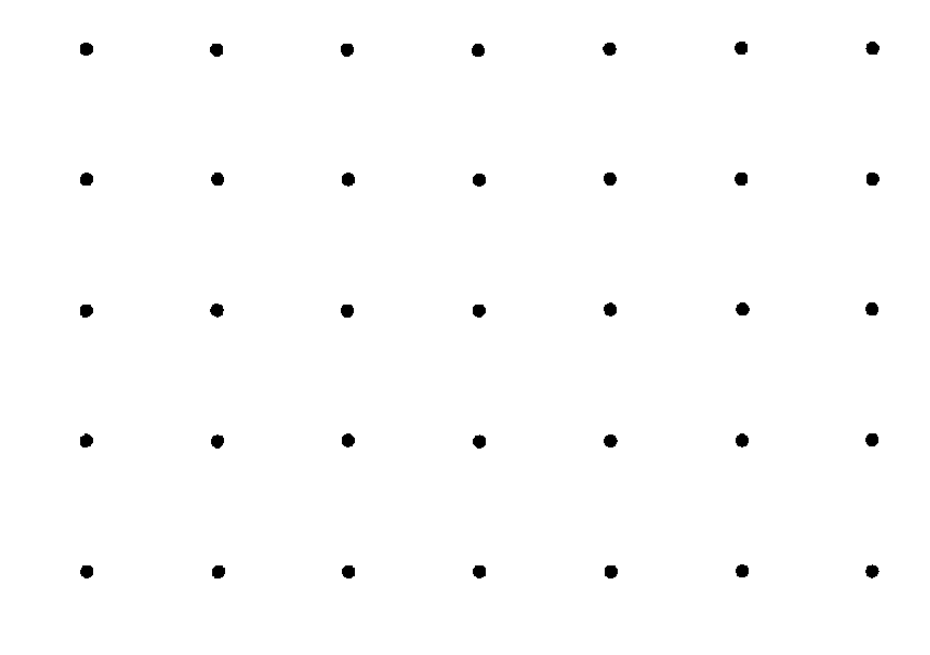
\includegraphics[width=0.60\textwidth]{figures/fig1_6.png}
\caption{The square 2-dimensional Bravais lattice, $p$.}
\end{figure}

corners of squares, is imagined to continue off the diagram to infinity, then these points constitute the simple square 2-dimensional Bravais lattice, \textit{p}. There are five different 2-dimensional Bravais lattices (Alexander 1929, Alexander and Herrmann 1929, Belov 1959\textit{b}) and they are described and illustrated in Volume 1 of the \textit{International tables for X-ray crystallography} (Henry and Lonsdale 1965). In a 3-dimensional Euclidean space, $E(3)$, there are 14 essentially different lattices possible and these are called the (3-dimensional) \textit{Bravais lattices} (Bravais 1849\textit{a}, \textit{b}, 1850). It should perhaps be emphasized that there is not necessarily a Bravais lattice point at the centre of every atom in a real crystal, nor is it necessary for Bravais lattice points to be occupied by atoms.

If we choose one particular lattice point to be the origin, $O$, then we may write $\mathbf{t}$, the position vector of any other lattice point, as

\begin{equation*}
\mathbf{t} = n_{1}\mathbf{t}_{1} + n_{2}\mathbf{t}_{2} + n_{3}\mathbf{t}_{3} \tag{1.5.1}
\end{equation*}

where $n_{1}$, $n_{2}$, and $n_{3}$ are integers and $\mathbf{t}_{1}$, $\mathbf{t}_{2}$, and $\mathbf{t}_{3}$ are the fundamental translations that join $O$ to three of its (non-coplanar) nearest neighbours. The translation operations $\mathbf{t}$ defined by eqn. (1.5.1) form an infinite group which is called the \textit{translation group} of the Bravais lattice. In addition to the symmetry of the group of translations, the Bravais lattice is also invariant under certain point-group operations acting at the lattice points and, sometimes at least, at other points too. The point-group operations at any lattice point form a point group $\mathbf{P}$, which is in fact the holosymmetric point group of one of the crystal systems or syngonies, i.e. $\mathbf{P}$ is the point group with the largest number of symmetry operations in the crystal system in question. In the example of the 2-dimensional Bravais lattice illustrated in Fig. 1.6 the lattice has the symmetry of the point group $4mm$ ($C_{4v}$), or $4/mmm$ ($D_{4h}$) if the dots are on both the back and front of the page. The holosymmetric point groups $\mathbf{P}$, of the seven crystal systems, the triclinic, monoclinic, orthorhombic, tetragonal, trigonal, hexagonal, and cubic are $\bar{1}$ ($C_{i}$), $2/m$ ($C_{2h}$), $mmm$ ($D_{2h}$), $4/mmm$ ($D_{4h}$), $\bar{3}m$ ($D_{3d}$), $6/mmm$ ($D_{6h}$), and $m3m$ ($O_{h}$) respectively. The fact that the point group $\mathbf{P}$ is the holosymmetric point group of the relevant crystal system arises from the following facts: (i) $\mathbf{P}$ must contain the space-inversion operation because if $\mathbf{t}$ is a vector of the Bravais lattice then so also is $-\mathbf{t}$, and (ii) together with axes of orders 3, 4, and 6, $\mathbf{P}$ also contains reflection planes that pass through these axes. It is therefore possible to assign each of the 14 Bravais lattices to one of the seven crystal systems and these Bravais lattices are illustrated in Fig. 1.7. Basically it is because the point-group symmetry of a crystalline solid must be compatible with the symmetry of the Bravais lattice of that solid that there are only 32 possible crystallographic point groups. Each of the 32 crystallographic point groups is either the point group of one of the Bravais lattices, i.e., the holosymmetric point group of one of the seven crystal systems, or else it is a subgroup of one of these seven point groups.

We have said that a Bravais lattice in three dimensions is an infinite array of points

\begin{figure}[H]
\centering
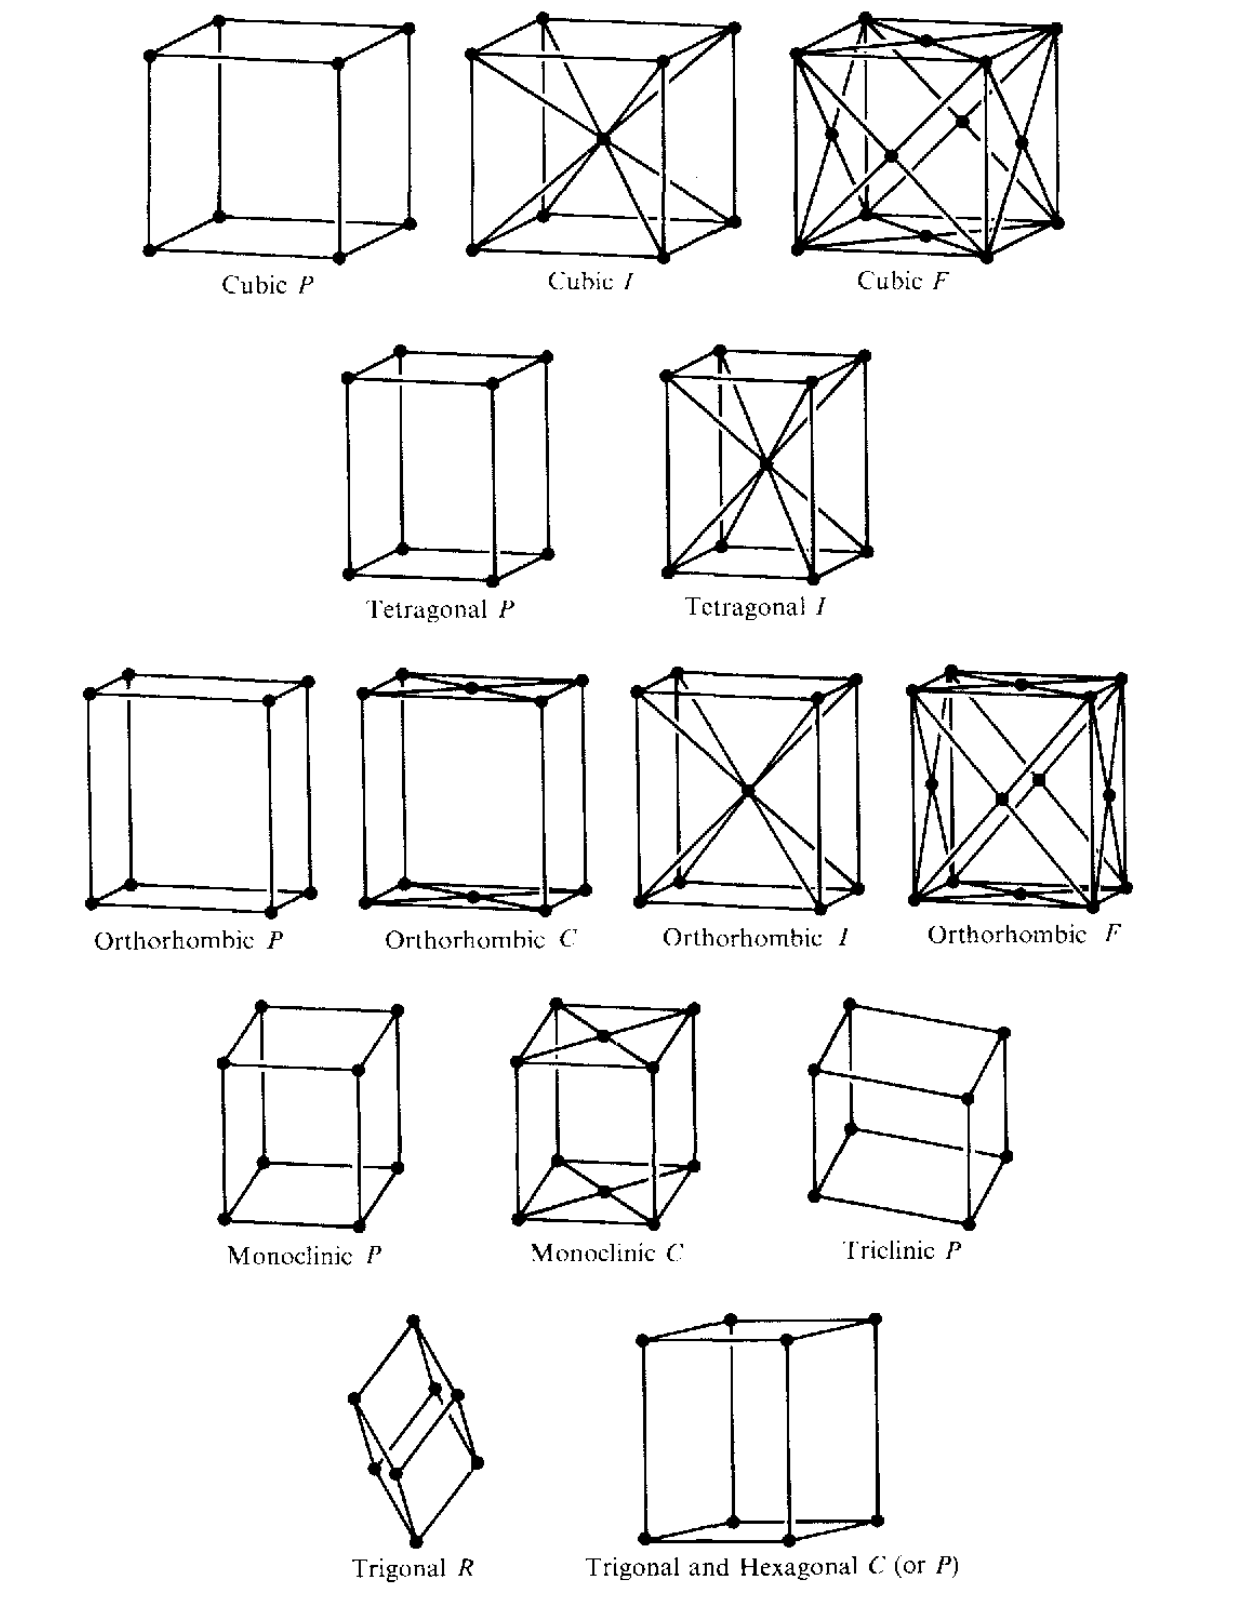
\includegraphics[width=0.98\textwidth]{figures/fig1_7.png}
\caption{The 14 Bravais lattices (Phillips 1963\textit{a}).}
\end{figure}

\begin{figure}[H]
\centering
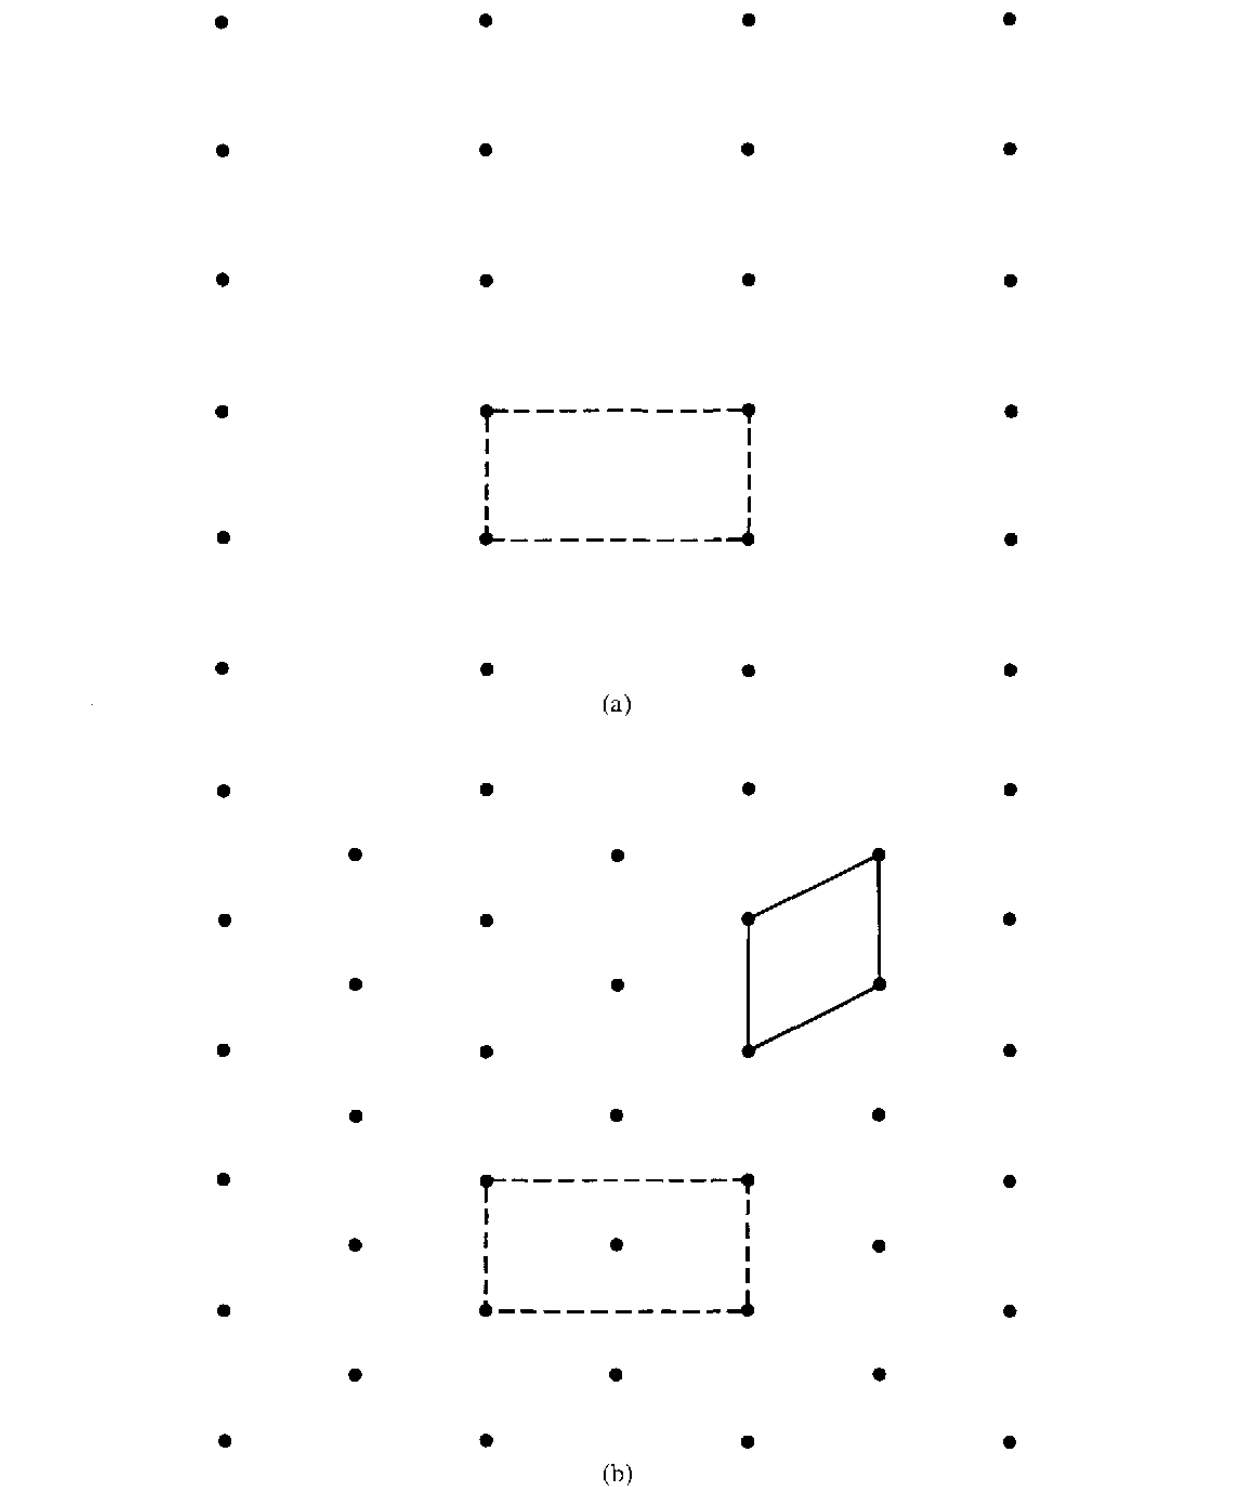
\includegraphics[width=0.98\textwidth]{figures/fig1_8.png}
\caption{(a) The rectangular 2-dimensional Bravais lattice, \textit{p}, with unit cell marked. (b) The centred rectangular 2-dimensional Bravais lattice, \textit{c}, with conventional unit cell shown with broken lines and fundamental unit cell shown with continuous lines.}
\end{figure}

such that each point has the same environment in the same orientation. A \textit{unit cell} may be defined in various ways and it will be specified by three non-coplanar vectors which form the edges of a parallelepiped. The symbols $\mathbf{a}$, $\mathbf{b}$, and $\mathbf{c}$ are used to denote these three vectors. It is usually convenient to select the unit-cell vectors in such a way that the unit cell clearly exhibits the symmetry of the lattice. This conventional choice of unit cell may then not be primitive, that is, it may contain the equivalent of more than one lattice point. The parallelepiped constructed on the three basic vectors $\mathbf{t}_{1}$, $\mathbf{t}_{2}$, and $\mathbf{t}_{3}$ of the Bravais lattice (eqn. (1.5.1)) is called the \textit{primitive unit cell}. In each Bravais lattice where the conventional unit cell and the primitive unit cell are not identical it is possible to establish the relationship between them. This is done for instance in Table 2.2.2 of Volume 1 of the \textit{International tables for X-ray crystallography}. The unit cells illustrated in Fig. 1.7 are the conventional unit cells. The actual specification of $\mathbf{t}_{1}$, $\mathbf{t}_{2}$, and $\mathbf{t}_{3}$ for each of the 14 Bravais lattices will be given in Chapter 3 (Table 3.1). We can illustrate the distinction between conventional and primitive unit cells with a 2-dimensional example. The 2-dimensional primitive rectangular Bravais lattice, \textit{p}, has its lattice points arranged on the corners of a set of rectangles and the conventional unit cell is one such rectangle, see Fig. 1.8(\textit{a}); this is also a fundamental unit cell of this lattice. If a point is added to the centre of each of these cells a new Bravais lattice is obtained, the centred rectangular Bravais lattice, \textit{c}, see Fig. 1.8(\textit{b}). A conventional unit cell, which exhibits the rectangular symmetry, is shown with broken lines and a primitive unit cell is shown with continuous lines. The conventional unit cell contains effectively two lattice points while the primitive unit cell contains only one lattice point. Another unit cell that is sometimes used is the \textit{Wigner–Seitz unit cell} (Wigner and Seitz 1933). The Wigner–Seitz unit cell of a Bravais lattice is obtained by choosing as origin, $O$, any one of the lattice points and drawing the planes that bisect perpendicularly the lines joining $O$ to its nearest (and sometimes to its next-nearest) neighbours. The unit cell bounded by these planes is called the Wigner–Seitz unit cell; these unit cells are illustrated, for example, by Delaunay (1932).

A Bravais lattice, as we have described it, is an array of mathematical points that have position but no magnitude or shape. We now wish to include in our discussion the atoms or molecules of which the crystal is constituted. We are then effectively associating a similar collection of atoms with each Bravais lattice point and this set of atoms or molecules must itself possess symmetry that is compatible with the point-group symmetry of the Bravais lattice of the crystal. One type of symmetry operation of the crystal will be a compound operation consisting of some point-group operation followed by a translation $\mathbf{t}$ (see eqn. (1.5.1)) of the Bravais lattice. Thus, an especially simple type of \textit{space group} arises by associating with each point of a Bravais lattice one of the point groups belonging to the same crystal system. In this way it is possible to obtain $\sum_{i=1}^{7} n_{i}p_{i}$ space groups where $n_{i}$ is the number of point groups in a certain crystal system and $p_{i}$ is the number of Bravais lattices in that system, the suffix \textit{i} ranging over the seven crystal systems. For example, there are three cubic Bravais lattices and five cubic point groups, so that there are 15 cubic space groups that can be derived in this way. A space group of this form is said to be \textit{symmorphic} and it is a semi-direct product group of the translation group of the Bravais lattice and a point group. The theory of semi-direct product groups will be discussed in Chapter 4. The above formula does not at once account for all the symmorphic space groups; there are two reasons for this. First, it is possible to associate a trigonal point group with the hexagonal Bravais lattice: so for the trigonal system we must take $p_{i} = 2$ even though there is only one trigonal Bravais lattice. Secondly, it does in fact happen that there can sometimes be two different and distinguishable orientations of a point group possible on a Bravais lattice; this leads to a few extra symmorphic space groups that occur irregularly as shown in column 6 of Table 1.7. There are in fact 73 different symmorphic space groups.

In a symmorphic space group the point-group operations and the operations of the translation group are essentially separable and the point-group operations that are present are, on their own, symmetry operations of the crystal. A second type of space group can arise by starting with a symmorphic space group and replacing some of the reflection planes by glide reflection planes and some of the rotation axes by screw rotation axes; these are commonly called glide planes and screw axes respectively. A glide reflection symmetry operation is a compound operation that consists of a reflection in a plane, \textit{m}, together with a translation $\mathbf{v}$, which is often, but not necessarily, in the plane \textit{m} itself. The final result of two successive performances of such a glide reflection operation is to produce a translation that must itself be a member of the group of translations of the Bravais lattice of the crystal. In a similar way we may have a screw axis of order \textit{n}: a screw rotation symmetry operation consists of a rotation through $2\pi/n$ about an axis, followed by a translation, $\mathbf{v}$, which is often, but not necessarily, along the axis of rotation. If this screw rotation operation is performed $n$ times in succession, the result is a pure translation that must again be a member of the group of translations of the Bravais lattice of the crystal. By including glide reflection planes and screw rotation axes it is possible to derive a further 157 space groups that are called \textit{non-symmorphic space groups} or \textit{asymmorphic space groups}. One can impose the condition that the translational part of each glide reflection operation must be in the reflection plane itself and that the translational part of each screw rotation operation should be along the axis of the rotation. If this condition is imposed then, when there are glide reflection planes or screw rotation axes present, the symmetry elements may not act all at one point in the crystal. When this is so the operators can always be transformed to act at one point but then the translations may lose their sense of being along the axis of the screw rotation or of being in the plane of the glide reflection and may be in some strange direction. The former viewpoint is visually more satisfying, but the latter viewpoint is essential for a systematic mathematical treatment, and we shall therefore adopt the convention that all space-group operations act at one point. The 157 non-symmorphic space groups together with the 73 symmorphic space groups make a total of 230 space groups in all. They are distributed among the crystal systems as shown in Table 1.7.

\begin{minipage}{\textwidth}
\centering\textbf{TABLE 1.7}
\textit{The classification of the 230 space groups}

\noindent\resizebox{\textwidth}{!}{
\centering
\begin{tabular}{|l|l|l|l|l|l|l|l|l|}
\hline
Crystal system & $s$ & $n_{i}$ & $p_{i}$ & $n_{i}p_{i}$ & col. 6 & col. 7 & col. 8 & col. 9 \\ \hline
Triclinic & 1 & 2 & 1 & 2 &  & 2 &  & 2 \\ \hline
Monoclinic & 2 & 3 & 2 & 6 &  & 6 & 7 & 13 \\ \hline
Orthorhombic & -- & 3 & 4 & 12 & 1 & 13 & 46 & 59 \\ \hline
Tetragonal & 4 & 7 & 2 & 14 & 2 & 16 & 52 & 68 \\ \hline
Trigonal & 3 & 5 & 2 & 10 & 3 & 13 & 12 & 25 \\ \hline
Hexagonal & 6 & 7 & 1 & 7 & 1 & 8 & 19 & 27 \\ \hline
Cubic &  & 5 & 3 & 15 &  & 15 & 21 & 36 \\ \hline
\textbf{Total} & -- & 32 & 15 & 66 & 7 & 73 & 157 & 230 \\ \hline
\end{tabular}
}
\end{minipage}
\medskip

\textit{Notes to Table 1.7}

\begin{quote}(i) $s$ is the order of the principal axis in those cases where it exists. The operations about the principal axis can be proper or improper rotations. (ii) $n_{i}$ is the number of point groups of a given system. Note that $\bar{6}$ ($C_{3h}$) and $\bar{6}2m$ ($D_{3h}$) must be allocated to the hexagonal system. $p_{i}$ is the number of Bravais lattices of a given system, except for the trigonal system where $p_{i} = 2$; for as explained in the text each trigonal point group can be associated with the hexagonal Bravais lattice. This lattice is therefore counted twice in the total. (iii) Column 6 is the number of symmorphic space groups that occur because of alternative distinguishable settings of certain point groups on their Bravais lattices. Columns 7 and 8 are the total numbers of symmorphic and non-symmorphic space groups in a given system. Column 9 is the total number of space groups of either kind in a given system.\end{quote}

\textit{Seitz notation for space-group operators}

A convenient notation to represent a general space-group operation is to use the symbol $\{R \,|\, \mathbf{v}\}$ with the meaning that $R$ is a point-group operator and $\mathbf{v}$ is the translation vector to be associated with it; the interpretation of this operator is that it acts on the points of space and that these are always referred to a fixed set of axes, that is, it is an \textit{active} operator (see section 1.4). The symbols $\{R \,|\, \mathbf{v}\}$ were introduced by Seitz (1936\textit{b}) and they are called \textit{Seitz space-group symbols}. Since these operators are active, $\{R_{1} \,|\, \mathbf{v}_{1}\}$ operating on the vector $\mathbf{r}$ produces $\mathbf{r}'$, so that

\begin{equation*}
\{R_{1} \,|\, \mathbf{v}_{1}\}\mathbf{r} = \mathbf{r}' = R_{1}\mathbf{r} + \mathbf{v}_{1}, \tag{1.5.2}
\end{equation*}

where $R_{1}\mathbf{r}$ is the vector that is produced from $\mathbf{r}$ by the application of the active point-group operator $R_{1}$. There is a simple but important rule for the multiplication of these operators:

\begin{equation*}
\{R_{2} \,|\, \mathbf{v}_{2}\}\{R_{1} \,|\, \mathbf{v}_{1}\} = \{R_{2}R_{1} \,|\, \mathbf{v}_{2} + R_{2}\mathbf{v}_{1}\} \tag{1.5.3}
\end{equation*}
 as can easily be verified by applying $\{R_{2} \,|\, \mathbf{v}_{2}\}$ to both sides of eqn. (1.5.2). From eqn. (1.5.3) it follows immediately that the inverse of $\{R_{1} \,|\, \mathbf{v}_{1}\}$ is $\{R_{1}^{-1} | -R_{1}^{-1}\mathbf{v}_{1}\}$. The Seitz operators for all the 230 space groups are identified by various authors (Faddeev 1964, Henry and Lonsdale 1965, Koptsik 1966, Kovalev 1965, Lyubarskii 1960, Miller and Love 1967) and they are listed in Chapter 3.

\textit{Notation for the labels of the space groups}

A space group is classified first by the crystal system to which it belongs. Any secondary classification depends upon how much information one wants to convey. It is possible to label the point group to which the space group is \textit{isogonal}, that is, the point group which is obtained by taking all the point-group operators present from amongst the operations of the space-group.\textsuperscript{\ddag} This is the position that is adopted when using the Schönflies notation (Hilton 1903). In this notation the space group is given the Schönflies label of its isogonal point group and different space groups having the same isogonal point group are given an arbitrary distinguishing superscript. This represented merely the order in which Schönflies (1891) presented the derivation of the space groups. There are, for example, 10 space groups isogonal to the cubic point group $O_{h}$ ($m3m$) and these are distributed among the three cubic Bravais lattices, four primitive, four face-centred and two body-centred, and they are numbered $O_{h}^{1}$, $O_{h}^{2}$, ..., $O_{h}^{10}$. This notation has two disadvantages. First, it is not possible to tell at a glance on which Bravais lattice the space group is based: for example, $O_{h}^{8}$ is face-centred and $O_{h}^{6}$ is body-centred. Secondly, there is no indication of whether the space group is symmorphic or non-symmorphic. An even more arbitrary scheme in which each space group is given a number between 1 and 230 was developed by Astbury and Yardley (1924) and has been included in the \textit{International tables for X-ray crystallography} (Henry and Lonsdale 1965).

The two disadvantages of the Schönflies notation are overcome by using the international notation, which not only determines the two features just mentioned but also gives some idea of the nature and orientation of the symmetry elements present in the space group (Hermann 1928\textit{a}, Mauguin 1931, Schiebold 1929). Starting with the international point-group symbol, for example $m3m$, this is prefixed by the letter describing the Bravais lattice, for example \textit{P}, \textit{F}, \textit{I}, for primitive, face-centred, and body-centred respectively, so that we obtain the symbols $Pm3m$, $Fm3m$, and $Im3m$. These symbols denote the three symmorphic space groups isogonal to the point group $m3m$ ($O_{h}$). When a point group can be situated on a Bravais lattice in more than one orientation, as for instance $\bar{4}2m$ ($D_{2d}$) in the tetragonal system, this is allowed for by attaching significance to the ordering of the characters in the international space-group symbol; thus $P\bar{4}2m$ ($D_{2d}$) and $P\bar{4}m2$ ($D_{2d}$) are distinct space groups. For non-symmorphic space groups the symbol is modified as follows. For any reflection plane

that has been replaced by a glide plane the appropriate part of the symbol is replaced by another letter denoting a glide plane; thus $Fd3m$ ($O_{h}^{7}$), the space group of the diamond structure, is face-centred and non-symmorphic, with glide planes in a diagonal direction. Other letters used include the crystal axis directions \textit{a}, \textit{b}, and \textit{c}. For a screw axis the part of the space-group symbol denoting the order of such an axis, for example 4 of $P432$, is replaced by the same symbol with an added suffix denoting the size of the translation of the screw axis. Thus $P4_{1}32$ ($O^{7}$), one of the cubic space groups isogonal to the point group 432 ($O$), is primitive with the fourfold rotation axis replaced by a fourfold screw axis so that a translation of one-quarter of a lattice vector in that direction is associated with each of the fourfold rotations. The international notation is not perfect, but is well known, carefully identified (Henry and Lonsdale 1965), and widely accepted. The original form of this notation is explained in the old \textit{International tables for X-ray crystallography} (Bragg, von Laue, and Hermann 1935\textit{a}, \textit{b}) and the later modifications are explained in the new tables (Henry and Lonsdale 1965); the use of these tables in the identification of space groups will be discussed further in Chapter 3 (see section 3.5). In this book we always refer to a point group or space group by its international symbol followed by its Schönflies symbol in brackets.

\textit{Function space operators}

If $R$ is the rotational part of a Seitz space-group operator, that is, $R$ is a point-group operation, then each operator $R$ acts on the points of space $\mathbf{r}$ by means of an equation like eqn. (1.4.8),

\begin{equation*}
R\mathbf{r} = \mathbf{r}'. \tag{1.5.4}
\end{equation*}

If a scalar function $f(\mathbf{r})$ is defined then the movement of the points $\mathbf{r}$ will induce a corresponding change in the function. This new function will be such that the new function at the transformed point is equal in value to the old function at the original point. That is to say,

\begin{equation*}
g(\mathbf{r}') = f(\mathbf{r}). \tag{1.5.5}
\end{equation*}

It is customary to write $g = \bar{R}f$, so that to each operator $R$ there is defined a corresponding \textit{function space operator} $\bar{R}$. From eqns. (1.5.4) and (1.5.5) it follows that

\begin{equation*}
\bar{R}f(\mathbf{r}) = f(R^{-1}\mathbf{r}). \tag{1.5.6}
\end{equation*}

It is perhaps unfortunate, but nevertheless a fact, that most writers do not use a separate symbol for $\bar{R}$ and indeed there is no need for a separate symbol provided one distinguishes carefully whether the operator is acting on a function or on a vector. Care must be taken to manipulate function space operators by means of eqn. (1.5.6). The following examples should act as sufficient warning.

\textit{Example} 1.5.1. Let $\mathbf{r} = x\mathbf{i} + y\mathbf{j} + z\mathbf{k}$, and define $f(\mathbf{r}) = x$, $g(\mathbf{r}) = y$, and $h(\mathbf{r}) = z$, the projections of the vector $\mathbf{r}$ in the three coordinate directions. Then

\begin{equation*}
\bar{C}_{4z}^{+}f(\mathbf{r}) = f(C_{4z}^{+}\mathbf{r}), \tag{1.5.7}
\end{equation*}

which is equal to $f(y\mathbf{i} - x\mathbf{j} + z\mathbf{k})$ (see Note (iii) to Table 1.4). The projection of the argument in the direction $\mathbf{i}$ is $y$ so that

\begin{equation*}
\bar{C}_{4z}^{+}f(\mathbf{r}) = y = g(\mathbf{r}). \tag{1.5.8}
\end{equation*}

Symbolically we have therefore both $C_{4z}^{+}\mathbf{i} = \mathbf{j}$ and $\bar{C}_{4z}^{+}f = g$. Indeed the matrix representing the operator $C_{4z}^{+}$ with respect to the basis $\langle \mathbf{i}, \mathbf{j}, \mathbf{k}|$ is the same as the matrix representing the function space operator $\bar{C}_{4z}^{+}$ with respect to the basis $\langle f, g, h|$. After the warning to be careful this is a result that one would scarcely have dared to expect to be true.

\textit{Example} 1.5.2. Let $\phi$ be the azimuthal angle (the angle between the $x$-axis and the projection of the position vector onto the $xy$-plane). Then

\begin{equation*}
C_{4z}^{+}\phi = \phi + \tfrac{1}{2}\pi \tag{1.5.9}
\end{equation*}

but for $\bar{C}_{4z}^{+}$ as a function space operator we must write

\begin{equation*}
\bar{C}_{4z}^{+}\cos\phi = \cos(C_{4z}^{-}\phi) = \cos(\phi - \tfrac{1}{2}\pi) = \sin\phi. \tag{1.5.10}
\end{equation*}

Equation (1.5.10) could have been deduced also from eqn. (1.5.8), because $f(\mathbf{r}) = r\sin\theta\cos\phi$ and $g(\mathbf{r}) = r\sin\theta\sin\phi$, and $C_{4z}^{+}$ leaves $r$ and $\theta$ unaltered. It should be noted that, since $\cos(\phi + \tfrac{1}{2}\pi) = -\sin\phi$, $C_{4z}^{+}\cos\phi \neq \cos(C_{4z}^{+}\phi)$.

\textit{Active and passive space-group operators}

As we have already pointed out an active operator is one that moves the points or position vectors of space, all vectors being referred to a fixed set of axes. The Seitz space-group operators that we shall use in this book are active and have been defined by eqn. (1.5.2). The definition is

\begin{equation*}
\{R_{a} \,|\, \mathbf{v}\}\mathbf{r} = R_{a}\mathbf{r} + \mathbf{v}, \tag{1.5.11}
\end{equation*}

where we use the subscript $a$ to emphasize that we mean an active operator. That is to say, an active rotation $R_{a}$ is made first so that $\mathbf{r} \rightarrow R_{a}\mathbf{r}$ and then a translation $+\mathbf{v}$ is made to the new position vector, the result being $(R_{a}\mathbf{r} + \mathbf{v})$. We have already found the multiplication rule for the active Seitz space-group operators in eqn. (1.5.3), namely

\begin{equation*}
\{S_{a} \,|\, \mathbf{w}\}\{R_{a} \,|\, \mathbf{v}\} = \{S_{a}R_{a} \,|\, \mathbf{w} + S_{a}\mathbf{v}\}. \tag{1.5.12}
\end{equation*}

The inverse of $\{R_{a} \,|\, \mathbf{v}\}$ is

\begin{equation*}
\{R_{a} \,|\, \mathbf{v}\}^{-1} = \{R_{a}^{-1} \,|\, -R_{a}^{-1}\mathbf{v}\}. \tag{1.5.13}
\end{equation*}

A passive operator is one that moves the axes of space, all points of the space and hence all vector positions being left unmoved, so that after each operation a vector position is referred to a new set of axes. It is possible to define passive space-group operators (Johnston 1960). To distinguish them from active Seitz operators we use square brackets $[R_{p} \,|\, \mathbf{v}]$ and the rule of definition corresponding to eqn. (1.5.11) is

\begin{equation*}
[R_{p} \,|\, \mathbf{v}]\mathbf{r} = R_{p}\mathbf{r} - R_{p}\mathbf{v}. \tag{1.5.14}
\end{equation*}

That is to say a translation of axes by $+\mathbf{v}$ is made first so that $\mathbf{r} \rightarrow (\mathbf{r} - \mathbf{v})$, and then a rotation of the new axes is made, the final result being $(R_{p}\mathbf{r} - R_{p}\mathbf{v})$, where $R_{p}$ is now a passive rotation. The rule for the multiplication of these passive operators is

\begin{equation*}
[S_{p} \,|\, \mathbf{w}][R_{p} \,|\, \mathbf{v}] = [S_{p}R_{p} \,|\, \mathbf{v} + R_{p}^{-1}\mathbf{w}] \tag{1.5.15}
\end{equation*}

and the inverse of $[R_{p} \,|\, \mathbf{v}]$ is

\begin{equation*}
[R_{p} \,|\, \mathbf{v}]^{-1} = [R_{p}^{-1} \,|\, -R_{p}\mathbf{v}]. \tag{1.5.16}
\end{equation*}

If $X$ is an operator, whether active or passive, then along with $X$ there is another operator $\bar{X}$ where $\bar{X}$ is a function-space operator as defined in eqns. (1.5.4)–(1.5.6). If $f(\mathbf{r})$ is a scalar function of position then

\begin{equation*}
\bar{X}f(\mathbf{r}) = f(X^{-1}\mathbf{r}). \tag{1.5.17}
\end{equation*}

It is important to realize that $(\bar{X}f)$ is the symbol for a function just as $f$ is also the symbol for a function. Equation (1.5.17) is not arbitrary but states the fact that the value of the transformed function $(\bar{X}f)$ at the transformed point $X\mathbf{r}$ is equal in value to $f$ at the point $\mathbf{r}$. Another point, stressed by Wigner (1959), must again be emphasized, and that is that if $Z = YX$ then we require $\bar{Z}f = \bar{Y}\bar{X}f$ because we want to preserve an isomorphism between groups of operators and the corresponding groups of function-space operators. The proof that this is true follows from repeated application of eqn. (1.5.17). If we write $\bar{X}f = g$ then

\begin{align*}
\bar{Y}\bar{X}f(\mathbf{r}) &= \bar{Y}g(\mathbf{r}), \\
&= g(Y^{-1}\mathbf{r}) &&\text{(from eqn. (1.5.17))}, \\
&= \bar{X}f(Y^{-1}\mathbf{r}) &&\text{(since $\bar{X}f = g$)}, \\
&= f(X^{-1}Y^{-1}\mathbf{r}) &&\text{(from eqn. (1.5.17))}, \\
&= f(Z^{-1}\mathbf{r}) &&\text{(since $Z = YX$)}, \\
&= \bar{Z}f(\mathbf{r}) &&\text{(from eqn. (1.5.17) again)}.
\end{align*}

Thus $\bar{Y}\bar{X}f = \bar{Z}f$ as required. It is incorrect to operate directly on eqn. (1.5.17) with $\bar{Y}$ since it is a numerical relationship between two functions for different values of their arguments and operators cannot act on numbers (Altmann and Bradley 1965, Slater 1965\textit{a}).

As a first example let us consider the effect of passive space-group operators on a function $\psi(\mathbf{r})$. From eqn. (1.5.17) it follows that

\begin{align*}
\overline{[S_{p} \,|\, \mathbf{w}]}\,\psi(\mathbf{r}) &= \psi([S_{p} \,|\, \mathbf{w}]^{-1}\mathbf{r}) \\
&= \psi([S_{p}^{-1} \,|\, -S_{p}\mathbf{w}]\mathbf{r}) &&\text{(from eqn. (1.5.16))} \tag{1.5.18}\\
&= \psi(S_{p}^{-1}\mathbf{r} + \mathbf{w}) &&\text{(from eqn. (1.5.14))}. \tag{1.5.19}
\end{align*}

From the rule for multiplying function-space operators and from eqn. (1.5.19)

\begin{align*}
\overline{[S_{p} \,|\, \mathbf{w}]}\,\overline{[R_{p} \,|\, \mathbf{v}]}\,\psi(\mathbf{r}) &= \overline{[R_{p} \,|\, \mathbf{v}]}\,\psi(S_{p}^{-1}\mathbf{r} + \mathbf{w}) \\
&= \psi(R_{p}^{-1}S_{p}^{-1}\mathbf{r} + R_{p}^{-1}\mathbf{w} + \mathbf{v}). \tag{1.5.20}
\end{align*}

A derivation of eqn. (1.5.20) from eqn. (1.5.19) as follows would not be correct:

\begin{align*}
\overline{[S_{p} \,|\, \mathbf{w}]}\,\overline{[R_{p} \,|\, \mathbf{v}]}\,\psi(\mathbf{r}) &= \overline{[S_{p} \,|\, \mathbf{w}]}\,\psi(R_{p}^{-1}\mathbf{r} + \mathbf{v}) \tag{1.5.21}\\
&= \psi(R_{p}^{-1}(S_{p}^{-1}\mathbf{r} + \mathbf{w}) + \mathbf{v}) \tag{1.5.22}\\
&= \psi(R_{p}^{-1}S_{p}^{-1}\mathbf{r} + R_{p}^{-1}\mathbf{w} + \mathbf{v}). \tag{1.5.20}
\end{align*}

Equation (1.5.21) is incorrect because, as mentioned above, $[S_{p} \,|\, \mathbf{w}]$ cannot be applied directly to the numerical relationship $[R_{p} \,|\, \mathbf{v}]\psi(\mathbf{r}) = \psi(R_{p}^{-1}\mathbf{r} + \mathbf{v})$; but just supposing it could, then eqn. (1.5.22) is also at fault, and is directly contrary to mathematical practice, because a function-space operator acts on the whole of the argument of a function and not just the part $\mathbf{r}$.

The equations corresponding to (1.5.19) and (1.5.20) for active space-group operators are

\begin{equation*}
\overline{\{S_{a} \,|\, \mathbf{w}\}}\,\psi(\mathbf{r}) = \psi(S_{a}^{-1}(\mathbf{r} - \mathbf{w})) \tag{1.5.23}
\end{equation*}

and

\begin{equation*}
\overline{\{S_{a} \,|\, \mathbf{w}\}}\,\overline{\{R_{a} \,|\, \mathbf{v}\}}\,\psi(\mathbf{r}) = \psi(R_{a}^{-1}S_{a}^{-1}\mathbf{r} - R_{a}^{-1}S_{a}^{-1}\mathbf{w} - R_{a}^{-1}\mathbf{v}). \tag{1.5.24}
\end{equation*}

Equations (1.5.19) and (1.5.23) plus the fact that $S_{p} = S_{a}^{-1}$ imply that $[S_{p} \,|\, \mathbf{w}] = \{S_{a} \,|\, \mathbf{w}\}^{-1}$ a relationship that we should expect to hold between active and passive operators.

\textit{Example} 1.5.3. Let $\{E \,|\, \mathbf{t}\}$ denote the translation $\mathbf{t}$. Then

\begin{equation*}
\{E \,|\, \mathbf{t}\}\mathbf{r} = \mathbf{r} + \mathbf{t}. \tag{1.5.25}
\end{equation*}

But if $\{E \,|\, \mathbf{t}\}$ now acts on the function $\psi(\mathbf{r})$ rather than on the vector $\mathbf{r}$ we have

\begin{equation*}
\overline{\{E \,|\, \mathbf{t}\}}\,\psi(\mathbf{r}) = \psi(\{E \,|\, \mathbf{t}\}^{-1}\mathbf{r}) = \psi(\mathbf{r} - \mathbf{t}). \tag{1.5.26}
\end{equation*}

As we have said before, we shall always use active point-group and space-group operators in this book, except that we shall occasionally illustrate how our theoretical discussions would have to be modified if one did choose to use passive operators.

\end{document}
